% Options for packages loaded elsewhere
\PassOptionsToPackage{unicode}{hyperref}
\PassOptionsToPackage{hyphens}{url}
\PassOptionsToPackage{dvipsnames,svgnames,x11names}{xcolor}
%
\documentclass[
  a4paper,
  DIV=11,
  numbers=noendperiod,
  oneside]{scrreprt}

\usepackage{amsmath,amssymb}
\usepackage{iftex}
\ifPDFTeX
  \usepackage[T1]{fontenc}
  \usepackage[utf8]{inputenc}
  \usepackage{textcomp} % provide euro and other symbols
\else % if luatex or xetex
  \usepackage{unicode-math}
  \defaultfontfeatures{Scale=MatchLowercase}
  \defaultfontfeatures[\rmfamily]{Ligatures=TeX,Scale=1}
\fi
\usepackage{lmodern}
\ifPDFTeX\else  
    % xetex/luatex font selection
\fi
% Use upquote if available, for straight quotes in verbatim environments
\IfFileExists{upquote.sty}{\usepackage{upquote}}{}
\IfFileExists{microtype.sty}{% use microtype if available
  \usepackage[]{microtype}
  \UseMicrotypeSet[protrusion]{basicmath} % disable protrusion for tt fonts
}{}
\makeatletter
\@ifundefined{KOMAClassName}{% if non-KOMA class
  \IfFileExists{parskip.sty}{%
    \usepackage{parskip}
  }{% else
    \setlength{\parindent}{0pt}
    \setlength{\parskip}{6pt plus 2pt minus 1pt}}
}{% if KOMA class
  \KOMAoptions{parskip=half}}
\makeatother
\usepackage{xcolor}
\ifLuaTeX
  \usepackage{luacolor}
  \usepackage[soul]{lua-ul}
\else
  \usepackage{soul}
  
\fi
\setlength{\emergencystretch}{3em} % prevent overfull lines
\setcounter{secnumdepth}{5}
% Make \paragraph and \subparagraph free-standing
\makeatletter
\ifx\paragraph\undefined\else
  \let\oldparagraph\paragraph
  \renewcommand{\paragraph}{
    \@ifstar
      \xxxParagraphStar
      \xxxParagraphNoStar
  }
  \newcommand{\xxxParagraphStar}[1]{\oldparagraph*{#1}\mbox{}}
  \newcommand{\xxxParagraphNoStar}[1]{\oldparagraph{#1}\mbox{}}
\fi
\ifx\subparagraph\undefined\else
  \let\oldsubparagraph\subparagraph
  \renewcommand{\subparagraph}{
    \@ifstar
      \xxxSubParagraphStar
      \xxxSubParagraphNoStar
  }
  \newcommand{\xxxSubParagraphStar}[1]{\oldsubparagraph*{#1}\mbox{}}
  \newcommand{\xxxSubParagraphNoStar}[1]{\oldsubparagraph{#1}\mbox{}}
\fi
\makeatother


\providecommand{\tightlist}{%
  \setlength{\itemsep}{0pt}\setlength{\parskip}{0pt}}\usepackage{longtable,booktabs,array}
\usepackage{multirow}
\usepackage{calc} % for calculating minipage widths
% Correct order of tables after \paragraph or \subparagraph
\usepackage{etoolbox}
\makeatletter
\patchcmd\longtable{\par}{\if@noskipsec\mbox{}\fi\par}{}{}
\makeatother
% Allow footnotes in longtable head/foot
\IfFileExists{footnotehyper.sty}{\usepackage{footnotehyper}}{\usepackage{footnote}}
\makesavenoteenv{longtable}
\usepackage{graphicx}
\makeatletter
\def\maxwidth{\ifdim\Gin@nat@width>\linewidth\linewidth\else\Gin@nat@width\fi}
\def\maxheight{\ifdim\Gin@nat@height>\textheight\textheight\else\Gin@nat@height\fi}
\makeatother
% Scale images if necessary, so that they will not overflow the page
% margins by default, and it is still possible to overwrite the defaults
% using explicit options in \includegraphics[width, height, ...]{}
\setkeys{Gin}{width=\maxwidth,height=\maxheight,keepaspectratio}
% Set default figure placement to htbp
\makeatletter
\def\fps@figure{htbp}
\makeatother

\usepackage{my-conf-quarto}
\subtitle{\vspace{3cm}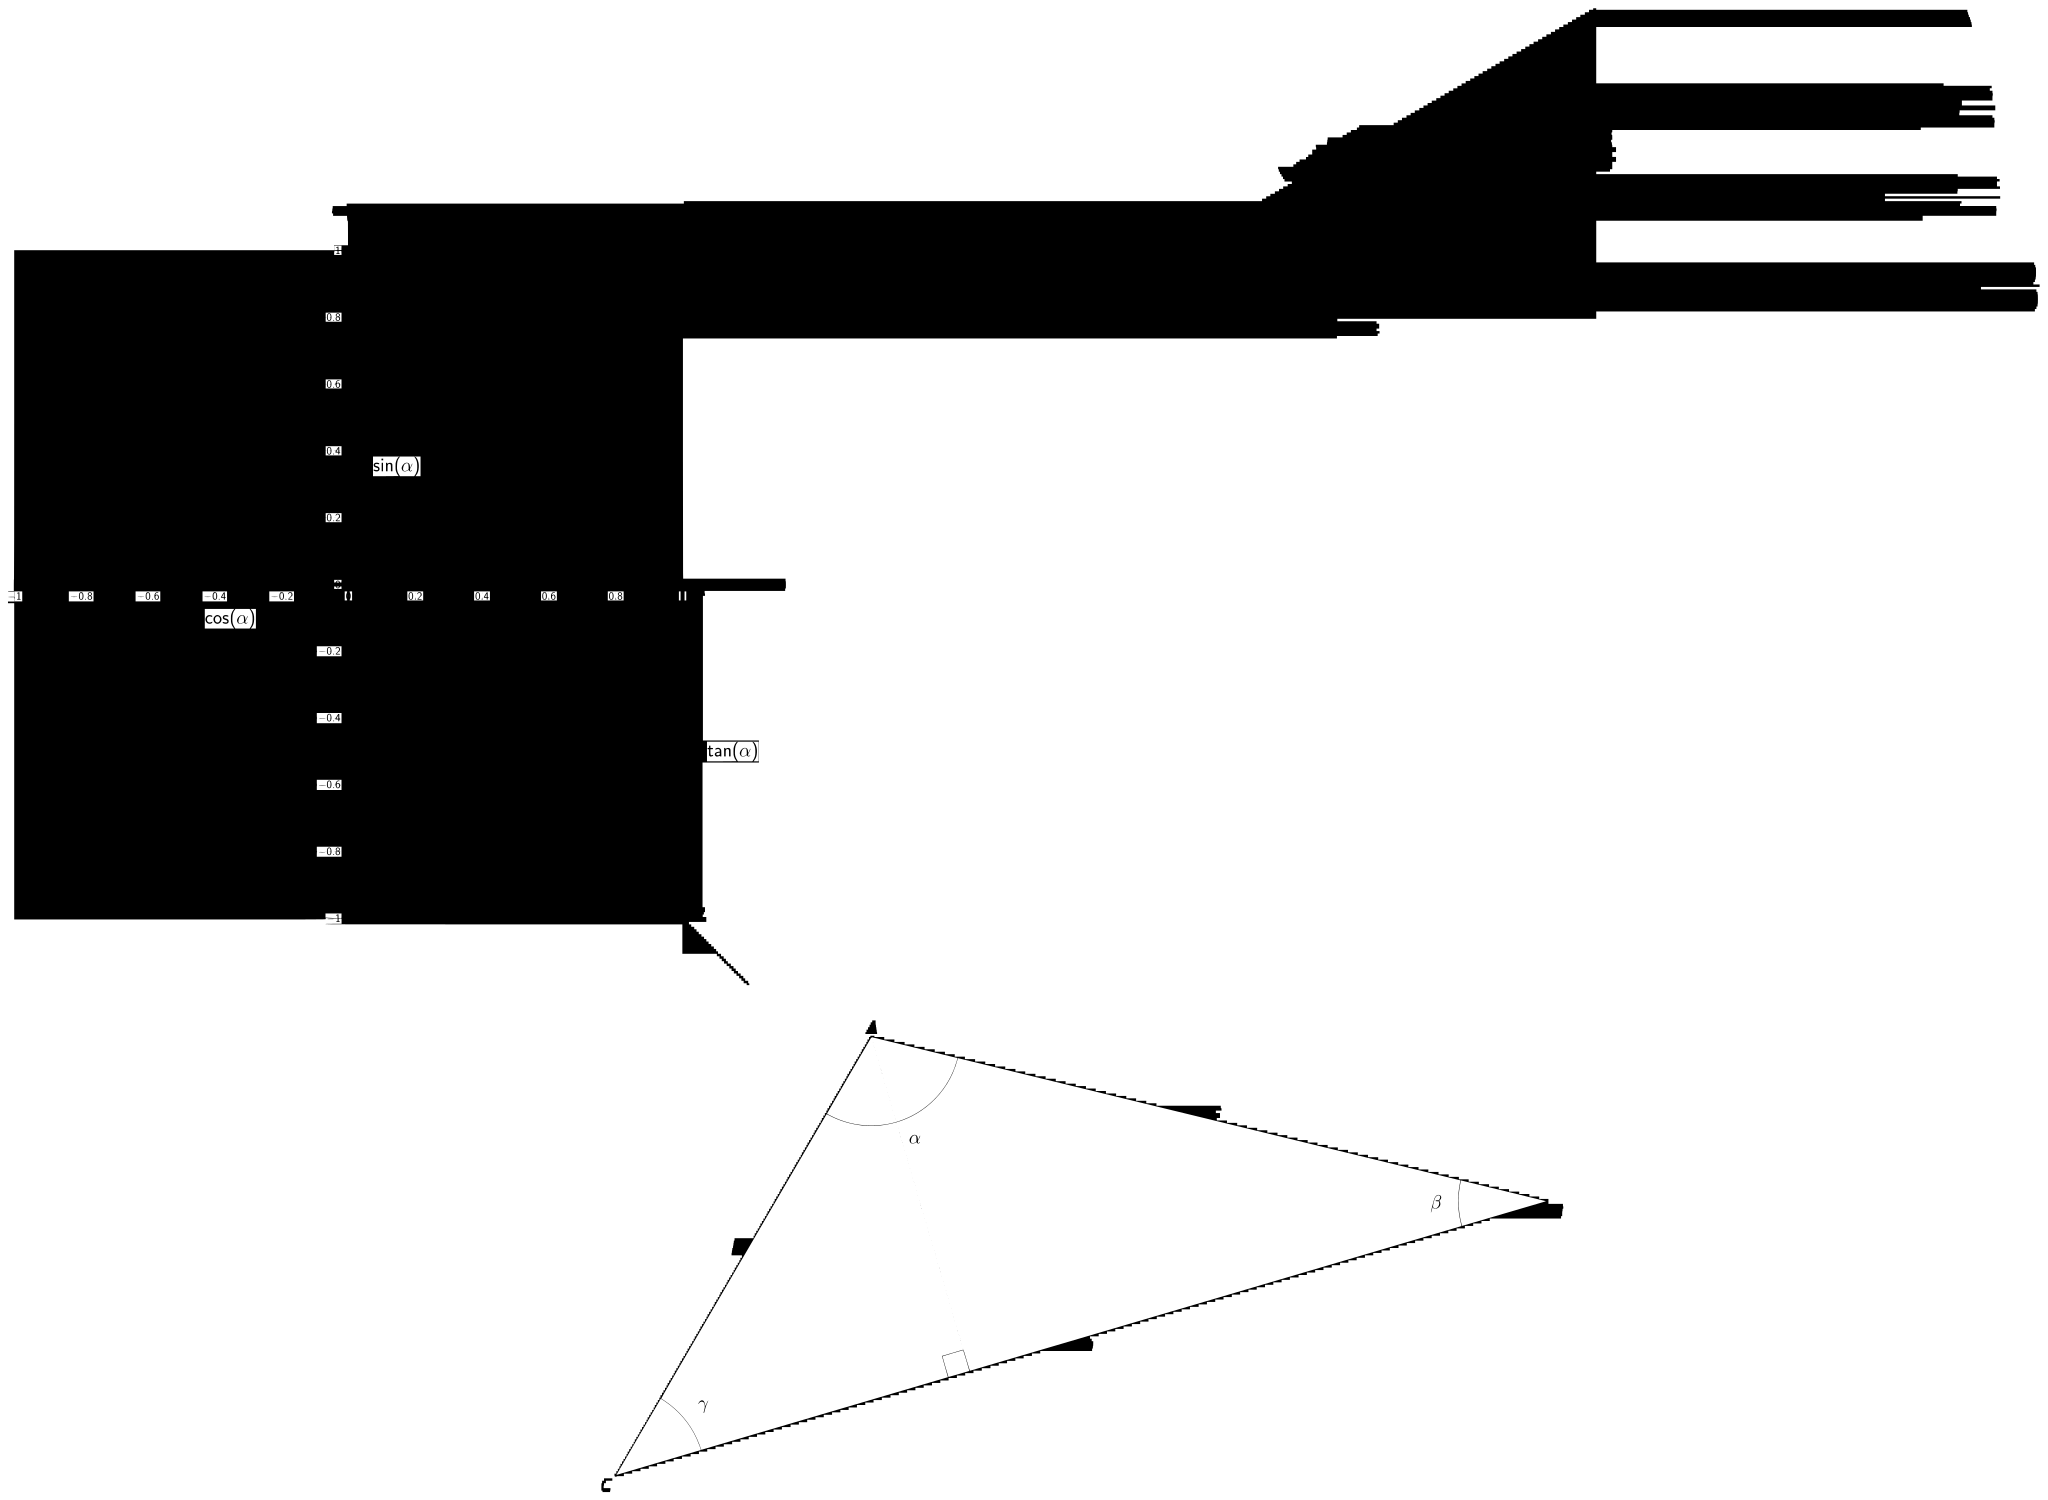
\includegraphics[width=\linewidth]{figures/fig1.pdf}\vspace{3cm}}
\KOMAoption{captions}{tableheading}
\makeatletter
\@ifpackageloaded{tcolorbox}{}{\usepackage[skins,breakable]{tcolorbox}}
\@ifpackageloaded{fontawesome5}{}{\usepackage{fontawesome5}}
\definecolor{quarto-callout-color}{HTML}{909090}
\definecolor{quarto-callout-note-color}{HTML}{0758E5}
\definecolor{quarto-callout-important-color}{HTML}{CC1914}
\definecolor{quarto-callout-warning-color}{HTML}{EB9113}
\definecolor{quarto-callout-tip-color}{HTML}{00A047}
\definecolor{quarto-callout-caution-color}{HTML}{FC5300}
\definecolor{quarto-callout-color-frame}{HTML}{acacac}
\definecolor{quarto-callout-note-color-frame}{HTML}{4582ec}
\definecolor{quarto-callout-important-color-frame}{HTML}{d9534f}
\definecolor{quarto-callout-warning-color-frame}{HTML}{f0ad4e}
\definecolor{quarto-callout-tip-color-frame}{HTML}{02b875}
\definecolor{quarto-callout-caution-color-frame}{HTML}{fd7e14}
\makeatother
\makeatletter
\@ifpackageloaded{bookmark}{}{\usepackage{bookmark}}
\makeatother
\makeatletter
\@ifpackageloaded{caption}{}{\usepackage{caption}}
\AtBeginDocument{%
\ifdefined\contentsname
  \renewcommand*\contentsname{Table des matières}
\else
  \newcommand\contentsname{Table des matières}
\fi
\ifdefined\listfigurename
  \renewcommand*\listfigurename{Liste des Figures}
\else
  \newcommand\listfigurename{Liste des Figures}
\fi
\ifdefined\listtablename
  \renewcommand*\listtablename{Liste des Tables}
\else
  \newcommand\listtablename{Liste des Tables}
\fi
\ifdefined\figurename
  \renewcommand*\figurename{Figure}
\else
  \newcommand\figurename{Figure}
\fi
\ifdefined\tablename
  \renewcommand*\tablename{Table}
\else
  \newcommand\tablename{Table}
\fi
}
\@ifpackageloaded{float}{}{\usepackage{float}}
\floatstyle{ruled}
\@ifundefined{c@chapter}{\newfloat{codelisting}{h}{lop}}{\newfloat{codelisting}{h}{lop}[chapter]}
\floatname{codelisting}{Listing}
\newcommand*\listoflistings{\listof{codelisting}{Liste des Listings}}
\usepackage{amsthm}
\theoremstyle{definition}
\newtheorem{definition}{Définition}[chapter]
\theoremstyle{definition}
\newtheorem{exercise}{Exercice}[chapter]
\theoremstyle{plain}
\newtheorem{theorem}{Théorème}[chapter]
\theoremstyle{definition}
\newtheorem{example}{Exemple}[chapter]
\theoremstyle{remark}
\AtBeginDocument{\renewcommand*{\proofname}{Preuve}}
\newtheorem*{remark}{Remarque}
\newtheorem*{solution}{Solution}
\newtheorem{refremark}{Remarque}[chapter]
\newtheorem{refsolution}{Solution}[chapter]
\makeatother
\makeatletter
\makeatother
\makeatletter
\@ifpackageloaded{caption}{}{\usepackage{caption}}
\@ifpackageloaded{subcaption}{}{\usepackage{subcaption}}
\makeatother
\newcounter{quartocalloutnteno}
\newcommand{\quartocalloutnte}[1]{\refstepcounter{quartocalloutnteno}\label{#1}}

\ifLuaTeX
\usepackage[bidi=basic]{babel}
\else
\usepackage[bidi=default]{babel}
\fi
\babelprovide[main,import]{french}
% get rid of language-specific shorthands (see #6817):
\let\LanguageShortHands\languageshorthands
\def\languageshorthands#1{}
\ifLuaTeX
  \usepackage{selnolig}  % disable illegal ligatures
\fi
\usepackage{bookmark}

\IfFileExists{xurl.sty}{\usepackage{xurl}}{} % add URL line breaks if available
\urlstyle{same} % disable monospaced font for URLs
\hypersetup{
  pdftitle={4UAA3: Trigonométrie},
  pdfauthor={Quentin Lambotte},
  pdflang={fr},
  colorlinks=true,
  linkcolor={blue},
  filecolor={Maroon},
  citecolor={Blue},
  urlcolor={Blue},
  pdfcreator={LaTeX via pandoc}}


\title{4UAA3: Trigonométrie}
\author{Quentin Lambotte}
\date{}

\begin{document}
\maketitle


\bookmarksetup{startatroot}

\chapter*{}\label{section}
\addcontentsline{toc}{chapter}{}

\markboth{}{}

\bookmarksetup{startatroot}

\chapter{Les triangles quelconques}\label{les-triangles-quelconques}

\section{Rappels: trigonométrie dans le triangle
rectangle}\label{rappels-trigonomuxe9trie-dans-le-triangle-rectangle}

Dans cette UAA, nous prendrons l'habitude d'annoter les triangles de la
manière suivante:

\begin{center}
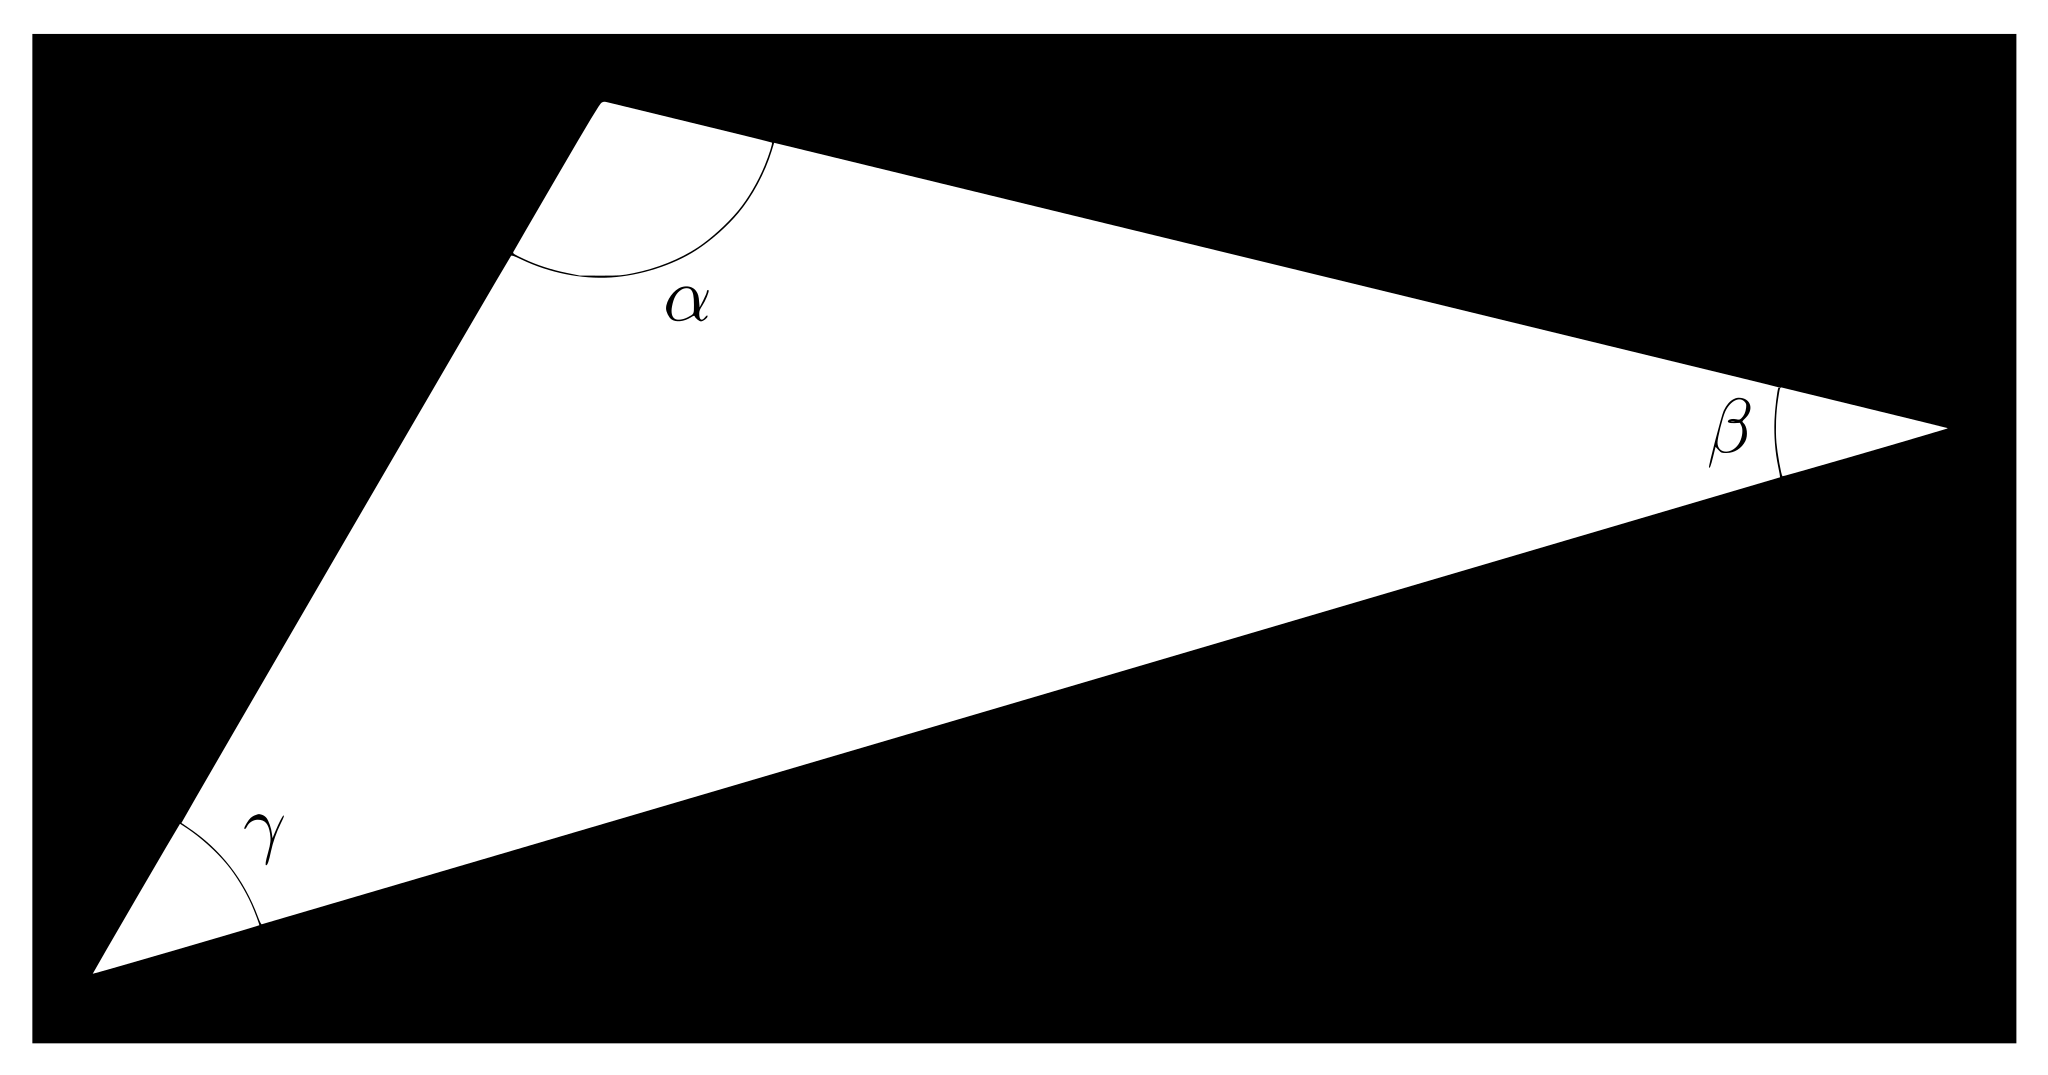
\includegraphics[width=0.45\textwidth,height=\textheight]{figures/fig2.pdf}
\end{center}

\begin{itemize}
\tightlist
\item
  chaque côté porte la lettre minuscule du sommet opposé
\item
  l'angle d'un sommet porte la lettre grècque correspondante.
\end{itemize}

Voici l'essentiel de la trigonométrie du triangle rectangle.

\begin{center}
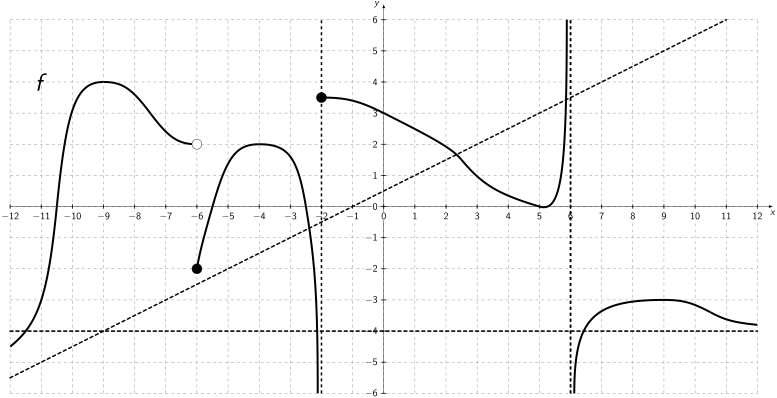
\includegraphics[width=0.8\textwidth,height=\textheight]{figures/fig3.pdf}
\end{center}

\begin{theorem}[]\protect\hypertarget{thm-pytagore}{}\label{thm-pytagore}

Dans un triangle \(ABC\) rectangle en \(A\), \(a^2=b^2+c^2\).

\begin{center}
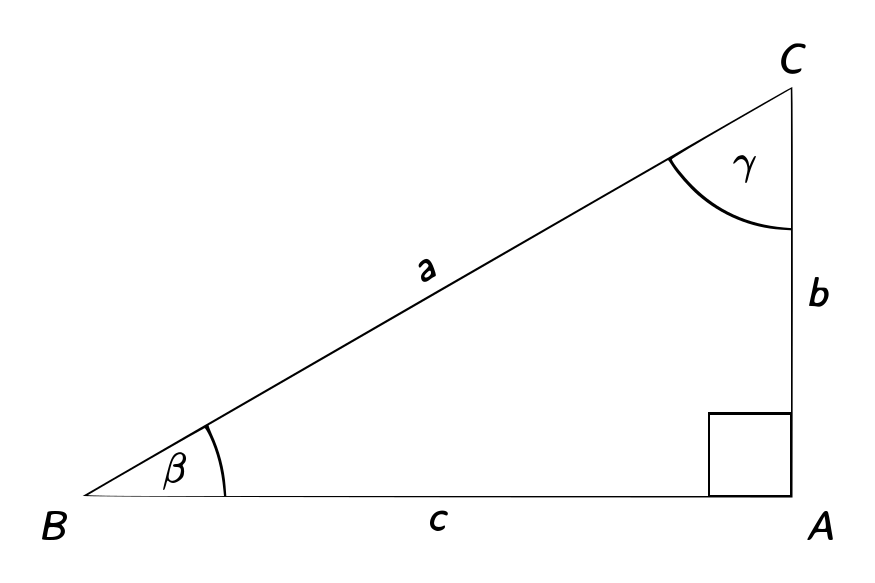
\includegraphics[width=0.45\textwidth,height=\textheight]{figures/fig5.pdf}
\end{center}

\end{theorem}

De plus, tu as vu dans le cours de 3e quelques valeurs particulières de
nombres trigonométriques

\begin{longtable}[]{@{}
  >{\raggedright\arraybackslash}p{(\columnwidth - 10\tabcolsep) * \real{0.1667}}
  >{\raggedright\arraybackslash}p{(\columnwidth - 10\tabcolsep) * \real{0.1667}}
  >{\raggedright\arraybackslash}p{(\columnwidth - 10\tabcolsep) * \real{0.1667}}
  >{\raggedright\arraybackslash}p{(\columnwidth - 10\tabcolsep) * \real{0.1667}}
  >{\raggedright\arraybackslash}p{(\columnwidth - 10\tabcolsep) * \real{0.1667}}
  >{\raggedright\arraybackslash}p{(\columnwidth - 10\tabcolsep) * \real{0.1667}}@{}}
\toprule\noalign{}
\begin{minipage}[b]{\linewidth}\raggedright
Mesure de l'angle \(\alpha\)
\end{minipage} & \begin{minipage}[b]{\linewidth}\raggedright
\(0^\circ\)
\end{minipage} & \begin{minipage}[b]{\linewidth}\raggedright
\(30^\circ\)
\end{minipage} & \begin{minipage}[b]{\linewidth}\raggedright
\(45^\circ\)
\end{minipage} & \begin{minipage}[b]{\linewidth}\raggedright
\(60^\circ\)
\end{minipage} & \begin{minipage}[b]{\linewidth}\raggedright
\(90^\circ\)
\end{minipage} \\
\midrule\noalign{}
\endhead
\bottomrule\noalign{}
\endlastfoot
\(\sin(\alpha)\) & 0 & \(\dfrac{1}{2}\) & \(\dfrac{\sqrt{2}}{2}\) &
\(\dfrac{\sqrt{3}}{2}\) & \(1\) \\
\(\cos(\alpha)\) & 1 & \(\dfrac{\sqrt{3}}{2}\) & \(\dfrac{\sqrt{2}}{2}\)
& \(\dfrac{1}{2}\) & 0 \\
\(\tan(\alpha)\) & 0 & \(\dfrac{\sqrt{3}}{3}\) & 1 & \(\sqrt{3}\) &
n'existe pas \\
\end{longtable}

\begin{exercise}[]\protect\hypertarget{exr-trig}{}\label{exr-trig}

Voici un triangle rectangle. Complète les égalités demandées.

\begin{center}
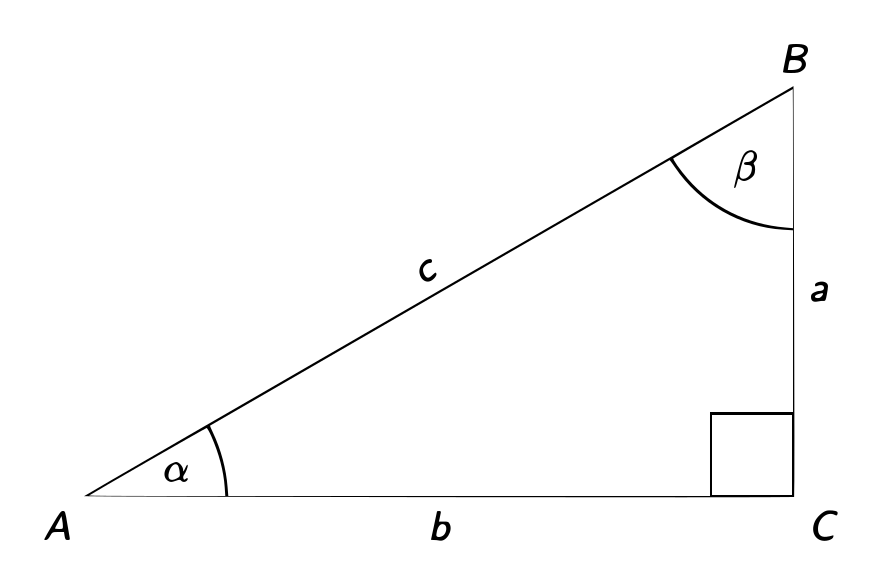
\includegraphics[width=0.45\textwidth,height=\textheight]{figures/fig4.pdf}
\end{center}

\begin{figure}

\begin{minipage}{0.50\linewidth}

\begin{enumerate}
\def\labelenumi{\roman{enumi})}
\item
  \(\sin(\alpha)=\)\dotfill
\item
  \(\cos(\alpha)=\)\dotfill
\item
  \(\tan(\alpha)=\)\dotfill
\end{enumerate}

\end{minipage}%
%
\begin{minipage}{0.50\linewidth}

\begin{enumerate}
\def\labelenumi{\roman{enumi})}
\item
  \(\sin(\beta)=\)\dotfill
\item
  \(\cos(\beta)=\)\dotfill
\item
  \(\tan(\beta)=\)\dotfill
\end{enumerate}

\end{minipage}%

\end{figure}%

\end{exercise}

\begin{exercise}[]\protect\hypertarget{exr-hauteur}{}\label{exr-hauteur}

Soit \(ABC\) un triangle rectangle en \(C\). On sait que l'hypothénuse
mesure \(11\) cm et que l'angle \(\alpha\) mesure \(35^\circ\).

\begin{center}
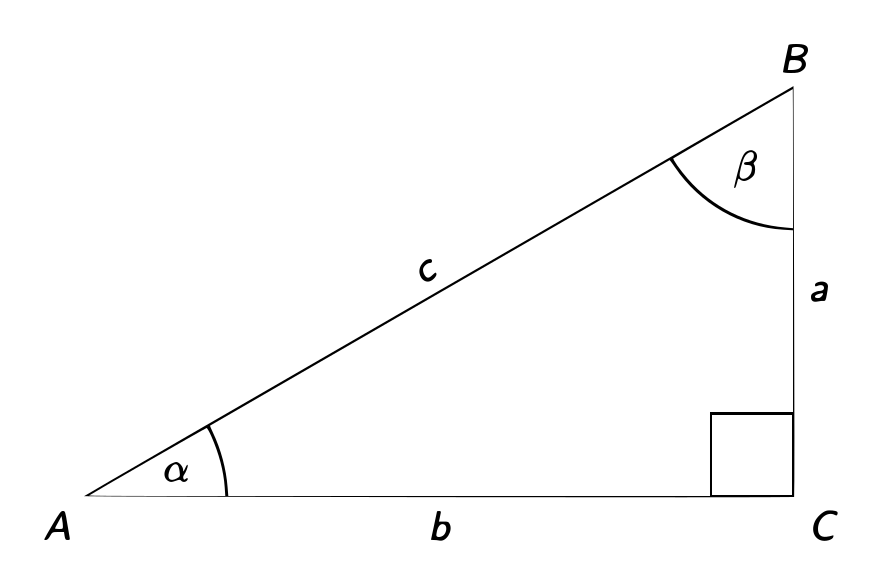
\includegraphics[width=0.45\textwidth,height=\textheight]{figures/fig4.pdf}
\end{center}

\begin{itemize}
\tightlist
\item
  complète l'égalité suivante: \(\sin(\alpha)=\)\dotfill.
\item
  calcule à l'aide de la formule précédente la longueur du côté \(a\).
\end{itemize}

\end{exercise}

\begin{exercise}[]\protect\hypertarget{exr-calculs}{}\label{exr-calculs}

Soit \(ABC\) un triangle rectangle en \(A\). On suppose que
\(\overline{AB}=4\)cm et \(\overline{AC}=7\).

\begin{center}
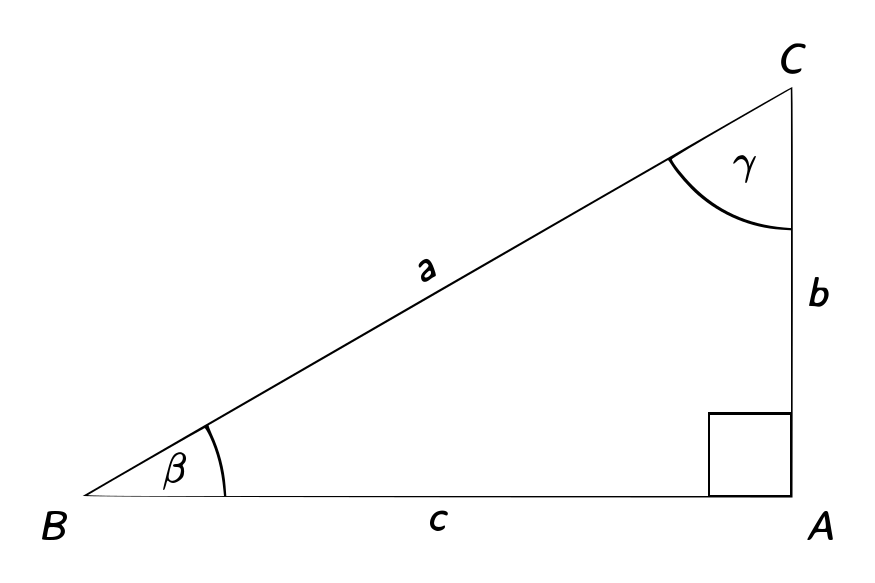
\includegraphics[width=0.45\textwidth,height=\textheight]{figures/fig5.pdf}
\end{center}

\begin{itemize}
\tightlist
\item
  calcule la longeur du côté \(\overline{BC}\).
\item
  calcule l'angle \(\beta\).
\end{itemize}

\end{exercise}

\section{Aire d'un triangle
quelconque}\label{aire-dun-triangle-quelconque}

En te basant sur la trigonométrie du triangle rectangle, tu vas essayer
de découvrir une nouvelle formule pour calculer l'aire d'un triangle
quelconque.

\begin{exercise}[]\protect\hypertarget{exr-1}{}\label{exr-1}

Soit \(ABC\) le triangle dont le côté \(b\) mesure 5cm, le côté \(a\)
mesure 6cm et tel \(\gamma=45^\circ\).

\begin{enumerate}
\def\labelenumi{\arabic{enumi}.}
\tightlist
\item
  Trace le triangle \(ABC\) avec précision.
\item
  À l'aide du dessin, estime l'aire du triangle \(ABC\).
\item
  Calcule l'aire du triangle \(ABC\).
\end{enumerate}

\end{exercise}

\begin{exercise}[]\protect\hypertarget{exr-2}{}\label{exr-2}

Fais le même exercice pour le triangle \(ABC\) dont le côté \(c\) mesure
8cm, le côté \(b\) mesure 8cm et tel que \(\alpha=30^\circ\).

\end{exercise}

\begin{theorem}[]\protect\hypertarget{thm-aire}{}\label{thm-aire}

Étant donné un triangle \(ABC\), on peut calculer l'aire de ce triangle
grâce à la formule: \(\text{Aire}(ABC)=\)\dotfill

\end{theorem}

\begin{tcolorbox}[enhanced jigsaw, breakable, colback=white, arc=.35mm, left=2mm, toprule=.15mm, rightrule=.15mm, leftrule=.75mm, colframe=quarto-callout-note-color-frame, bottomrule=.15mm, opacityback=0]

\quartocalloutnte{nte-idee} 

\vspace{-3mm}\textbf{Note \ref*{nte-idee}: Remarque}\vspace{3mm}

Quelle est l'idée qui a permis de construire la formule du calcul
d'aire? \vspace{4cm}

\end{tcolorbox}

\newpage

\section{Lois des sinus et cosinus}\label{lois-des-sinus-et-cosinus}

\begin{enumerate}
\def\labelenumi{\arabic{enumi})}
\tightlist
\item
  Soit \(ABC\) un triangle tel que \(\alpha=80^\circ\),
  \(\gamma=60^\circ\) et \(b=\) 3cm. Nous allons essayer de compléter le
  tableau suivant:
\end{enumerate}

\begin{longtable}[]{@{}
  >{\raggedright\arraybackslash}p{(\columnwidth - 12\tabcolsep) * \real{0.1000}}
  >{\raggedright\arraybackslash}p{(\columnwidth - 12\tabcolsep) * \real{0.1000}}
  >{\raggedright\arraybackslash}p{(\columnwidth - 12\tabcolsep) * \real{0.1000}}
  >{\raggedright\arraybackslash}p{(\columnwidth - 12\tabcolsep) * \real{0.2000}}
  >{\raggedright\arraybackslash}p{(\columnwidth - 12\tabcolsep) * \real{0.1800}}
  >{\raggedright\arraybackslash}p{(\columnwidth - 12\tabcolsep) * \real{0.2000}}
  >{\raggedright\arraybackslash}p{(\columnwidth - 12\tabcolsep) * \real{0.1200}}@{}}
\toprule\noalign{}
\begin{minipage}[b]{\linewidth}\raggedright
\(a\)
\end{minipage} & \begin{minipage}[b]{\linewidth}\raggedright
\(b\)
\end{minipage} & \begin{minipage}[b]{\linewidth}\raggedright
\(c\)
\end{minipage} & \begin{minipage}[b]{\linewidth}\raggedright
\(\alpha\)
\end{minipage} & \begin{minipage}[b]{\linewidth}\raggedright
\(\beta\)
\end{minipage} & \begin{minipage}[b]{\linewidth}\raggedright
\(\gamma\)
\end{minipage} & \begin{minipage}[b]{\linewidth}\raggedright
Aire
\end{minipage} \\
\midrule\noalign{}
\endhead
\bottomrule\noalign{}
\endlastfoot
& 3 & & \(80^\circ\) & & \(60^\circ\) & \\
\end{longtable}

\begin{exercise}[]\protect\hypertarget{exr-loi-sin-1}{}\label{exr-loi-sin-1}

~

\begin{enumerate}
\def\labelenumi{\arabic{enumi}.}
\tightlist
\item
  Trace le triangle demandé à l'échelle.
\item
  Complète le tableau suivant estimant les valeurs manquantes:
\end{enumerate}

\begin{longtable}[]{@{}
  >{\raggedright\arraybackslash}p{(\columnwidth - 14\tabcolsep) * \real{0.2063}}
  >{\raggedright\arraybackslash}p{(\columnwidth - 14\tabcolsep) * \real{0.0794}}
  >{\raggedright\arraybackslash}p{(\columnwidth - 14\tabcolsep) * \real{0.0794}}
  >{\raggedright\arraybackslash}p{(\columnwidth - 14\tabcolsep) * \real{0.0794}}
  >{\raggedright\arraybackslash}p{(\columnwidth - 14\tabcolsep) * \real{0.1587}}
  >{\raggedright\arraybackslash}p{(\columnwidth - 14\tabcolsep) * \real{0.1429}}
  >{\raggedright\arraybackslash}p{(\columnwidth - 14\tabcolsep) * \real{0.1587}}
  >{\raggedright\arraybackslash}p{(\columnwidth - 14\tabcolsep) * \real{0.0952}}@{}}
\toprule\noalign{}
\begin{minipage}[b]{\linewidth}\raggedright
\end{minipage} & \begin{minipage}[b]{\linewidth}\raggedright
\(a\)
\end{minipage} & \begin{minipage}[b]{\linewidth}\raggedright
\(b\)
\end{minipage} & \begin{minipage}[b]{\linewidth}\raggedright
\(c\)
\end{minipage} & \begin{minipage}[b]{\linewidth}\raggedright
\(\alpha\)
\end{minipage} & \begin{minipage}[b]{\linewidth}\raggedright
\(\beta\)
\end{minipage} & \begin{minipage}[b]{\linewidth}\raggedright
\(\gamma\)
\end{minipage} & \begin{minipage}[b]{\linewidth}\raggedright
Aire
\end{minipage} \\
\midrule\noalign{}
\endhead
\bottomrule\noalign{}
\endlastfoot
Estimations & & 3 & & \(80^\circ\) & & \(60^\circ\) & \\
\end{longtable}

\end{exercise}

\begin{exercise}[]\protect\hypertarget{exr-loi-sin}{}\label{exr-loi-sin}

~

\begin{enumerate}
\def\labelenumi{\arabic{enumi}.}
\tightlist
\item
  Quelle est la mesure de l'angle \(\beta\)?
\item
  Écris les formules de l'aire pour \(ABC\).
\item
  A partir de ces formules, trouve la mesure du côté \(a\).
\item
  Trouve ensuite la mesure du côté \(c\).
\end{enumerate}

\end{exercise}

\begin{theorem}[Loi des
sinus]\protect\hypertarget{thm-aire}{}\label{thm-aire}

Étant donné un triangle \(ABC\), \vspace{2cm}

\end{theorem}

\begin{enumerate}
\def\labelenumi{\arabic{enumi})}
\setcounter{enumi}{1}
\tightlist
\item
  Soit \(ABC\) un triangle tel que \(\alpha=60^\circ\), \(c=5\) cm et
  \(b=\) 4cm. Nous allons essayer de compléter le tableau suivant:
\end{enumerate}

\begin{longtable}[]{@{}
  >{\raggedright\arraybackslash}p{(\columnwidth - 10\tabcolsep) * \real{0.1136}}
  >{\raggedright\arraybackslash}p{(\columnwidth - 10\tabcolsep) * \real{0.1136}}
  >{\raggedright\arraybackslash}p{(\columnwidth - 10\tabcolsep) * \real{0.1136}}
  >{\raggedright\arraybackslash}p{(\columnwidth - 10\tabcolsep) * \real{0.2273}}
  >{\raggedright\arraybackslash}p{(\columnwidth - 10\tabcolsep) * \real{0.2045}}
  >{\raggedright\arraybackslash}p{(\columnwidth - 10\tabcolsep) * \real{0.2273}}@{}}
\toprule\noalign{}
\begin{minipage}[b]{\linewidth}\raggedright
\(a\)
\end{minipage} & \begin{minipage}[b]{\linewidth}\raggedright
\(b\)
\end{minipage} & \begin{minipage}[b]{\linewidth}\raggedright
\(c\)
\end{minipage} & \begin{minipage}[b]{\linewidth}\raggedright
\(\alpha\)
\end{minipage} & \begin{minipage}[b]{\linewidth}\raggedright
\(\beta\)
\end{minipage} & \begin{minipage}[b]{\linewidth}\raggedright
\(\gamma\)
\end{minipage} \\
\midrule\noalign{}
\endhead
\bottomrule\noalign{}
\endlastfoot
{\phantom{zùerokzùemrlk}} & 4 & 5 & \(60^\circ\) & & \\
\end{longtable}

\begin{exercise}[]\protect\hypertarget{exr-loi-sin-1}{}\label{exr-loi-sin-1}

~

\begin{enumerate}
\def\labelenumi{\arabic{enumi}.}
\tightlist
\item
  Trace le triangle demandé à l'échelle. Fais en sorte que le côté \(b\)
  soit horizontal et que l'angle \(\alpha\) soit à l'extrémité gauche de
  \(b\).
\item
  Complète le tableau suivant estimant les valeurs manquantes:
\end{enumerate}

\begin{longtable}[]{@{}
  >{\raggedright\arraybackslash}p{(\columnwidth - 12\tabcolsep) * \real{0.2281}}
  >{\raggedright\arraybackslash}p{(\columnwidth - 12\tabcolsep) * \real{0.0877}}
  >{\raggedright\arraybackslash}p{(\columnwidth - 12\tabcolsep) * \real{0.0877}}
  >{\raggedright\arraybackslash}p{(\columnwidth - 12\tabcolsep) * \real{0.0877}}
  >{\raggedright\arraybackslash}p{(\columnwidth - 12\tabcolsep) * \real{0.1754}}
  >{\raggedright\arraybackslash}p{(\columnwidth - 12\tabcolsep) * \real{0.1579}}
  >{\raggedright\arraybackslash}p{(\columnwidth - 12\tabcolsep) * \real{0.1754}}@{}}
\toprule\noalign{}
\begin{minipage}[b]{\linewidth}\raggedright
\end{minipage} & \begin{minipage}[b]{\linewidth}\raggedright
\(a\)
\end{minipage} & \begin{minipage}[b]{\linewidth}\raggedright
\(b\)
\end{minipage} & \begin{minipage}[b]{\linewidth}\raggedright
\(c\)
\end{minipage} & \begin{minipage}[b]{\linewidth}\raggedright
\(\alpha\)
\end{minipage} & \begin{minipage}[b]{\linewidth}\raggedright
\(\beta\)
\end{minipage} & \begin{minipage}[b]{\linewidth}\raggedright
\(\gamma\)
\end{minipage} \\
\midrule\noalign{}
\endhead
\bottomrule\noalign{}
\endlastfoot
Estimations & & 4 & 5 & \(60^\circ\) & & \\
\end{longtable}

\end{exercise}

\begin{exercise}[]\protect\hypertarget{exr-loi-sin}{}\label{exr-loi-sin}

~

\begin{enumerate}
\def\labelenumi{\arabic{enumi}.}
\tightlist
\item
  Trace la hauteur \(h\) passant par \(B\).
\item
  Note \(H\) le point d'intersection entre la hauteur \(h\) et le côté
  \(b\).
\item
  Note \(b'\) le segment \([AH]\) et \(b''\) le segment \(HC\).
\item
  Tu obtiens deux triangles rectangles: \(ABH\) et \(CBH\). Écris pour
  ceux deux triangles le théorème de Pythagore.
\item
  Utilises ces deux formules et le fait que \(b=b'+b''\) pour trouver la
  mesure du côté \(a\).
\end{enumerate}

\end{exercise}

\begin{theorem}[Loi des cosinus ou théorème de Pythagore
généralisé]\protect\hypertarget{thm-aire}{}\label{thm-aire}

Étant donné un triangle \(ABC\), \vspace{2cm}

\end{theorem}

\newpage

\subsection{Construction de la loi des consinus par généralisation
algébrique}\label{construction-de-la-loi-des-consinus-par-guxe9nuxe9ralisation-alguxe9brique}

\begin{longtable}[]{@{}
  >{\raggedright\arraybackslash}p{(\columnwidth - 2\tabcolsep) * \real{0.4828}}
  >{\raggedright\arraybackslash}p{(\columnwidth - 2\tabcolsep) * \real{0.5172}}@{}}
\toprule\noalign{}
\begin{minipage}[b]{\linewidth}\raggedright
Exemple algébrique
\end{minipage} & \begin{minipage}[b]{\linewidth}\raggedright
Généralisation
\end{minipage} \\
\midrule\noalign{}
\endhead
\bottomrule\noalign{}
\endlastfoot
\begin{center}
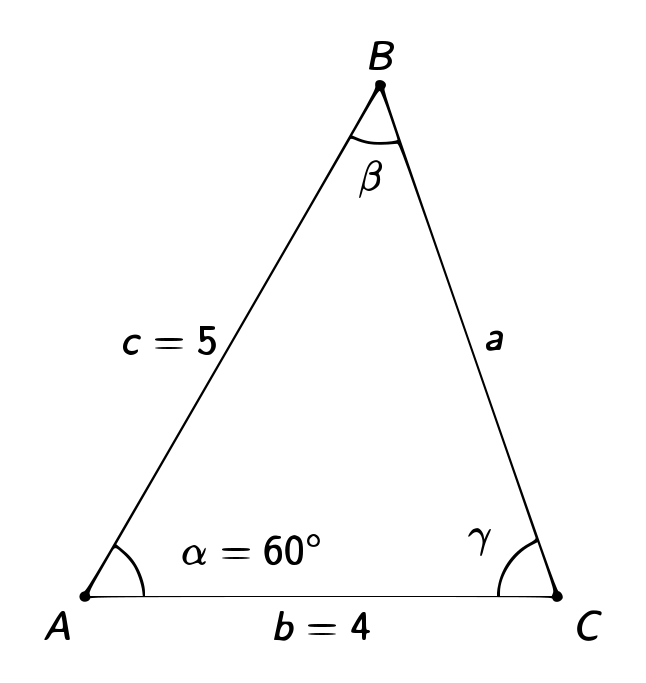
\includegraphics[width=0.25\textwidth,height=\textheight]{figures/fig6.pdf}
\end{center}
& \begin{center}
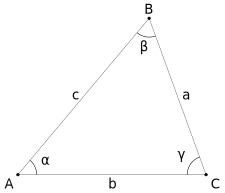
\includegraphics[width=0.3\textwidth,height=\textheight]{figures/triangle.pdf}
\end{center}
 \\
\multicolumn{2}{@{}>{\raggedright\arraybackslash}p{(\columnwidth - 2\tabcolsep) * \real{1.0000} + 2\tabcolsep}@{}}{%
\begin{minipage}[t]{\linewidth}\raggedright
\begin{center}
Étape 1: \ul{Tracé de la hauteur $h$ passant par $B$}

\end{center}
\end{minipage}} \\
& \\
\multicolumn{2}{@{}>{\raggedright\arraybackslash}p{(\columnwidth - 2\tabcolsep) * \real{1.0000} + 2\tabcolsep}@{}}{%
\begin{minipage}[t]{\linewidth}\raggedright
\begin{itemize}
\tightlist
\item
  \(H\) est l'intersection de \(h\) avec \(b\)
\item
  \(b'\) est le segment \([AH]\) et \(b''\) le segment \([HC]\)
\item
  les triangles \(ABH\) et \(HBC\) sont rectangles
\end{itemize}
\end{minipage}} \\
& \\
\multicolumn{2}{@{}>{\raggedright\arraybackslash}p{(\columnwidth - 2\tabcolsep) * \real{1.0000} + 2\tabcolsep}@{}}{%
\begin{minipage}[t]{\linewidth}\raggedright
\begin{center}
Étape 2: \ul{On applique le théorème de Pythagore aux deux triangles
rectangles $ABH$ et $HBC$.}

\end{center}
\end{minipage}} \\
& \\
\begin{minipage}[t]{\linewidth}\raggedright
\begin{itemize}
\tightlist
\item
  pour \(ABH\) : \(5^2=h^2+b'^2\)
\item
  pour \(HBC\) : \(a^2=h^2+b''^2\)
\end{itemize}
\end{minipage} & \begin{minipage}[t]{\linewidth}\raggedright
\begin{itemize}
\tightlist
\item
  pour \(ABH\) : \(c^2=h^2+b'^2\)
\item
  pour \(HBC\) : \(a^2=h^2+b''^2\)
\end{itemize}
\end{minipage} \\
\multicolumn{2}{@{}>{\raggedright\arraybackslash}p{(\columnwidth - 2\tabcolsep) * \real{1.0000} + 2\tabcolsep}@{}}{%
} \\
\multicolumn{2}{@{}>{\raggedright\arraybackslash}p{(\columnwidth - 2\tabcolsep) * \real{1.0000} + 2\tabcolsep}@{}}{%
\begin{minipage}[t]{\linewidth}\raggedright
\begin{center}
Étape 3: \ul{On utilise les deux formules et le fait que $b=b'+b''$ pour
trouver $a$.}

\end{center}
\end{minipage}} \\
& \\
\begin{minipage}[t]{\linewidth}\raggedright
\begin{itemize}
\tightlist
\item
  \(h^2= 25-b'^2\)
\item
  \(b''=4-b'\)
\end{itemize}
\end{minipage} & \begin{minipage}[t]{\linewidth}\raggedright
\begin{itemize}
\tightlist
\item
  puisque \(c^2=h^2+b'^2\), on a que \(h^2=\makebox[2cm]{\dotfill}\)
\item
  puisque \(b=b'+b''\), on a que \(b''=\makebox[2cm]{\dotfill}\)
\end{itemize}
\end{minipage} \\
Donc

\(
 \begin{aligned}
a^2&=h^2+b''^2\\
&=25-b'^2+(4-b')^2\\
&=25-b'^2+4^2-2\cdot 4b'+b'^2\\
&=25+16-2\cdot 4b'
\end{aligned}
\)

Or, \(\cos(\alpha)=\dfrac{b'}{5}\).

Donc \(b'=5\cos(60)=5\dfrac{\sqrt{3}}{2}\)

Et donc

\(a^2=41-8\cdot 5\dfrac{1}{2}=41-20\).

Donc \(a=\sqrt{21}\). & Donc:

\(
\begin{aligned}
a^2&=h^2+b''^2\\
&=c^2-b'^2+(b-b')^2\\
&=c^2-b'^2+b^2-2bb'+b'^2\\
&=c^2+b^2-2bb'
\end{aligned}
\)

Or, \(\cos(\alpha)=\makebox[3cm]{\dotfill}\).

Donc \(b'=\makebox[3cm]{\dotfill}\).

Et donc \(
a^2=c^2+b^2-2bc\cos(\alpha).
\) \\
\end{longtable}

\section{Exercices}\label{exercices}

Pour les exercices suivants, on travaille avec des triangles respectant
les notations suivantes:

\begin{center}
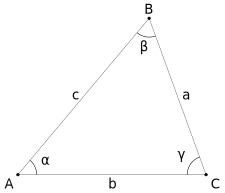
\includegraphics[width=0.45\textwidth,height=\textheight]{figures/triangle.pdf}
\end{center}

\begin{exercise}[]\protect\hypertarget{exr-calcul-aire}{}\label{exr-calcul-aire}

À l'aide de la loi des aires, calcule l'aire des triangles suivants à
partir des données fournies (arrondis à \(10^{-3}\) près).

\begin{longtable}[]{@{}
  >{\raggedright\arraybackslash}p{(\columnwidth - 12\tabcolsep) * \real{0.0806}}
  >{\raggedright\arraybackslash}p{(\columnwidth - 12\tabcolsep) * \real{0.0806}}
  >{\raggedright\arraybackslash}p{(\columnwidth - 12\tabcolsep) * \real{0.0806}}
  >{\raggedright\arraybackslash}p{(\columnwidth - 12\tabcolsep) * \real{0.1613}}
  >{\raggedright\arraybackslash}p{(\columnwidth - 12\tabcolsep) * \real{0.1452}}
  >{\raggedright\arraybackslash}p{(\columnwidth - 12\tabcolsep) * \real{0.1613}}
  >{\raggedright\arraybackslash}p{(\columnwidth - 12\tabcolsep) * \real{0.2903}}@{}}
\toprule\noalign{}
\begin{minipage}[b]{\linewidth}\raggedright
\(a\)
\end{minipage} & \begin{minipage}[b]{\linewidth}\raggedright
\(b\)
\end{minipage} & \begin{minipage}[b]{\linewidth}\raggedright
\(c\)
\end{minipage} & \begin{minipage}[b]{\linewidth}\raggedright
\(\alpha\)
\end{minipage} & \begin{minipage}[b]{\linewidth}\raggedright
\(\beta\)
\end{minipage} & \begin{minipage}[b]{\linewidth}\raggedright
\(\gamma\)
\end{minipage} & \begin{minipage}[b]{\linewidth}\raggedright
Aire du triangle
\end{minipage} \\
\midrule\noalign{}
\endhead
\bottomrule\noalign{}
\endlastfoot
6 & 15 & & & & 46 & \\
& 50 & 12 & 10 & & & {\phantom{zùerokzùemrlk}} \\
3 & & 7,5 & & 26 & & \\
\end{longtable}

\end{exercise}

\begin{exercise}[]\protect\hypertarget{exr-applic-sinus}{}\label{exr-applic-sinus}

À l'aide de la loi des sinus, calcule l'élément demandé à partir des
mesures données dans le tableau (arrondis à \(10^{-3}\) près).

\begin{longtable}[]{@{}
  >{\raggedright\arraybackslash}p{(\columnwidth - 12\tabcolsep) * \real{0.0769}}
  >{\raggedright\arraybackslash}p{(\columnwidth - 12\tabcolsep) * \real{0.0769}}
  >{\raggedright\arraybackslash}p{(\columnwidth - 12\tabcolsep) * \real{0.0769}}
  >{\raggedright\arraybackslash}p{(\columnwidth - 12\tabcolsep) * \real{0.1538}}
  >{\raggedright\arraybackslash}p{(\columnwidth - 12\tabcolsep) * \real{0.1385}}
  >{\raggedright\arraybackslash}p{(\columnwidth - 12\tabcolsep) * \real{0.1538}}
  >{\raggedright\arraybackslash}p{(\columnwidth - 12\tabcolsep) * \real{0.3231}}@{}}
\toprule\noalign{}
\begin{minipage}[b]{\linewidth}\raggedright
\(a\)
\end{minipage} & \begin{minipage}[b]{\linewidth}\raggedright
\(b\)
\end{minipage} & \begin{minipage}[b]{\linewidth}\raggedright
\(c\)
\end{minipage} & \begin{minipage}[b]{\linewidth}\raggedright
\(\alpha\)
\end{minipage} & \begin{minipage}[b]{\linewidth}\raggedright
\(\beta\)
\end{minipage} & \begin{minipage}[b]{\linewidth}\raggedright
\(\gamma\)
\end{minipage} & \begin{minipage}[b]{\linewidth}\raggedright
Élément à calculer
\end{minipage} \\
\midrule\noalign{}
\endhead
\bottomrule\noalign{}
\endlastfoot
6 & & & 50 & 60 & & \(b\) \\
& 50 & & 10 & 30 & & \(a\) \\
3 & & 7,5 & 15 & & & \(\gamma\) \\
\end{longtable}

\end{exercise}

\begin{exercise}[]\protect\hypertarget{exr-applic-cos}{}\label{exr-applic-cos}

À l'aide de la loi des cosinus, calcule l'élément demandé à partir des
mesures données dans le tableau (arrondis à \(10^{-3}\) près).

\begin{longtable}[]{@{}
  >{\raggedright\arraybackslash}p{(\columnwidth - 12\tabcolsep) * \real{0.0769}}
  >{\raggedright\arraybackslash}p{(\columnwidth - 12\tabcolsep) * \real{0.0769}}
  >{\raggedright\arraybackslash}p{(\columnwidth - 12\tabcolsep) * \real{0.0769}}
  >{\raggedright\arraybackslash}p{(\columnwidth - 12\tabcolsep) * \real{0.1538}}
  >{\raggedright\arraybackslash}p{(\columnwidth - 12\tabcolsep) * \real{0.1385}}
  >{\raggedright\arraybackslash}p{(\columnwidth - 12\tabcolsep) * \real{0.1538}}
  >{\raggedright\arraybackslash}p{(\columnwidth - 12\tabcolsep) * \real{0.3231}}@{}}
\toprule\noalign{}
\begin{minipage}[b]{\linewidth}\raggedright
\(a\)
\end{minipage} & \begin{minipage}[b]{\linewidth}\raggedright
\(b\)
\end{minipage} & \begin{minipage}[b]{\linewidth}\raggedright
\(c\)
\end{minipage} & \begin{minipage}[b]{\linewidth}\raggedright
\(\alpha\)
\end{minipage} & \begin{minipage}[b]{\linewidth}\raggedright
\(\beta\)
\end{minipage} & \begin{minipage}[b]{\linewidth}\raggedright
\(\gamma\)
\end{minipage} & \begin{minipage}[b]{\linewidth}\raggedright
Élément à calculer
\end{minipage} \\
\midrule\noalign{}
\endhead
\bottomrule\noalign{}
\endlastfoot
7 & 8 & 10 & & & & \(\gamma\) \\
& 50 & 55 & 60 & & & \(a\) \\
3 & & 7,5 & & 15 & & \(b\) \\
\end{longtable}

\end{exercise}

Pour les exercices suivants, c'est à toi de déterminer quelle(s)
formule(s) à utiliser pour trouver toutes les mesures manquantes.

\begin{exercise}[]\protect\hypertarget{exr-resol-triangles}{}\label{exr-resol-triangles}

Soit \(ABC\) un triangle. Pour chacun des cas suivants, construis la
situation à l'aide de tes instruments, estime les mesures manquantes
puis détermine par calcul ces mesures (arrondis ta réponse finale au
centième).

\begin{enumerate}
\def\labelenumi{\arabic{enumi}.}
\tightlist
\item
  Premier cas: on connaît deux angles et un côté.
\end{enumerate}

\begin{longtable}[]{@{}
  >{\raggedright\arraybackslash}p{(\columnwidth - 10\tabcolsep) * \real{0.1136}}
  >{\raggedright\arraybackslash}p{(\columnwidth - 10\tabcolsep) * \real{0.1136}}
  >{\raggedright\arraybackslash}p{(\columnwidth - 10\tabcolsep) * \real{0.1136}}
  >{\raggedright\arraybackslash}p{(\columnwidth - 10\tabcolsep) * \real{0.2273}}
  >{\raggedright\arraybackslash}p{(\columnwidth - 10\tabcolsep) * \real{0.2045}}
  >{\raggedright\arraybackslash}p{(\columnwidth - 10\tabcolsep) * \real{0.2273}}@{}}
\toprule\noalign{}
\begin{minipage}[b]{\linewidth}\raggedright
\(a\)
\end{minipage} & \begin{minipage}[b]{\linewidth}\raggedright
\(b\)
\end{minipage} & \begin{minipage}[b]{\linewidth}\raggedright
\(c\)
\end{minipage} & \begin{minipage}[b]{\linewidth}\raggedright
\(\alpha\)
\end{minipage} & \begin{minipage}[b]{\linewidth}\raggedright
\(\beta\)
\end{minipage} & \begin{minipage}[b]{\linewidth}\raggedright
\(\gamma\)
\end{minipage} \\
\midrule\noalign{}
\endhead
\bottomrule\noalign{}
\endlastfoot
& 4 & & 85 & {\phantom{zùerokzùemrlk}} & 55 \\
\end{longtable}

\begin{enumerate}
\def\labelenumi{\arabic{enumi}.}
\setcounter{enumi}{1}
\tightlist
\item
  Deuxième cas: on connaît deux côtés et l'angle compris entre eux.
\end{enumerate}

\begin{longtable}[]{@{}
  >{\raggedright\arraybackslash}p{(\columnwidth - 10\tabcolsep) * \real{0.1136}}
  >{\raggedright\arraybackslash}p{(\columnwidth - 10\tabcolsep) * \real{0.1136}}
  >{\raggedright\arraybackslash}p{(\columnwidth - 10\tabcolsep) * \real{0.1136}}
  >{\raggedright\arraybackslash}p{(\columnwidth - 10\tabcolsep) * \real{0.2273}}
  >{\raggedright\arraybackslash}p{(\columnwidth - 10\tabcolsep) * \real{0.2045}}
  >{\raggedright\arraybackslash}p{(\columnwidth - 10\tabcolsep) * \real{0.2273}}@{}}
\toprule\noalign{}
\begin{minipage}[b]{\linewidth}\raggedright
\(a\)
\end{minipage} & \begin{minipage}[b]{\linewidth}\raggedright
\(b\)
\end{minipage} & \begin{minipage}[b]{\linewidth}\raggedright
\(c\)
\end{minipage} & \begin{minipage}[b]{\linewidth}\raggedright
\(\alpha\)
\end{minipage} & \begin{minipage}[b]{\linewidth}\raggedright
\(\beta\)
\end{minipage} & \begin{minipage}[b]{\linewidth}\raggedright
\(\gamma\)
\end{minipage} \\
\midrule\noalign{}
\endhead
\bottomrule\noalign{}
\endlastfoot
2 & & 5 & {\phantom{zùerokzùemrlk}} & 48 & \\
\end{longtable}

\begin{enumerate}
\def\labelenumi{\arabic{enumi}.}
\setcounter{enumi}{2}
\tightlist
\item
  Troisième cas: on connaît trois côtés.
\end{enumerate}

\begin{longtable}[]{@{}
  >{\raggedright\arraybackslash}p{(\columnwidth - 10\tabcolsep) * \real{0.1136}}
  >{\raggedright\arraybackslash}p{(\columnwidth - 10\tabcolsep) * \real{0.1136}}
  >{\raggedright\arraybackslash}p{(\columnwidth - 10\tabcolsep) * \real{0.1136}}
  >{\raggedright\arraybackslash}p{(\columnwidth - 10\tabcolsep) * \real{0.2273}}
  >{\raggedright\arraybackslash}p{(\columnwidth - 10\tabcolsep) * \real{0.2045}}
  >{\raggedright\arraybackslash}p{(\columnwidth - 10\tabcolsep) * \real{0.2273}}@{}}
\toprule\noalign{}
\begin{minipage}[b]{\linewidth}\raggedright
\(a\)
\end{minipage} & \begin{minipage}[b]{\linewidth}\raggedright
\(b\)
\end{minipage} & \begin{minipage}[b]{\linewidth}\raggedright
\(c\)
\end{minipage} & \begin{minipage}[b]{\linewidth}\raggedright
\(\alpha\)
\end{minipage} & \begin{minipage}[b]{\linewidth}\raggedright
\(\beta\)
\end{minipage} & \begin{minipage}[b]{\linewidth}\raggedright
\(\gamma\)
\end{minipage} \\
\midrule\noalign{}
\endhead
\bottomrule\noalign{}
\endlastfoot
3 & 5 & 7 & {\phantom{zùerokzùemrlk}} & & \\
\end{longtable}

\begin{enumerate}
\def\labelenumi{\arabic{enumi}.}
\setcounter{enumi}{3}
\tightlist
\item
  Quatrième cas: on connaît deux côtés et l'angle adjacent à l'un d'eux.
\end{enumerate}

\begin{longtable}[]{@{}
  >{\raggedright\arraybackslash}p{(\columnwidth - 12\tabcolsep) * \real{0.2000}}
  >{\raggedright\arraybackslash}p{(\columnwidth - 12\tabcolsep) * \real{0.0909}}
  >{\raggedright\arraybackslash}p{(\columnwidth - 12\tabcolsep) * \real{0.0909}}
  >{\raggedright\arraybackslash}p{(\columnwidth - 12\tabcolsep) * \real{0.0909}}
  >{\raggedright\arraybackslash}p{(\columnwidth - 12\tabcolsep) * \real{0.1818}}
  >{\raggedright\arraybackslash}p{(\columnwidth - 12\tabcolsep) * \real{0.1636}}
  >{\raggedright\arraybackslash}p{(\columnwidth - 12\tabcolsep) * \real{0.1818}}@{}}
\toprule\noalign{}
\begin{minipage}[b]{\linewidth}\raggedright
{\phantom{zùerokzùemrlk}}
\end{minipage} & \begin{minipage}[b]{\linewidth}\raggedright
\(a\)
\end{minipage} & \begin{minipage}[b]{\linewidth}\raggedright
\(b\)
\end{minipage} & \begin{minipage}[b]{\linewidth}\raggedright
\(c\)
\end{minipage} & \begin{minipage}[b]{\linewidth}\raggedright
\(\alpha\)
\end{minipage} & \begin{minipage}[b]{\linewidth}\raggedright
\(\beta\)
\end{minipage} & \begin{minipage}[b]{\linewidth}\raggedright
\(\gamma\)
\end{minipage} \\
\midrule\noalign{}
\endhead
\bottomrule\noalign{}
\endlastfoot
Triangle 1 & 1 & 3 & & 30 & & \\
Triangle 2 & 10 & 8 & & 30 & & \\
Triangle 3 & 8 & 10 & & 30 & & \\
\end{longtable}

\end{exercise}

\newpage

\section{Résolution de triangles:
synthèse}\label{ruxe9solution-de-triangles-synthuxe8se}

\begin{exercise}[]\protect\hypertarget{exr-synthèse}{}\label{exr-synthèse}

Complète le tableau suivant en indiquant quelle(s) formule(s) est (sont)
adéquate(s) pour trouver les éléments manquants.

\begin{longtable}[]{@{}
  >{\raggedright\arraybackslash}p{(\columnwidth - 4\tabcolsep) * \real{0.2500}}
  >{\raggedright\arraybackslash}p{(\columnwidth - 4\tabcolsep) * \real{0.2500}}
  >{\raggedleft\arraybackslash}p{(\columnwidth - 4\tabcolsep) * \real{0.5000}}@{}}
\toprule\noalign{}
\begin{minipage}[b]{\linewidth}\raggedright
Si on connait\ldots{}
\end{minipage} & \begin{minipage}[b]{\linewidth}\raggedright
\end{minipage} & \begin{minipage}[b]{\linewidth}\raggedleft
\ldots{} on utilise \ldots{}
\end{minipage} \\
\midrule\noalign{}
\endhead
\bottomrule\noalign{}
\endlastfoot
Deux angles et un côté & \begin{center}
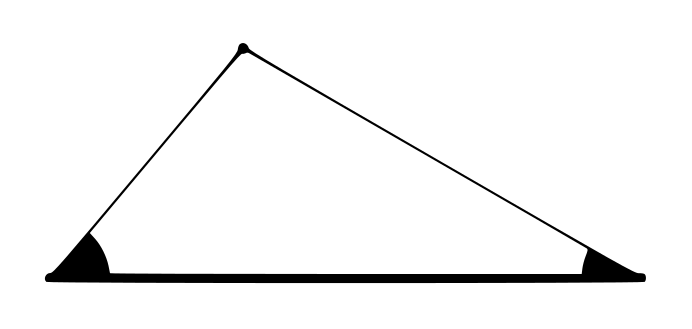
\includegraphics[width=0.35\textwidth,height=\textheight]{figures/fig7.pdf}
\end{center}
& \\
& & \\
Deux côtés et l'angle entre eux & \begin{center}
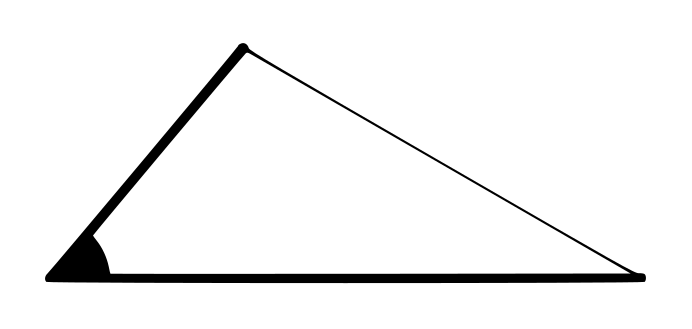
\includegraphics[width=0.35\textwidth,height=\textheight]{figures/fig8.pdf}
\end{center}
& \\
& & \\
Trois côtés & \begin{center}
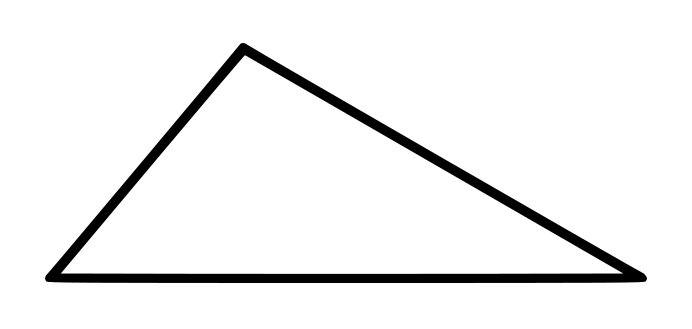
\includegraphics[width=0.35\textwidth,height=\textheight]{figures/fig9.pdf}
\end{center}
& \\
& & \\
Deux côtés et l'angle adjacent à l'un d'eux & \begin{center}
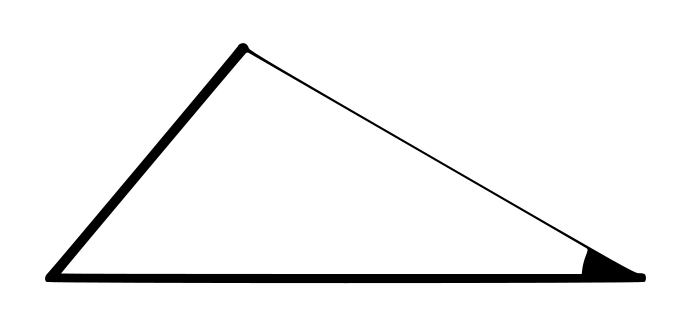
\includegraphics[width=0.35\textwidth,height=\textheight]{figures/fig10.pdf}
\end{center}
& \\
\end{longtable}

\end{exercise}

\newpage

\section{Calculs de distances}\label{calculs-de-distances}

\begin{exercise}[]\protect\hypertarget{exr-}{}\label{exr-}

Dans une nouvelle station de ski, on a installé un téléphérique. Le
câble fait un angle de \(35,4^\circ\) avec le sol supposé horizontal et
il est arrimé à 2 km du pied de la montagne. Quelle est la longueur du
câble, calculée au cm près, si l'on sait que la montagne forme avec le
sol un angle de \(60^\circ\) ?

\begin{center}
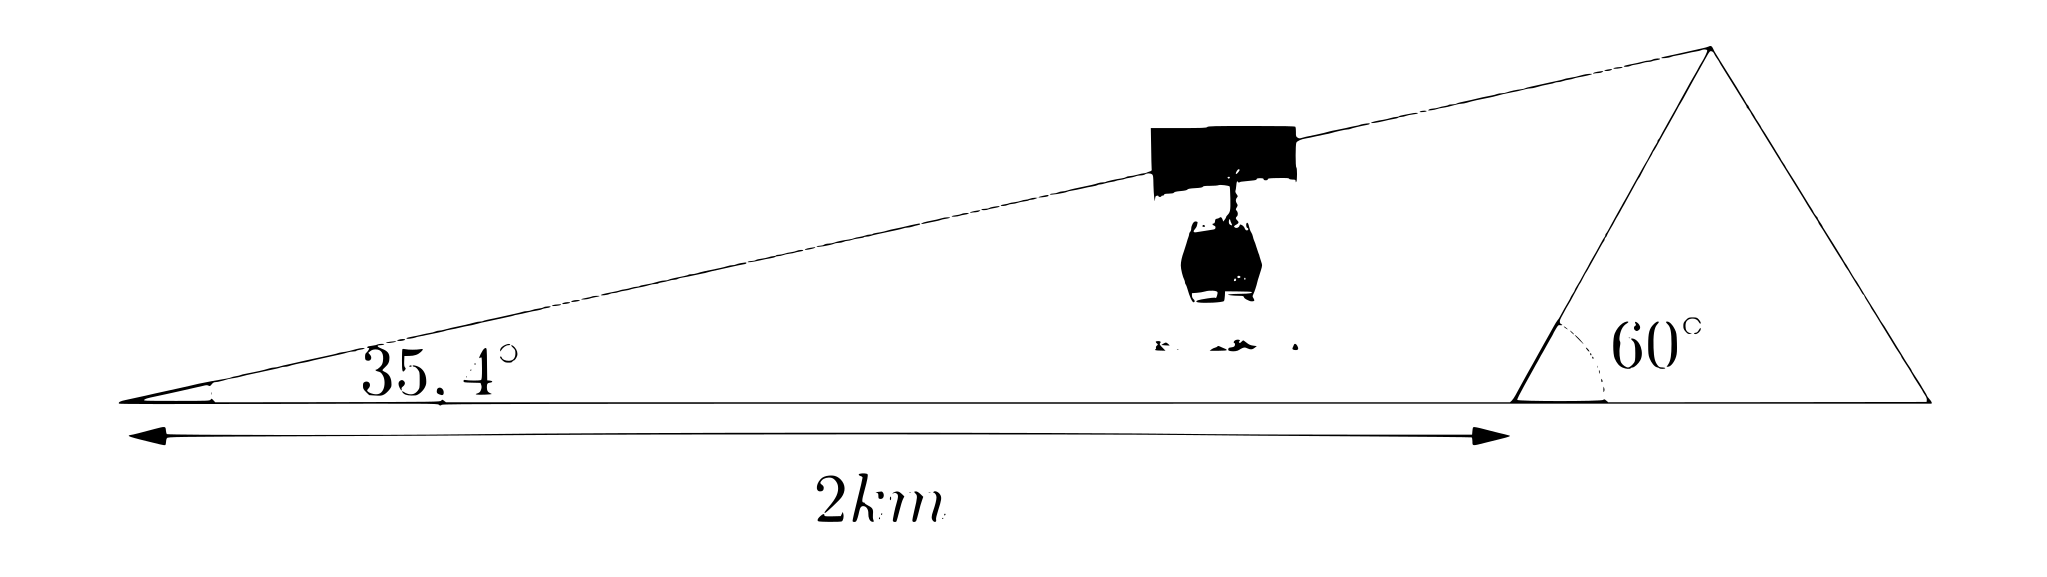
\includegraphics[width=0.65\textwidth,height=\textheight]{figures/fig11.pdf}
\end{center}

\end{exercise}

\begin{exercise}[]\protect\hypertarget{exr-}{}\label{exr-}

L'angle de la pente d'une rue est égal à \(12^\circ\). Sachant que le
soleil se trouve à \(68^\circ\) au-dessus de l'horizontale, calcule la
longueur de l'ombre d'un poteau de 2,5 m de hauteur.

\begin{center}
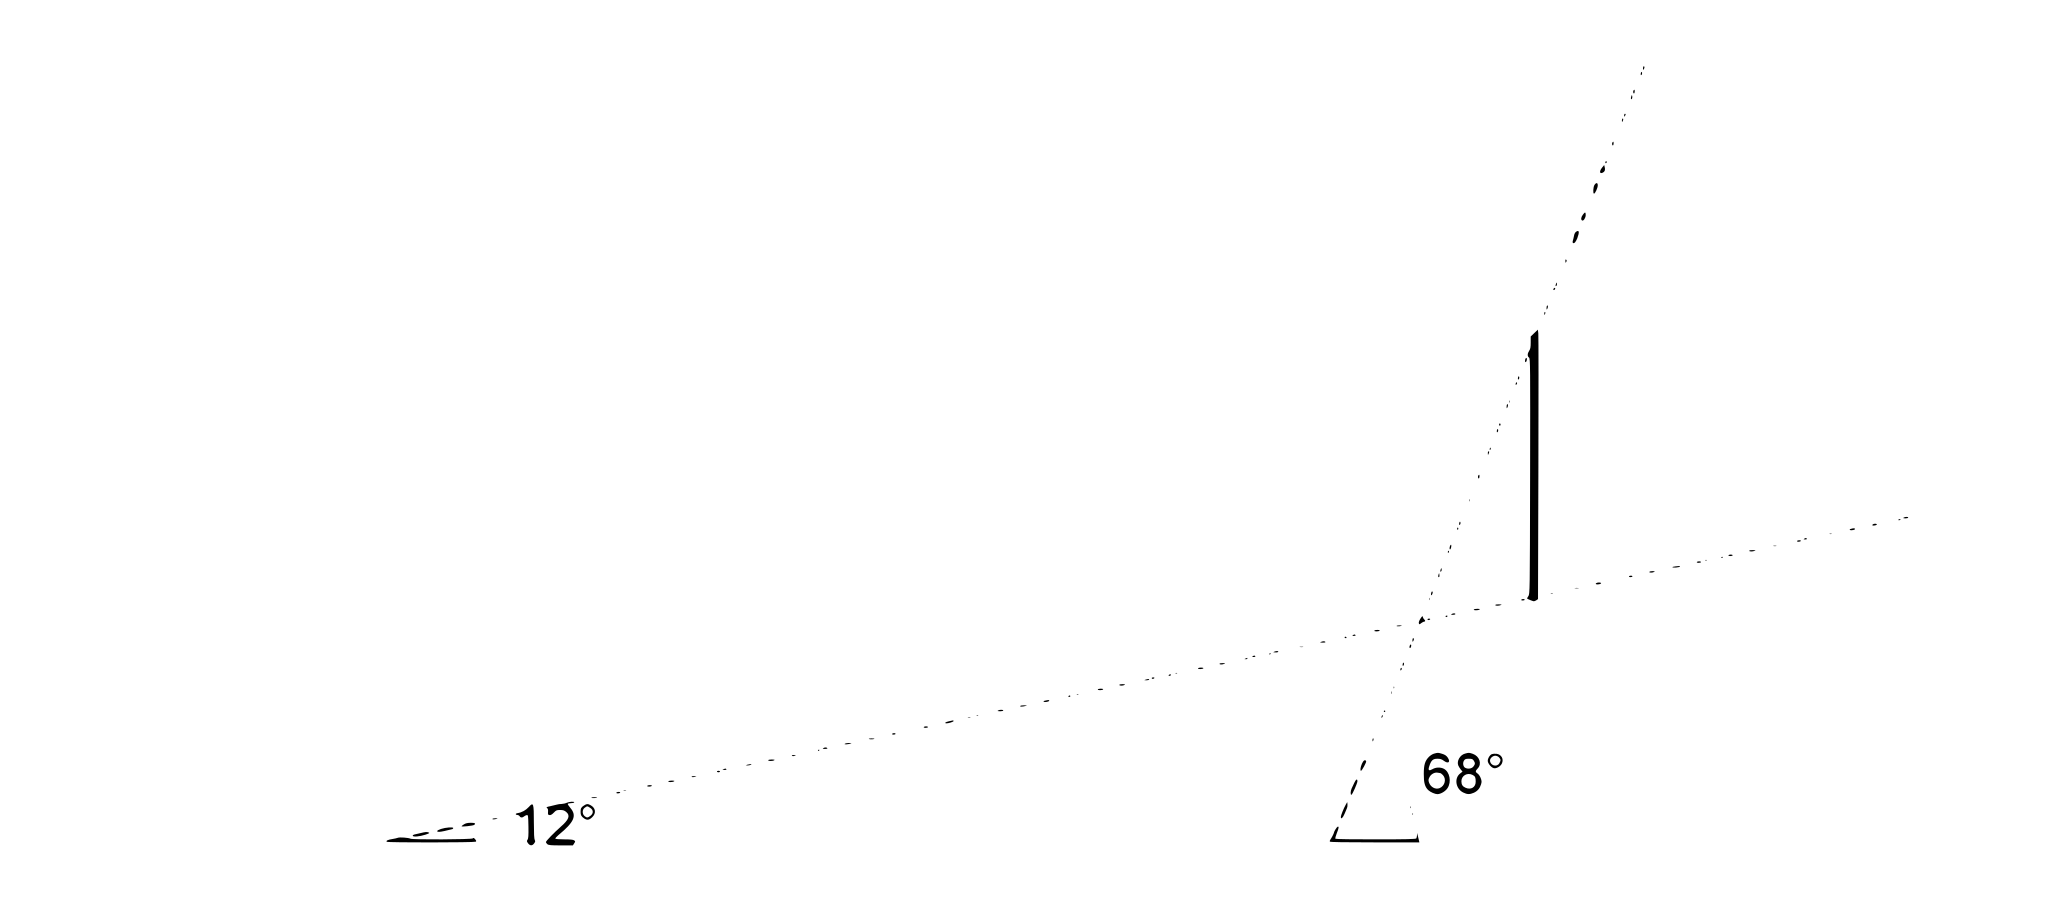
\includegraphics[width=0.65\textwidth,height=\textheight]{figures/fig12.pdf}
\end{center}

\end{exercise}

\begin{exercise}[]\protect\hypertarget{exr-}{}\label{exr-}

Une échelle est appuyée contre un mur vertical construit sur un sol en
pente faisant un angle de \(10^\circ\) par rapport à l'horizontale.
L'échelle fait un angle de 60° par rapport au sol. La distance entre le
bas de l'échelle et le bas du mur est de 2 m (mesurés le long du sol).
Quelle est la longueur de l'échelle et quel angle fait-elle par rapport
au mur ?

\begin{center}
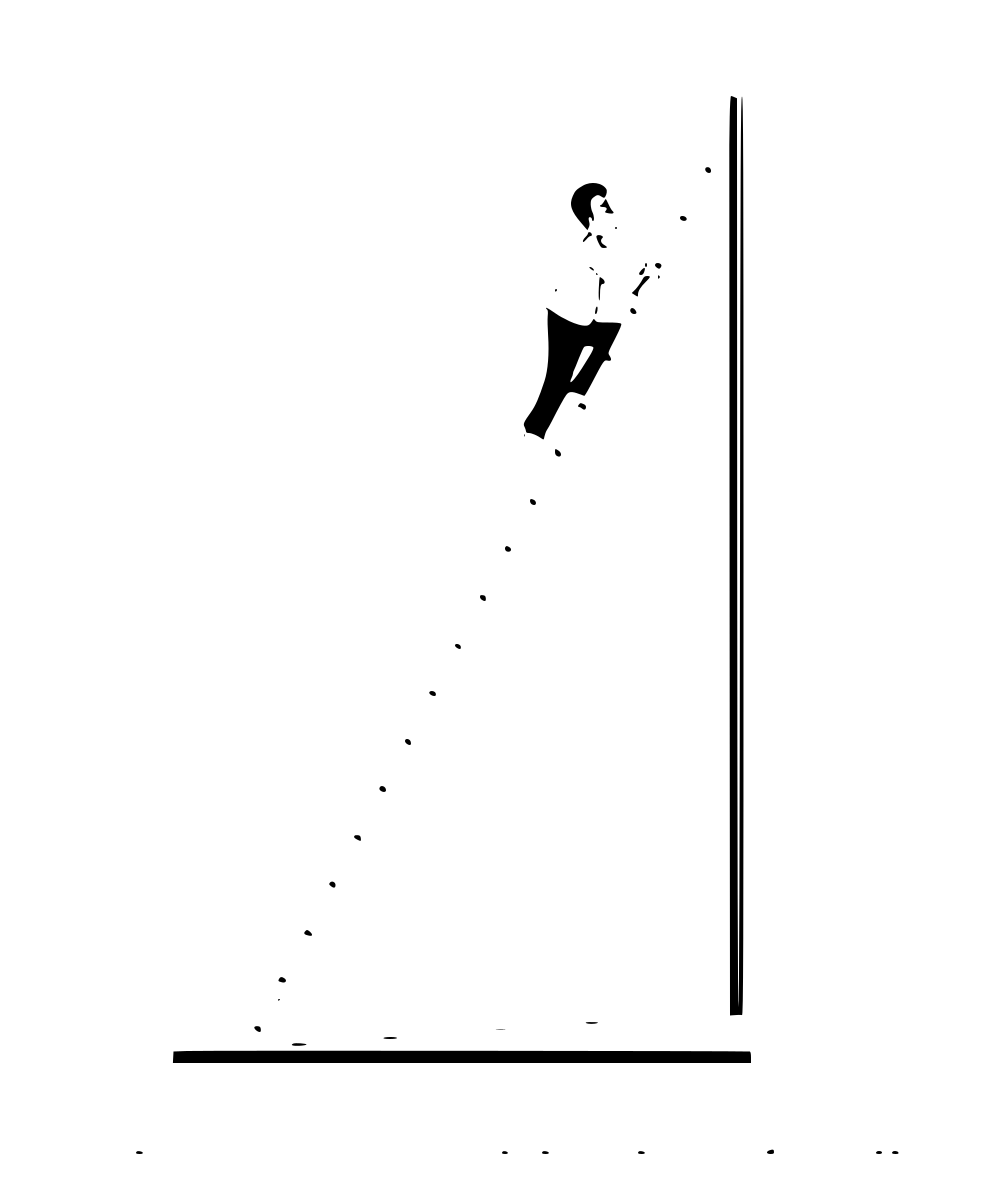
\includegraphics[width=0.4\textwidth,height=\textheight]{figures/fig13.pdf}
\end{center}

\end{exercise}

\begin{exercise}[]\protect\hypertarget{exr-}{}\label{exr-}

Ce schéma représente le parking d'un supermarché. Calcule son aire.

\begin{center}
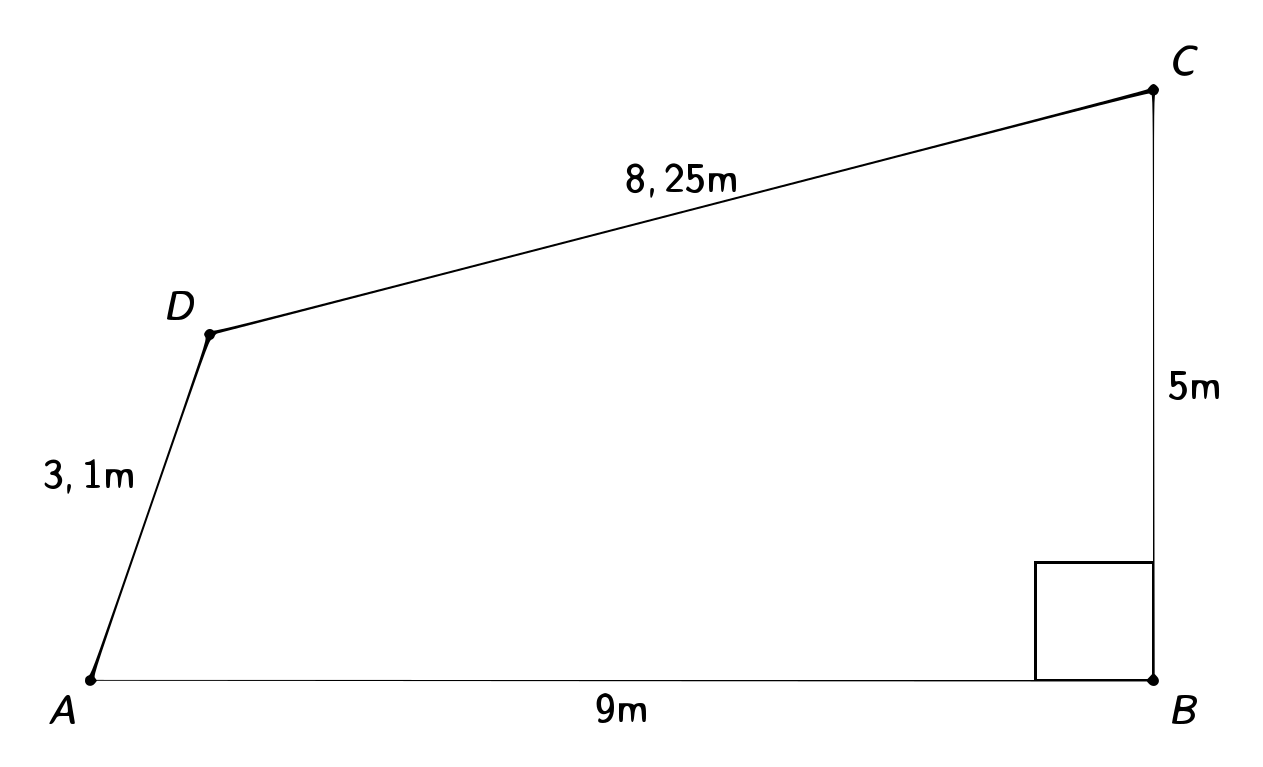
\includegraphics[width=0.4\textwidth,height=\textheight]{figures/fig16.pdf}
\end{center}

\end{exercise}

\begin{exercise}[]\protect\hypertarget{exr-}{}\label{exr-}

Un géomètre désire mesurer la distance horizontale entre deux arbres A
et B séparés par une rivière se trouvant en plaine. Le géomètre choisit
de se placer en un troisième point C (situé sur la même berge que A)
d'où il peut observer les deux arbres. A partir de ce point, il voit les
deux arbres sous un angle de \(154^\circ\). Il se place ensuite en A et
voit les points B et C sous un angle de \(17^\circ\). La distance
séparant les points A et C vaut 28 m. Quelle est la distance entre les
deux arbres ?

\begin{center}
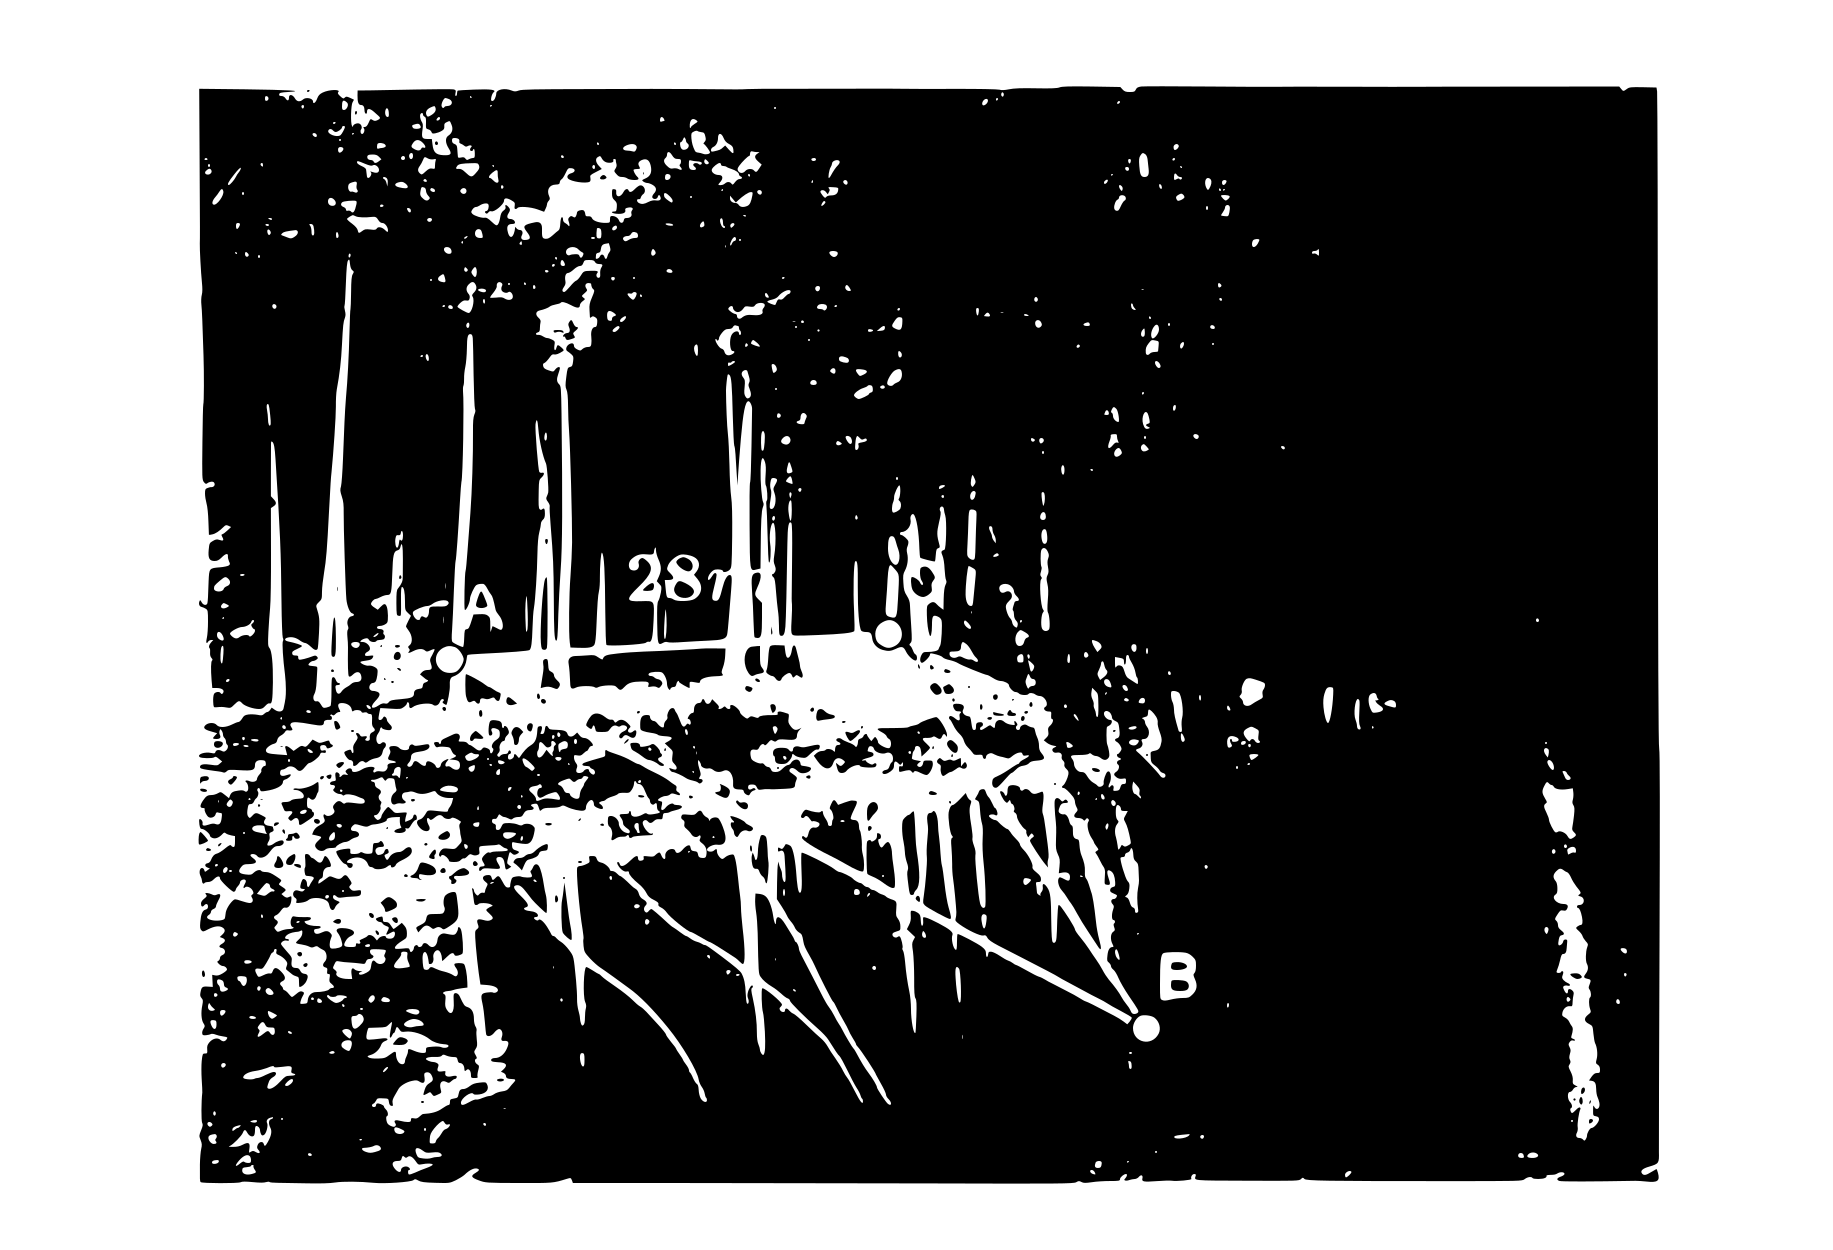
\includegraphics[width=0.65\textwidth,height=\textheight]{figures/fig15.pdf}
\end{center}

\end{exercise}

\bookmarksetup{startatroot}

\chapter{Trigonométrie des angles
obtus}\label{trigonomuxe9trie-des-angles-obtus}

\section{Introduction: rotations et nombres
trigonométriques}\label{introduction-rotations-et-nombres-trigonomuxe9triques}

Sur le repère ci-dessous,

\begin{enumerate}
\def\labelenumi{\arabic{enumi})}
\item
  place les points \(O=(0;0)\), \(I=(1;0)\) et \(J=(0;1)\).
\item
  dessine ensuite le point \(P_1\), image du point \(I\) par une
  rotation de centre \(O\) et d'angle \(+30^\circ\).
\item
  Fais de même pour les points \(P_2\) et \(P_3\), images de \(I\) par
  les rotations de centre \(O\) et d'angles respectifs \(+45^\circ\) et
  \(+60^\circ\).
\item
  Complète le tableau suivant:
\end{enumerate}

\begin{longtable}[]{@{}
  >{\raggedright\arraybackslash}p{(\columnwidth - 10\tabcolsep) * \real{0.1398}}
  >{\raggedright\arraybackslash}p{(\columnwidth - 10\tabcolsep) * \real{0.1613}}
  >{\raggedright\arraybackslash}p{(\columnwidth - 10\tabcolsep) * \real{0.1290}}
  >{\raggedright\arraybackslash}p{(\columnwidth - 10\tabcolsep) * \real{0.1183}}
  >{\raggedright\arraybackslash}p{(\columnwidth - 10\tabcolsep) * \real{0.2043}}
  >{\raggedright\arraybackslash}p{(\columnwidth - 10\tabcolsep) * \real{0.2043}}@{}}
\toprule\noalign{}
\multirow{2}{=}{\begin{minipage}[b]{\linewidth}\raggedright
Angle
\end{minipage}} &
\multirow{2}{=}{\begin{minipage}[b]{\linewidth}\raggedright
Image de \(I\)
\end{minipage}} &
\multicolumn{2}{>{\raggedright\arraybackslash}p{(\columnwidth - 10\tabcolsep) * \real{0.2473} + 2\tabcolsep}}{%
\begin{minipage}[b]{\linewidth}\raggedright
Coordonnées du point
\end{minipage}} &
\multicolumn{2}{>{\raggedright\arraybackslash}p{(\columnwidth - 10\tabcolsep) * \real{0.4086} + 2\tabcolsep}@{}}{%
\begin{minipage}[b]{\linewidth}\raggedright
Nombres trigonométriques de l'angle
\end{minipage}} \\
& & \begin{minipage}[b]{\linewidth}\raggedright
abscisse
\end{minipage} & \begin{minipage}[b]{\linewidth}\raggedright
ordonnée
\end{minipage} & \begin{minipage}[b]{\linewidth}\raggedright
\(\cos\)
\end{minipage} & \begin{minipage}[b]{\linewidth}\raggedright
\(\sin\)
\end{minipage} \\
\midrule\noalign{}
\endhead
\bottomrule\noalign{}
\endlastfoot
\(30^\circ\) & & & & & \\
\(45^\circ\) & & & & & \\
\(60^\circ\) & & & & & \\
& \(J\) & & & & \\
\end{longtable}

\begin{center}
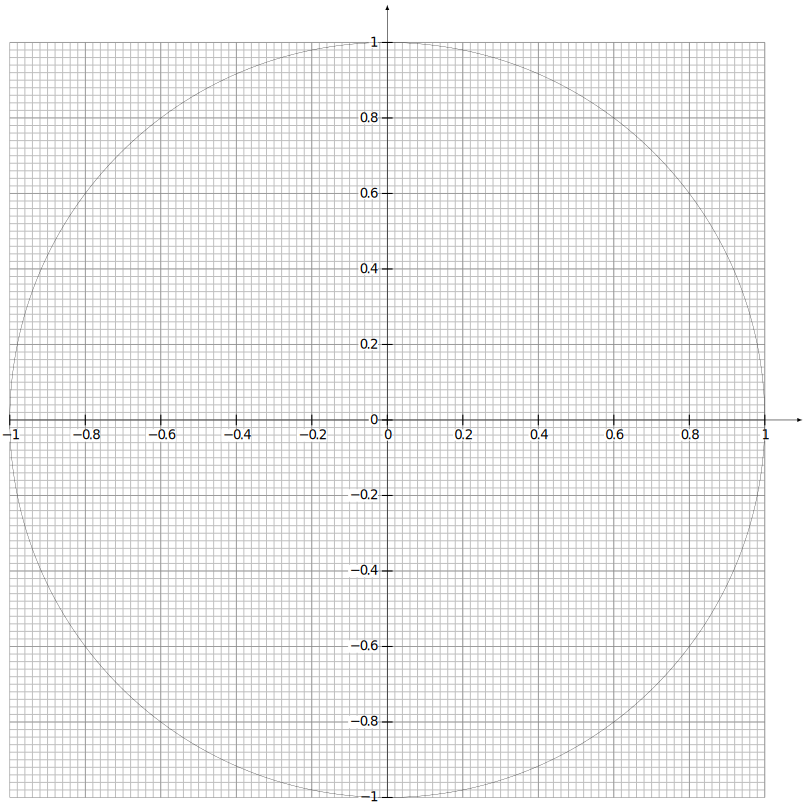
\includegraphics[width=0.55\textwidth,height=\textheight]{figures/CT.pdf}
\end{center}

On observe, grâce au tableau, que l'image \(P\) de \(I\) par une
rotation de centre \(O\) et d'angle \(\alpha\) (compris en 0 et 90
degrés) a pour coordonnées:
\(P=(\makebox[2cm]{\dotfill};\makebox[2cm]{\dotfill})\).

\begin{exercise}[]\protect\hypertarget{exr-rot}{}\label{exr-rot}

~

\begin{enumerate}
\def\labelenumi{\arabic{enumi})}
\item
  Dessine, dans le repère ci-dessous, les points \(P_4\), \(P_5\),
  \(P_6\), \ldots, images du point \(I\) par rotation de centre \(O\) et
  d'angles \(-30^\circ\), \(-45^\circ\), \(120^\circ\), \(135^\circ\),
  \(180^\circ\), \(210^\circ\), \(270^\circ\), \(360^\circ\).
\item
  En te basant sur l'observation faite à partir du tableau de la page
  précédente, complète le tableau suivant.
\end{enumerate}

\begin{longtable}[]{@{}
  >{\raggedright\arraybackslash}p{(\columnwidth - 6\tabcolsep) * \real{0.1944}}
  >{\raggedright\arraybackslash}p{(\columnwidth - 6\tabcolsep) * \real{0.2083}}
  >{\raggedright\arraybackslash}p{(\columnwidth - 6\tabcolsep) * \real{0.1667}}
  >{\raggedright\arraybackslash}p{(\columnwidth - 6\tabcolsep) * \real{0.1528}}@{}}
\toprule\noalign{}
\multirow{2}{=}{\begin{minipage}[b]{\linewidth}\raggedright
Angle
\end{minipage}} &
\multirow{2}{=}{\begin{minipage}[b]{\linewidth}\raggedright
Image de \(I\)
\end{minipage}} &
\multicolumn{2}{>{\raggedright\arraybackslash}p{(\columnwidth - 6\tabcolsep) * \real{0.3194} + 2\tabcolsep}@{}}{%
\begin{minipage}[b]{\linewidth}\raggedright
Coordonnées du point
\end{minipage}} \\
& & \begin{minipage}[b]{\linewidth}\raggedright
abscisse
\end{minipage} & \begin{minipage}[b]{\linewidth}\raggedright
ordonnée
\end{minipage} \\
\midrule\noalign{}
\endhead
\bottomrule\noalign{}
\endlastfoot
\(-30^\circ\) & & & \\
\(-45^\circ\) & & & \\
\(120^\circ\) & & & \\
\(135^\circ\) & & & \\
\(180^\circ\) & & & \\
\(210^\circ\) & & & \\
\(270^\circ\) & & & \\
\(360^\circ\) & & & \\
\end{longtable}

\end{exercise}

\begin{center}
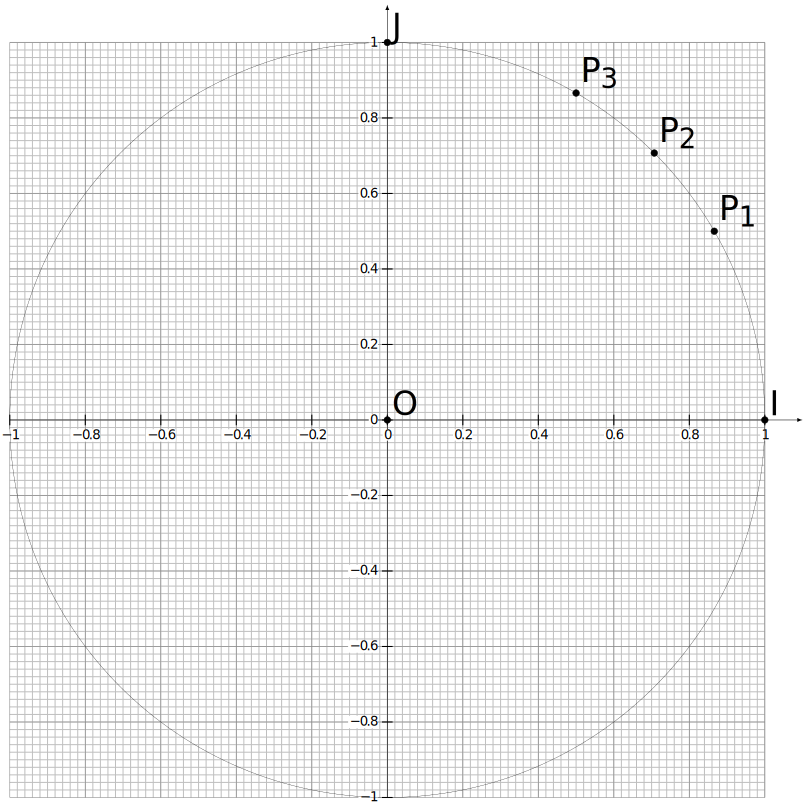
\includegraphics[width=0.75\textwidth,height=\textheight]{figures/CT2.pdf}
\end{center}

\section{Angles orientés}\label{angles-orientuxe9s}

Les angles sont utiles pour discuter des mouvement circulaires. Les
angles permettent de décrire des rotations, le mouvement d'un passager
d'une grande roue, le mouvement de la valve d'un pneu de voiture, etc.

Afin d'être le plus précis possible, il est utile d'utiliser la notion
d'angle orienté. Cette notion permettra de distinguer, concernant la
valve d'un pneu d'une voiture, lorsqu'elle tourne en allant de l'avant
ou lorsqu'elle toune en allant en arrière.

\begin{definition}[]\protect\hypertarget{def-angles}{}\label{def-angles}

Un \emph{angle} \(\alpha\) est donné à l'aide de deux rayons
\(\overline{OA}\) et \(\overline{OB}\). Cet angle peut représenter deux
rotations: une qui va de \(A\) vers \(B\) et l'autre de \(B\) vers
\(A\).

\begin{center}
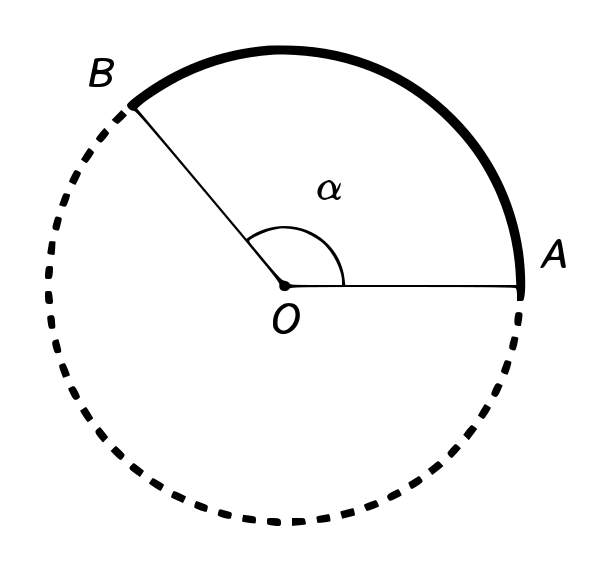
\includegraphics[width=0.3\textwidth,height=\textheight]{figures/fig17.pdf}
\end{center}

Un \emph{angle orienté} sera donné par deux rayons \(\overline{OA}\) et
\(\overline{OB}\). L'un des rayons sera l'origine et l'autre
l'extrémité, ce qui permettra de préciser le sens de la rotation. Si la
rotation se fait dans le sens contraire des aiguilles d'une montre
(\emph{dans le sens trigonométrique}), alors \(\alpha\ge0\). Dans le cas
contraire, \(\alpha<0\).

\begin{center}
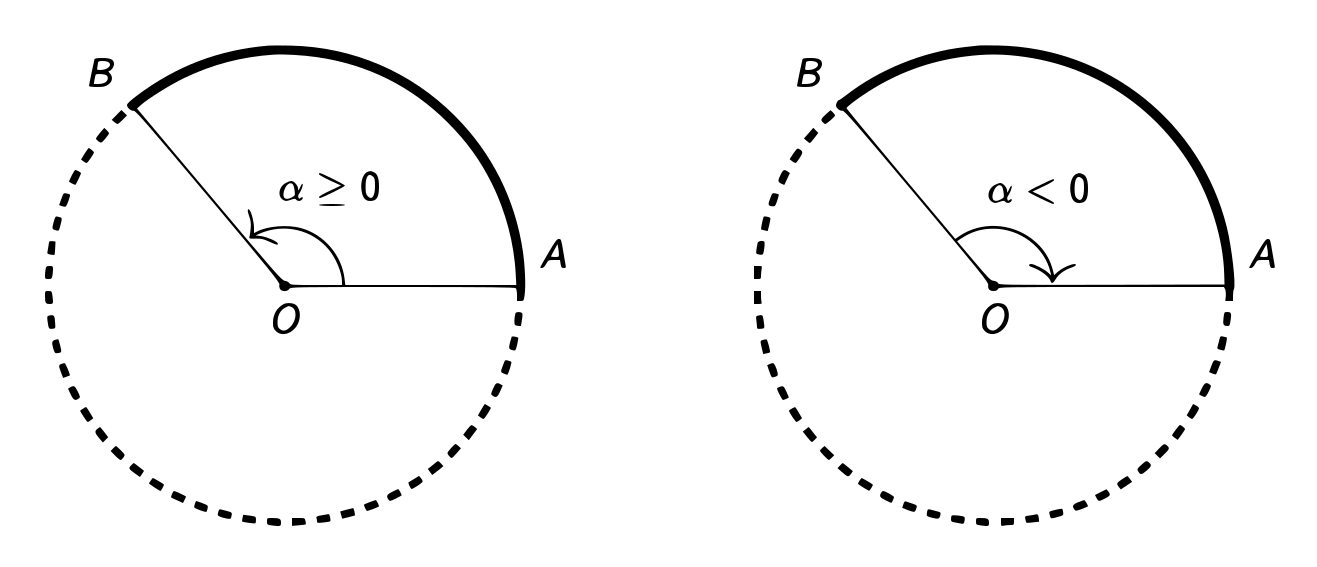
\includegraphics[width=0.6\textwidth,height=\textheight]{figures/fig18.pdf}
\end{center}

\end{definition}

\section{Le cercle trigonométrique}\label{le-cercle-trigonomuxe9trique}

\begin{definition}[]\protect\hypertarget{def-ct}{}\label{def-ct}

Le cercle trigonométrique est un cercle de rayon 1 centré à l'origine
d'un repère. Ce cercle sera utilisé pour représenter les angles
orientés, en prenant toujours comme origine le point (1;0). De plus, ce
cercle sera utilisé plus tard pour définir les nombres trigonométriques
(\(\sin\), \(\cos\) et \(\tan\)). Pour représenter les tangentes, on
ajoutera un axe vertical passant par \((0;1)\).

\begin{center}
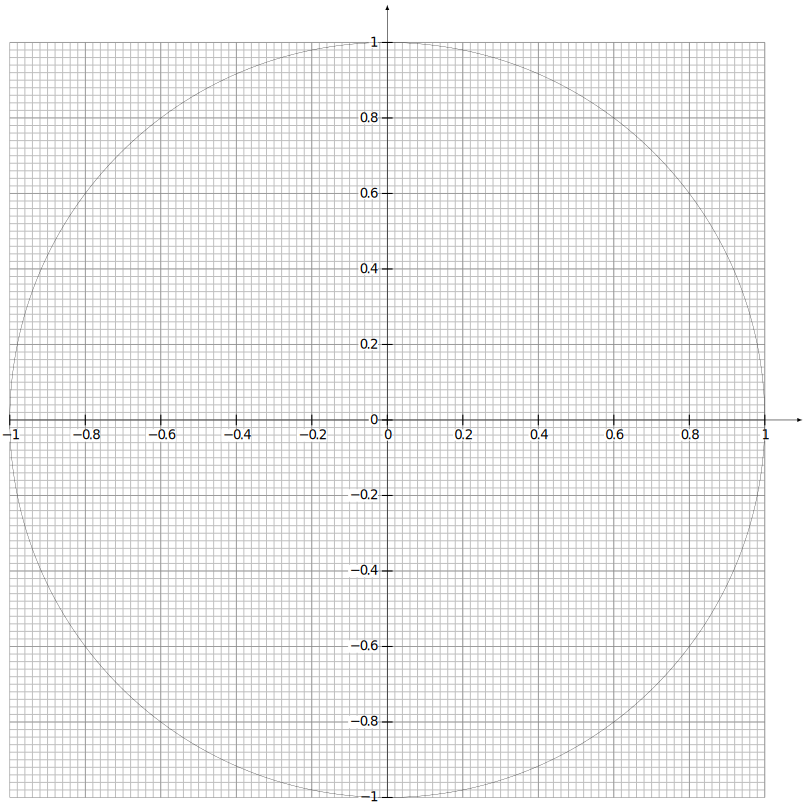
\includegraphics[width=0.4\textwidth,height=\textheight]{figures/CT.pdf}
\end{center}

\end{definition}

Le cercle trigonométrique est découpé en quatre parties appelées
\emph{quadrants}.

\begin{center}
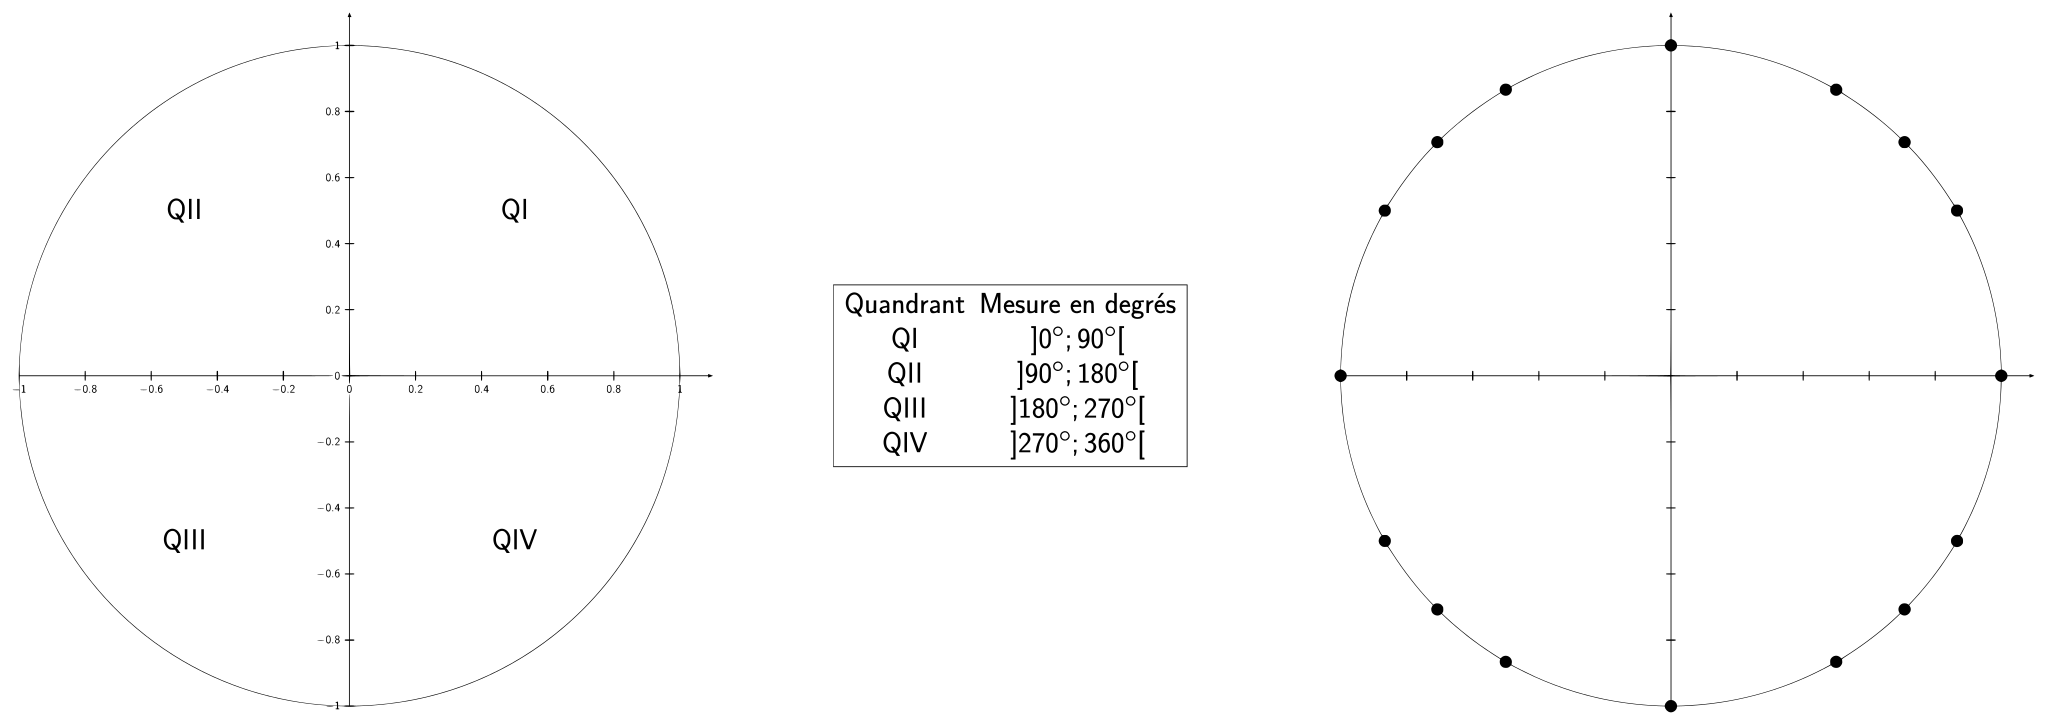
\includegraphics[width=1\textwidth,height=\textheight]{figures/fig19.pdf}
\end{center}

\section{Sinus et cosinus dans le cercle
trigonométrique}\label{sinus-et-cosinus-dans-le-cercle-trigonomuxe9trique}

\subsection{Définition}\label{duxe9finition}

\begin{definition}[]\protect\hypertarget{def-sincos}{}\label{def-sincos}

Soit \(\alpha\) un angle et \(P\) le point correspondant sur le cercle
trigonométrique. Alors:

\begin{enumerate}
\def\labelenumi{\arabic{enumi}.}
\tightlist
\item
  le \emph{cosinus} de \(\alpha\), noté \(\cos(\alpha)\), est l'abscisse
  du point \(P\)
\item
  le \emph{sinus} de \(\alpha\), noté \(\sin(\alpha)\), est l'ordonnée
  du point \(P\)
\end{enumerate}

\begin{center}
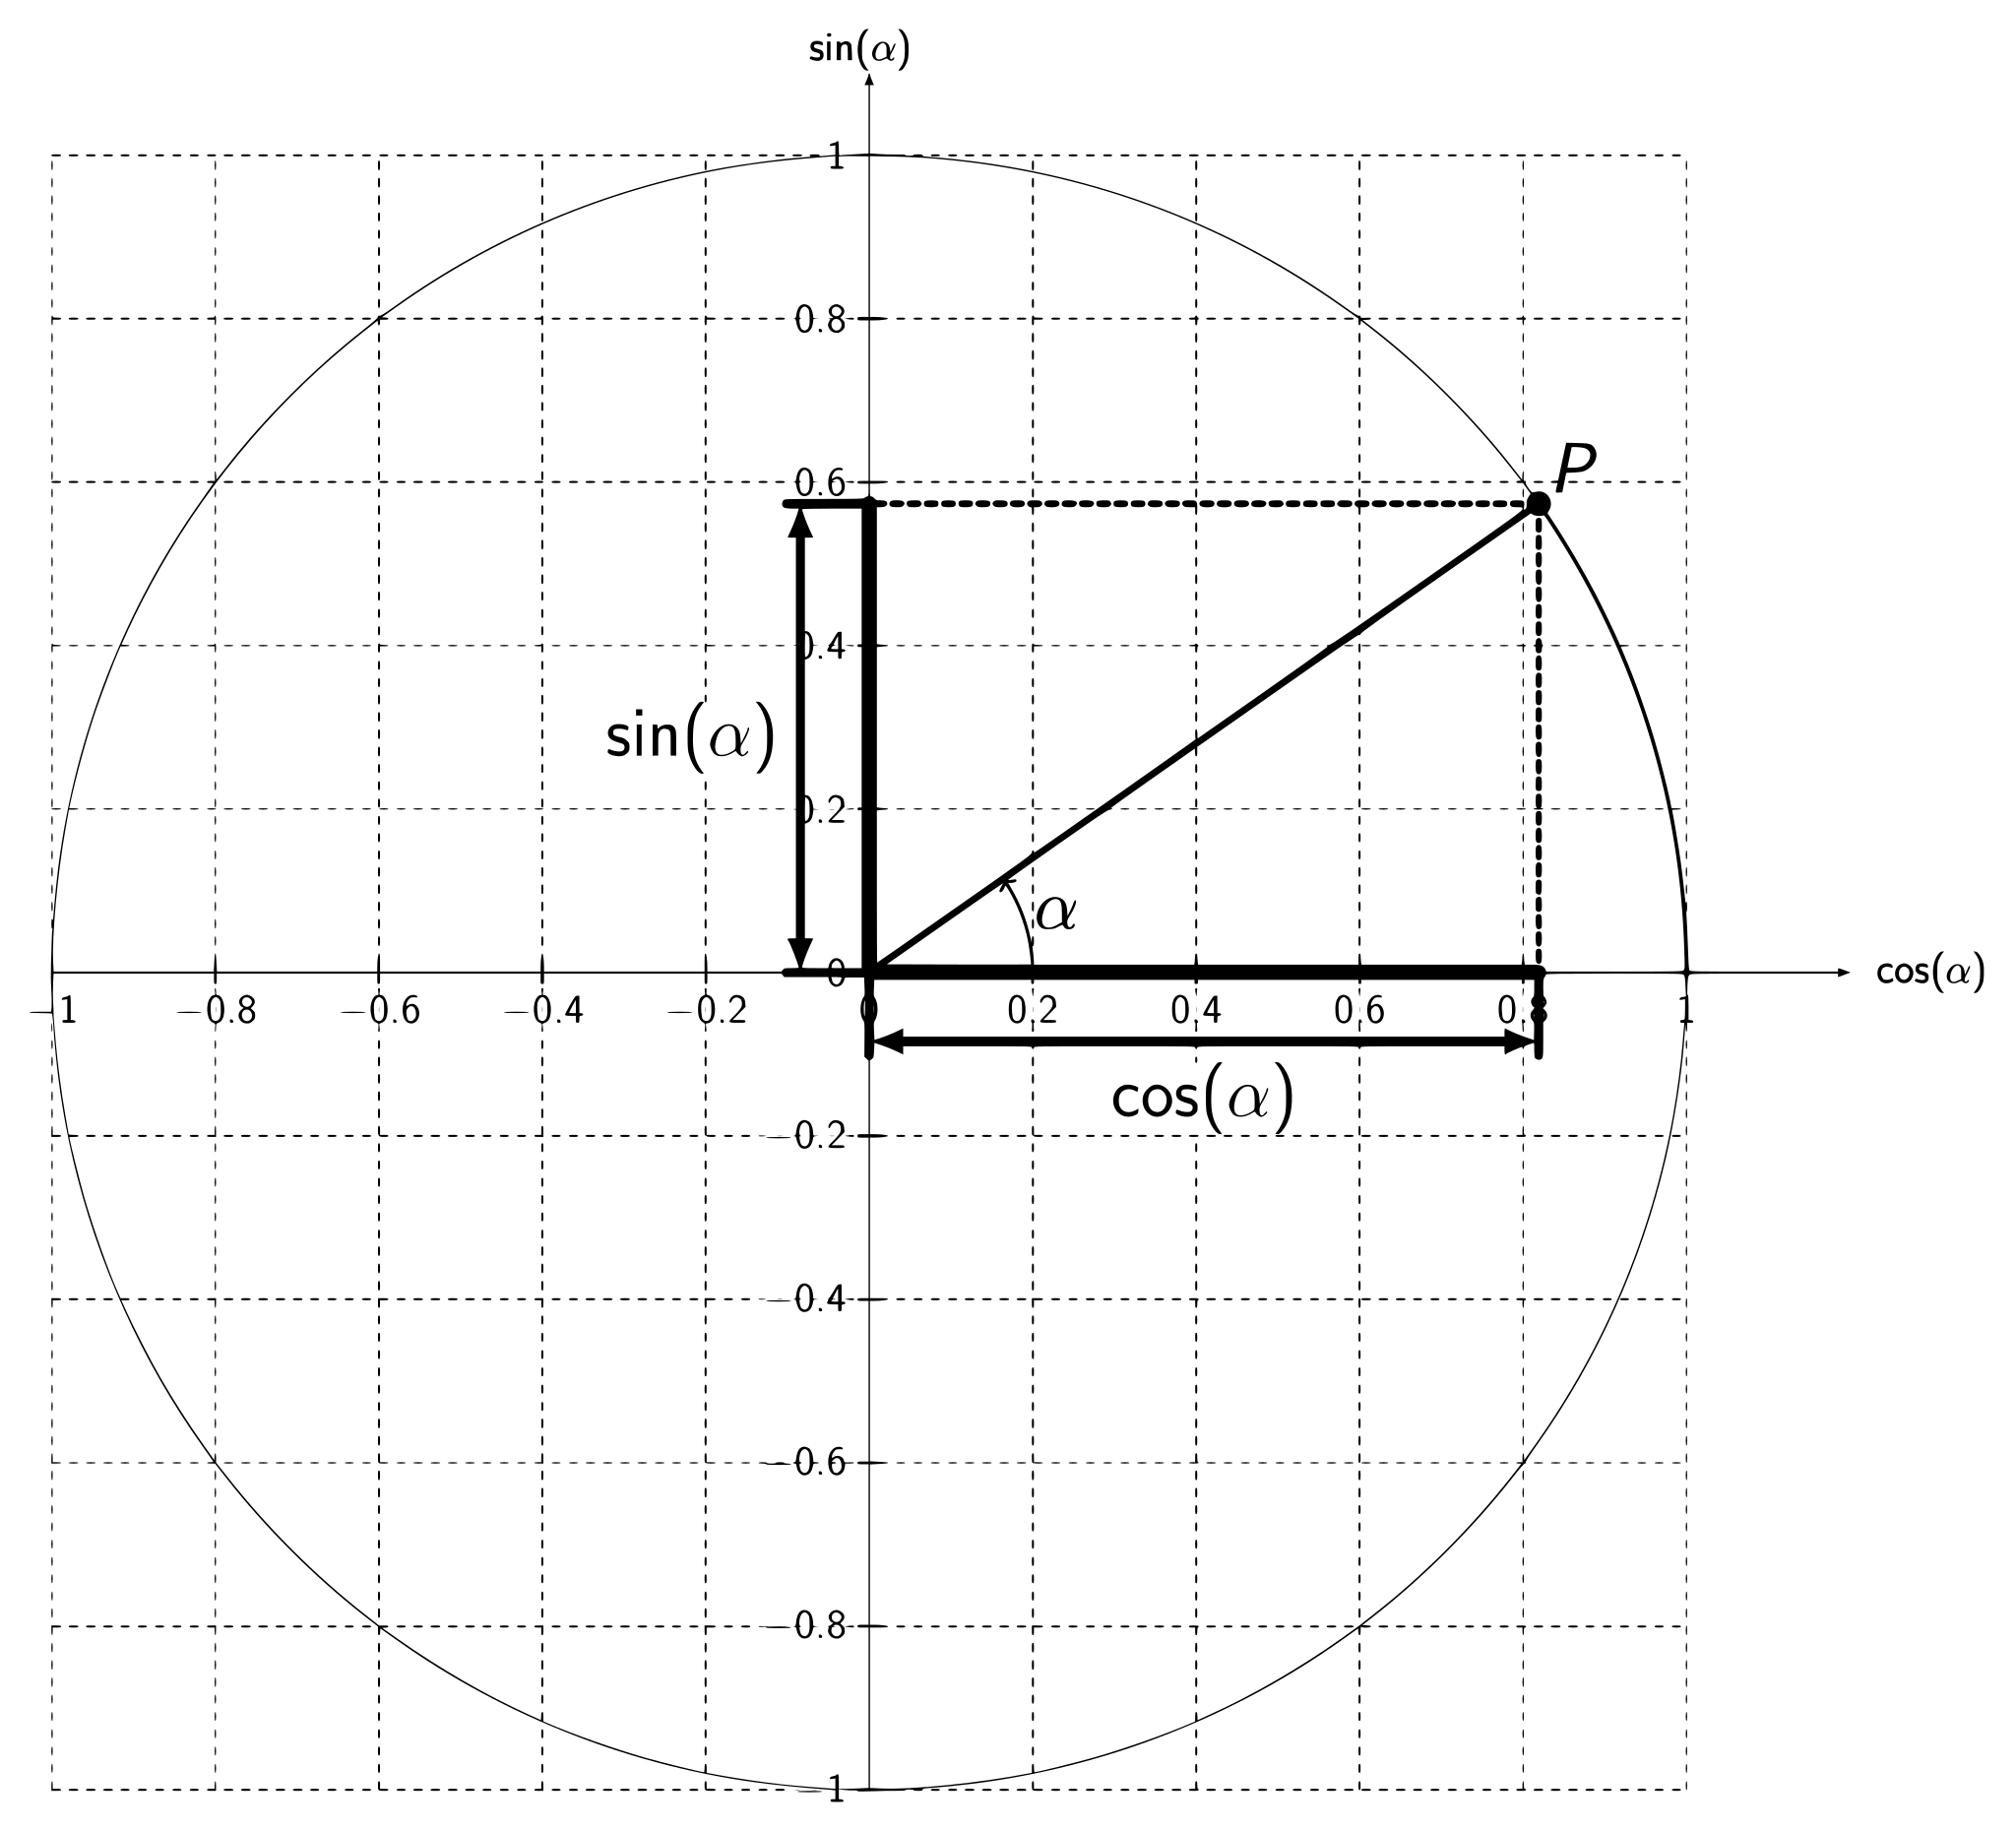
\includegraphics[width=0.5\textwidth,height=\textheight]{figures/fig20.pdf}
\end{center}

\end{definition}

\begin{example}[]\protect\hypertarget{exm-sincos}{}\label{exm-sincos}

~

\begin{figure}

\begin{minipage}{0.60\linewidth}
\begin{center}
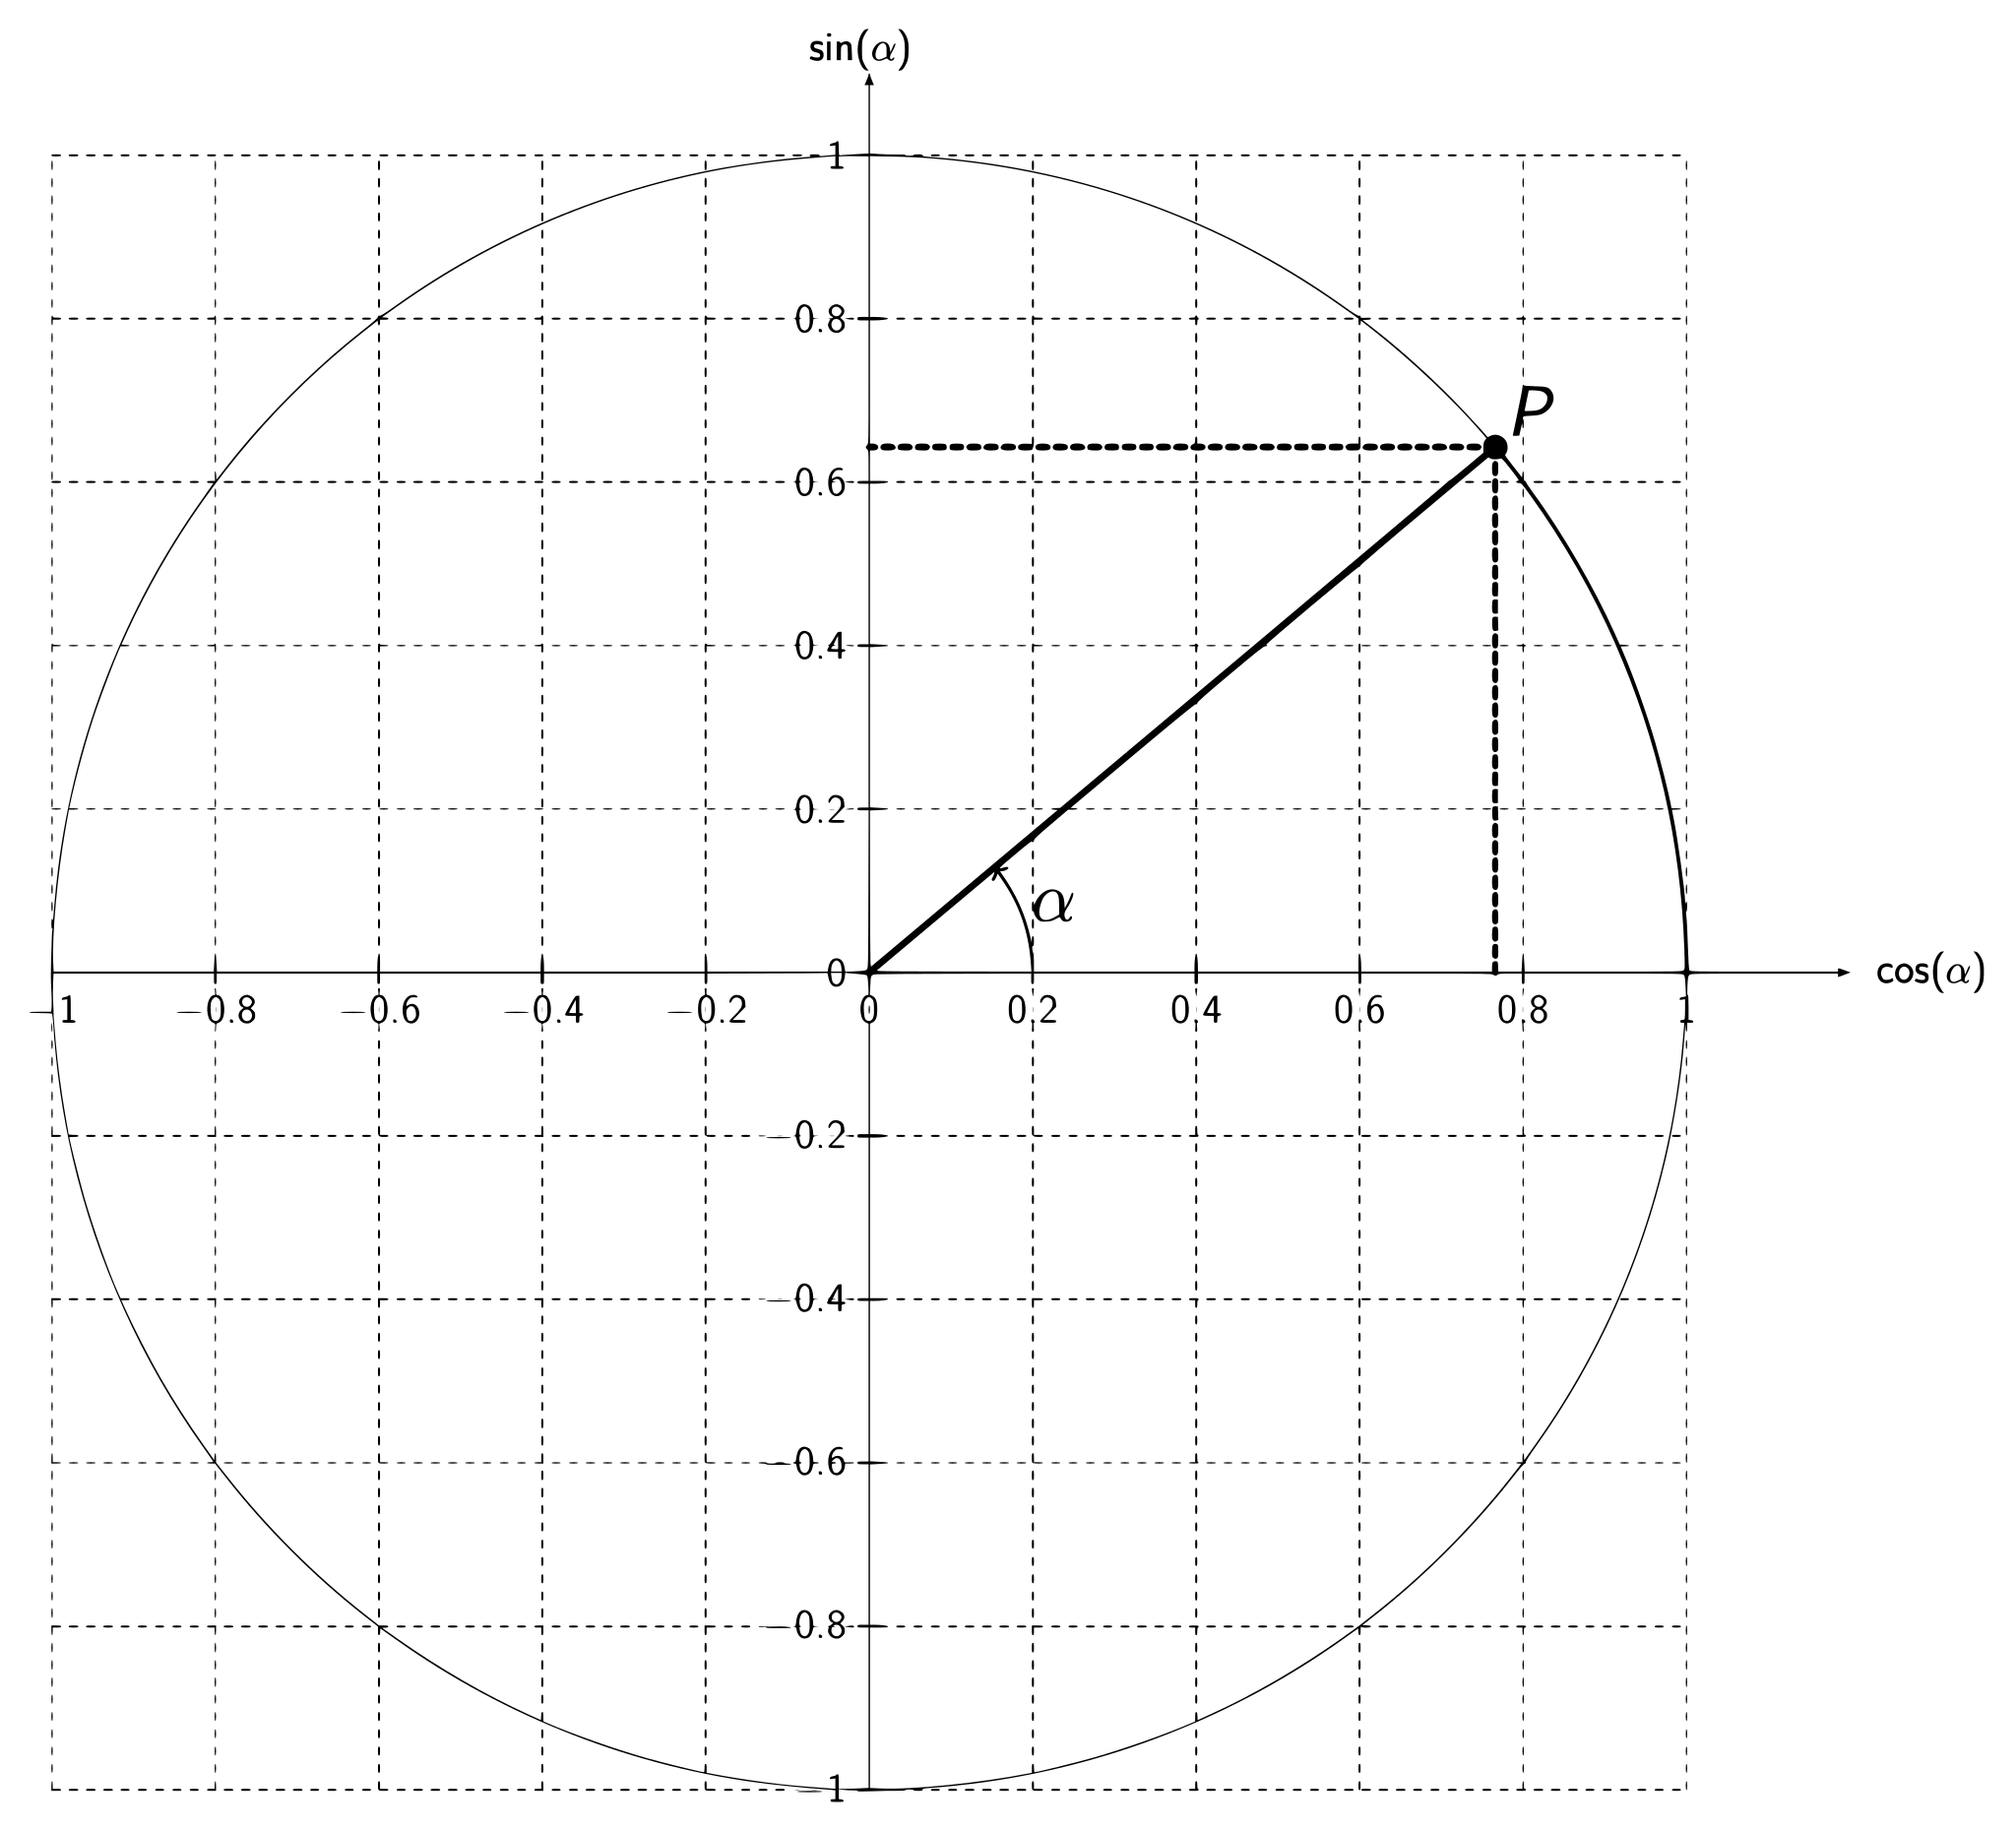
\includegraphics{figures/fig21.pdf}
\end{center}
\end{minipage}%
%
\begin{minipage}{0.40\linewidth}

\begin{enumerate}
\def\labelenumi{\arabic{enumi})}
\item
  Quand le point \(P\) s'approche du point \((1;0)\), l'angle \(\alpha\)
  s'approche de \(0^\circ\). Donc

  \(\cos(0)=\makebox[2cm]{\dotfill}\)

  \(\sin(0)=\makebox[2cm]{\dotfill}\)
\item
  Quand le point \(P\) s'approche du point \((0;1)\), l'angle \(\alpha\)
  s'approche de \(90^\circ\). Donc

  \(\cos(90)=\makebox[2cm]{\dotfill}\)

  \(\sin(90)=\makebox[2cm]{\dotfill}\)
\end{enumerate}

\end{minipage}%

\end{figure}%

\end{example}

\subsection{Représentation dans chaque
quadrant}\label{repruxe9sentation-dans-chaque-quadrant}

\begin{center}
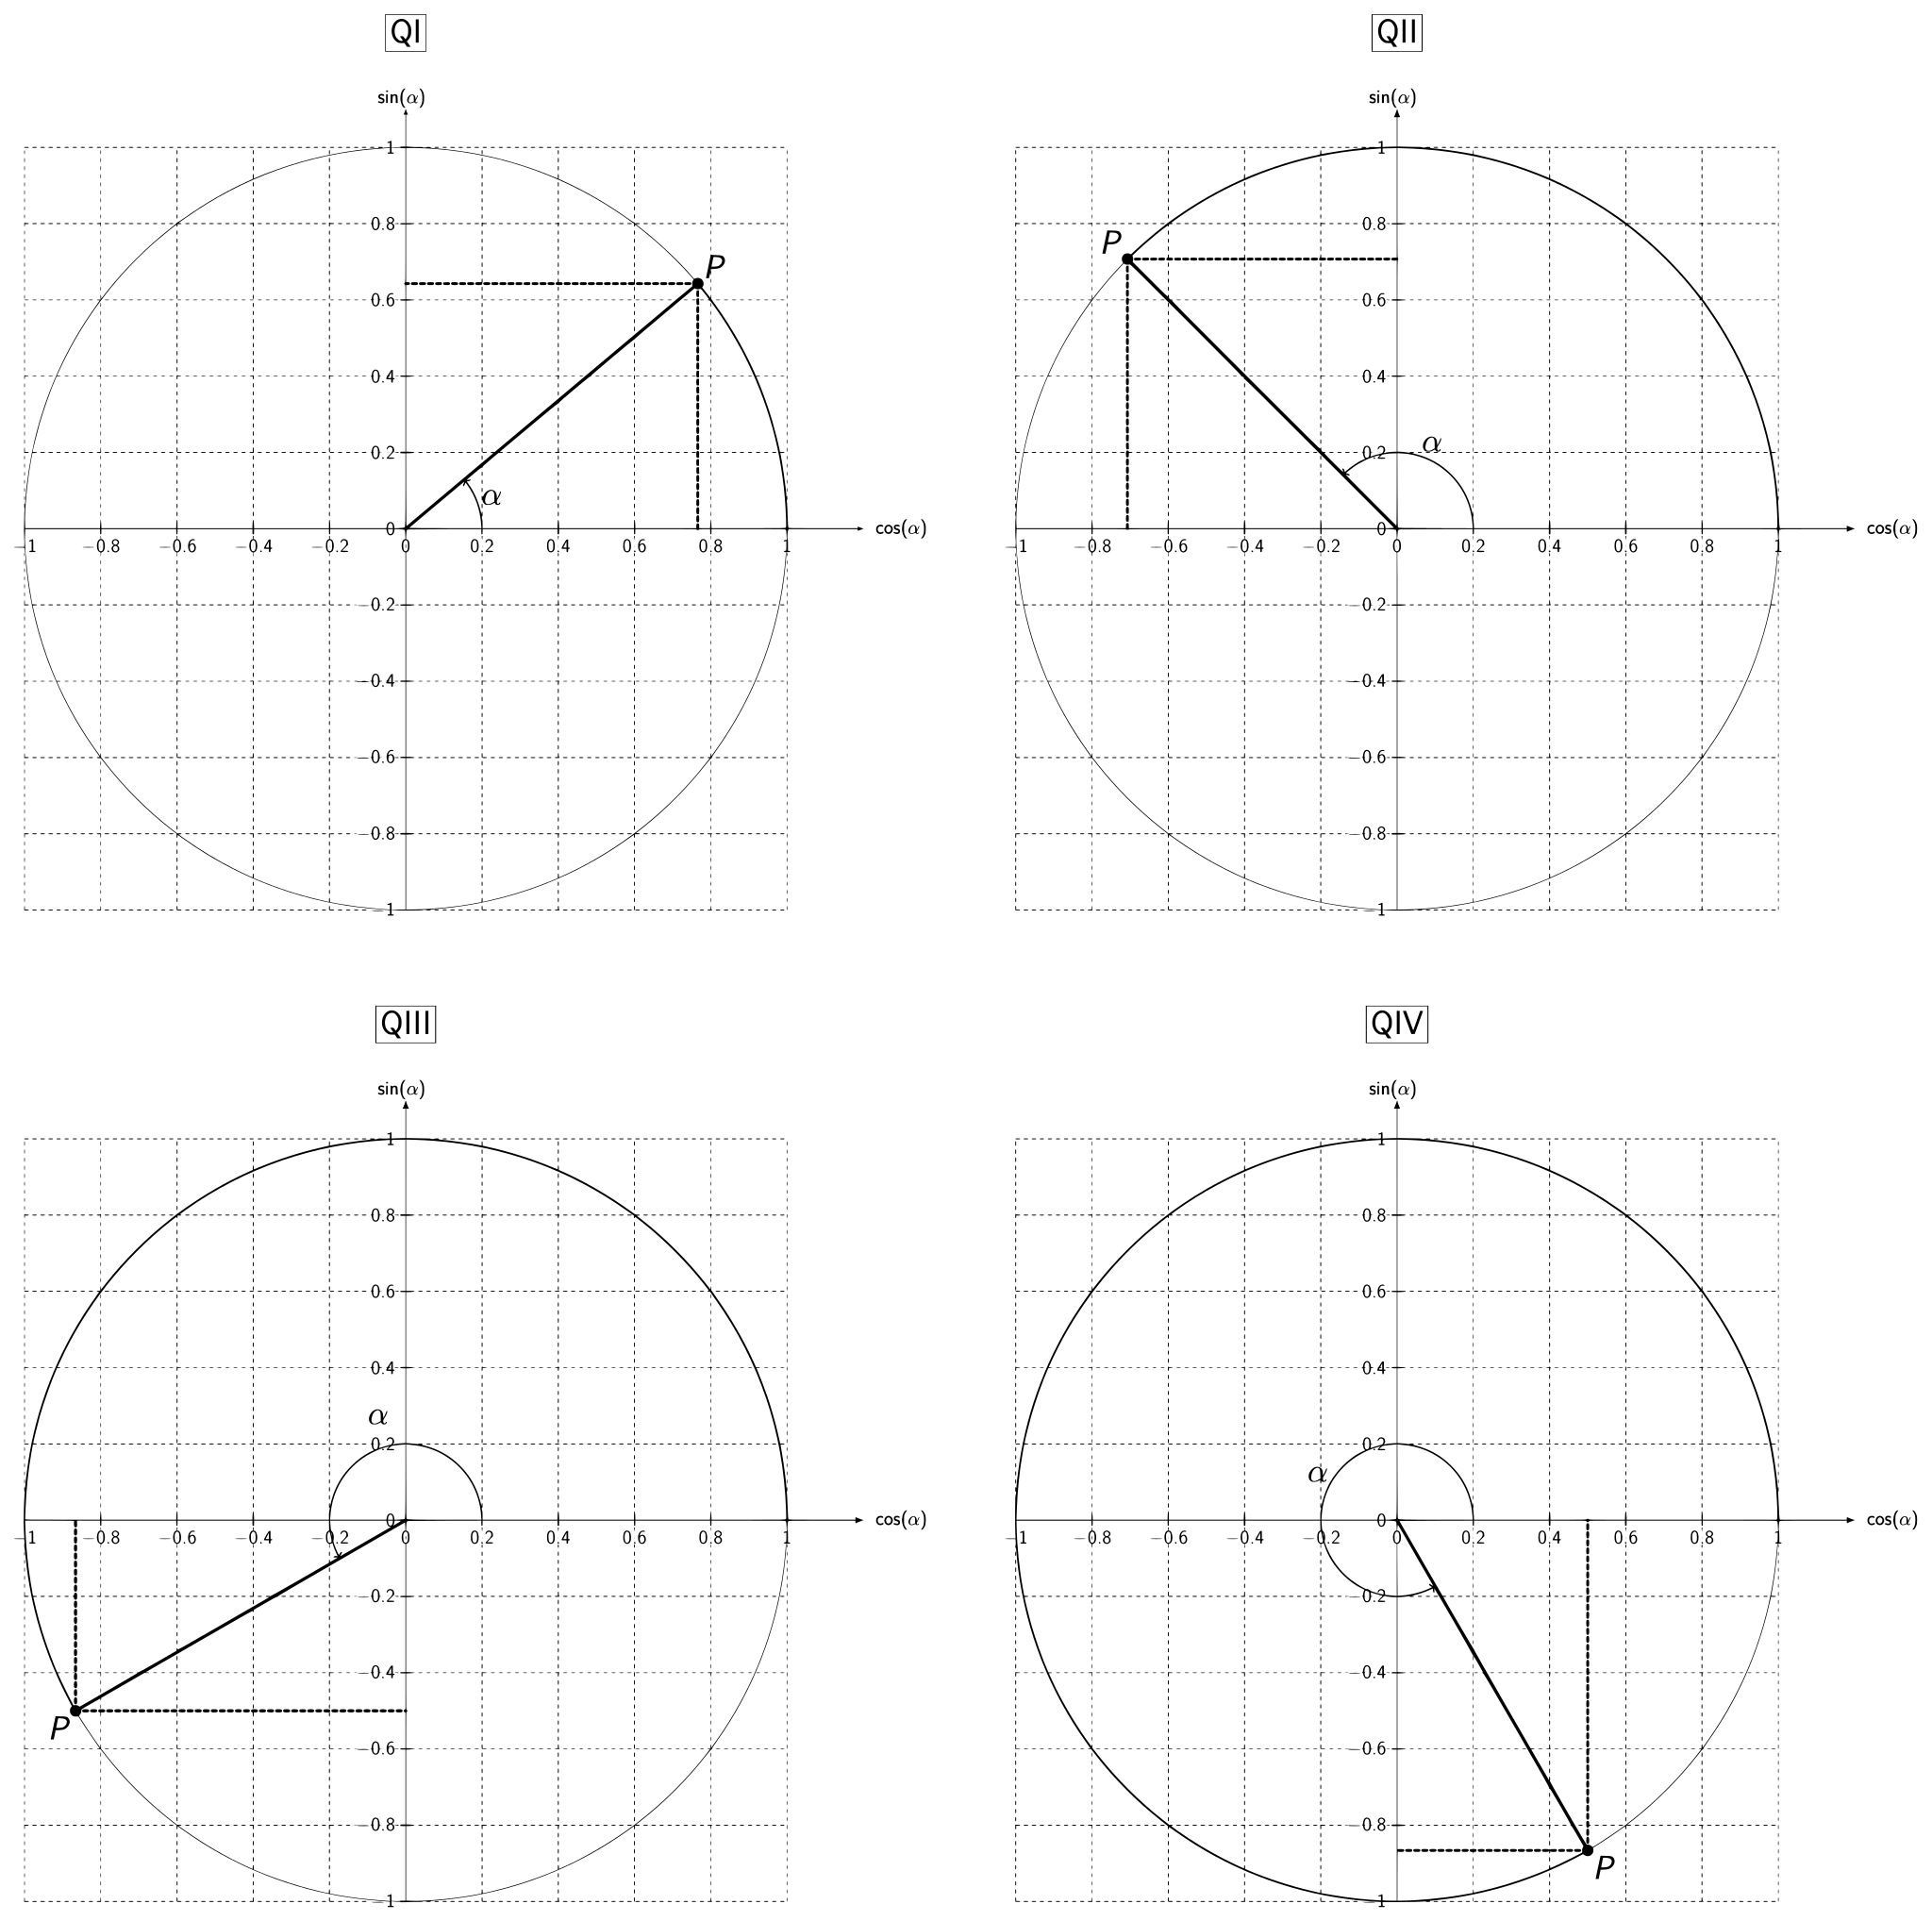
\includegraphics[width=0.8\textwidth,height=\textheight]{figures/fig22.pdf}
\end{center}

\begin{exercise}[]\protect\hypertarget{exr-signe-sincos}{}\label{exr-signe-sincos}

Complète les pointillés avec les symboles \(<\) et \(>\). \begin{center}
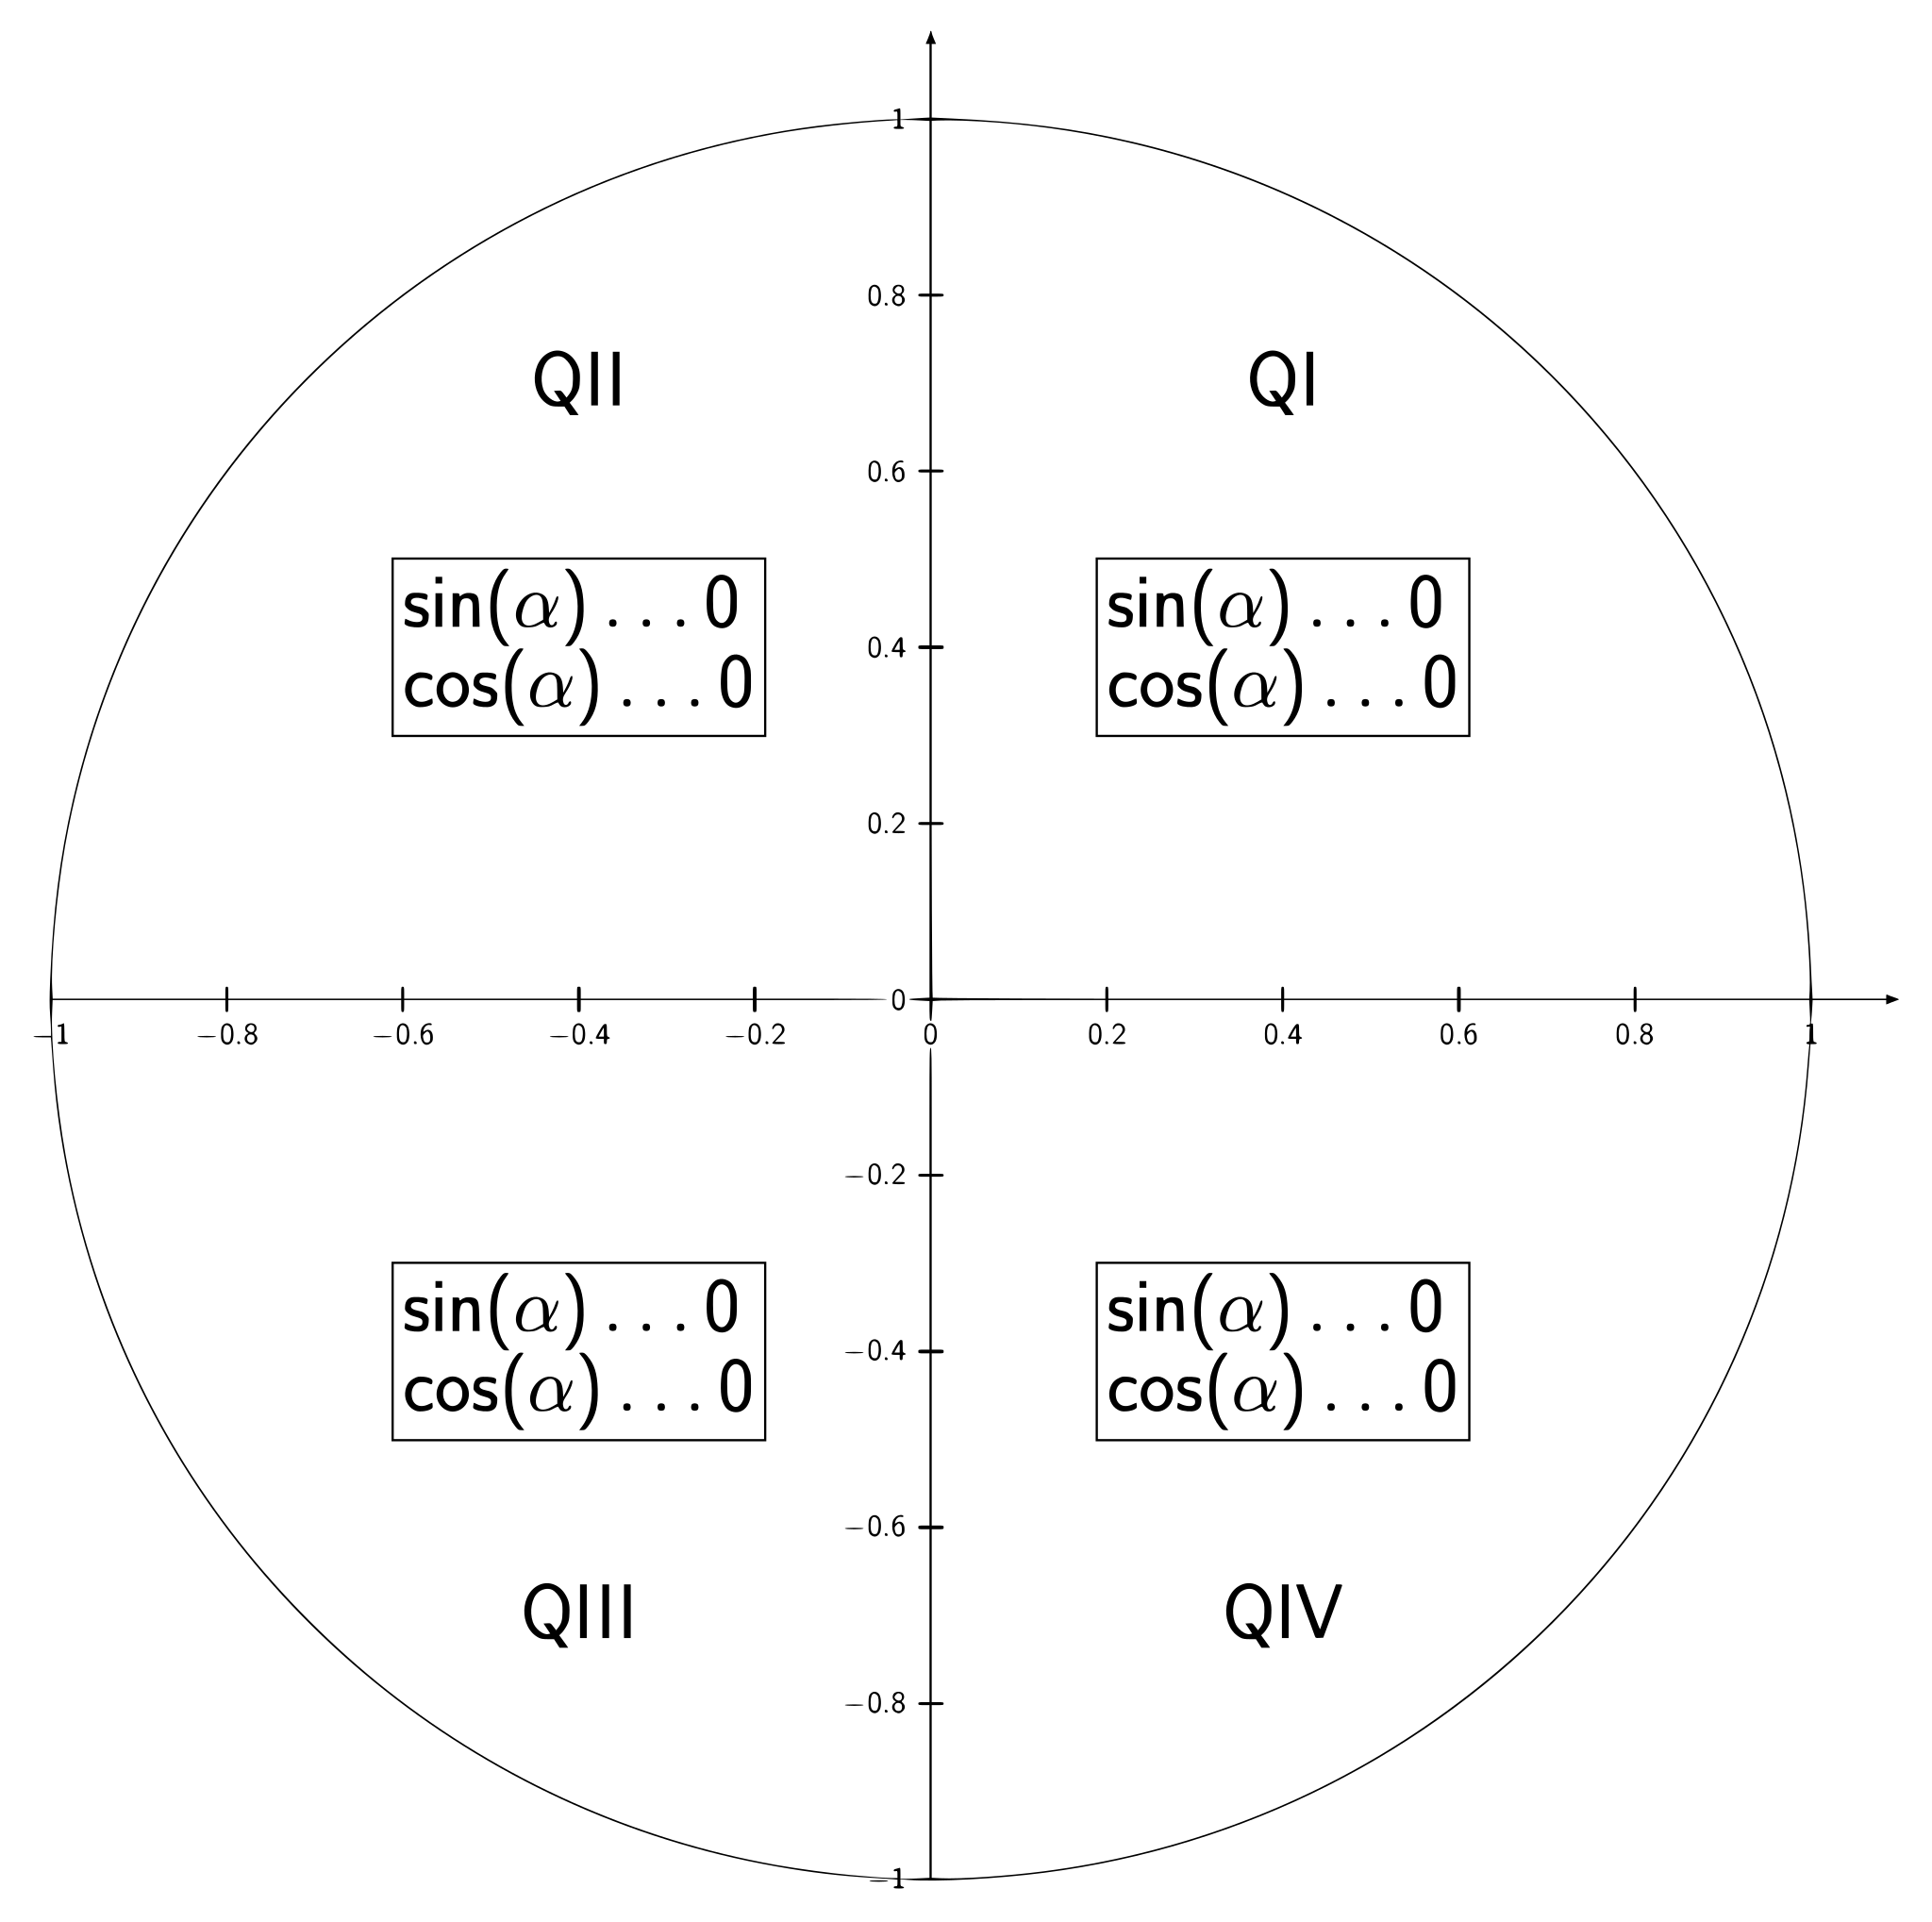
\includegraphics[width=0.4\textwidth,height=\textheight]{figures/fig23.pdf}
\end{center}

\end{exercise}

\subsection{Valeurs extrêmes et valeurs
particulières}\label{valeurs-extruxeames-et-valeurs-particuliuxe8res}

\begin{exercise}[]\protect\hypertarget{exr-valeurs-extr}{}\label{exr-valeurs-extr}

Sur base des dessins de la page précédente, complète les inégalités
suivantes: quel que soit l'angle \(\alpha\in[0^\circ;360^\circ]\)

\[
\makebox[2cm]{\dotfill}\le\cos(\alpha)\le\makebox[2cm]{\dotfill}\text{ et } \makebox[2cm]{\dotfill}\le\sin(\alpha)\le\makebox[2cm]{\dotfill}
\]

\end{exercise}

Tu as rencontré en 3e des valeurs particulières de sinus et cosinus. Ces
valeurs doivent être connues par coeur. \begin{center}
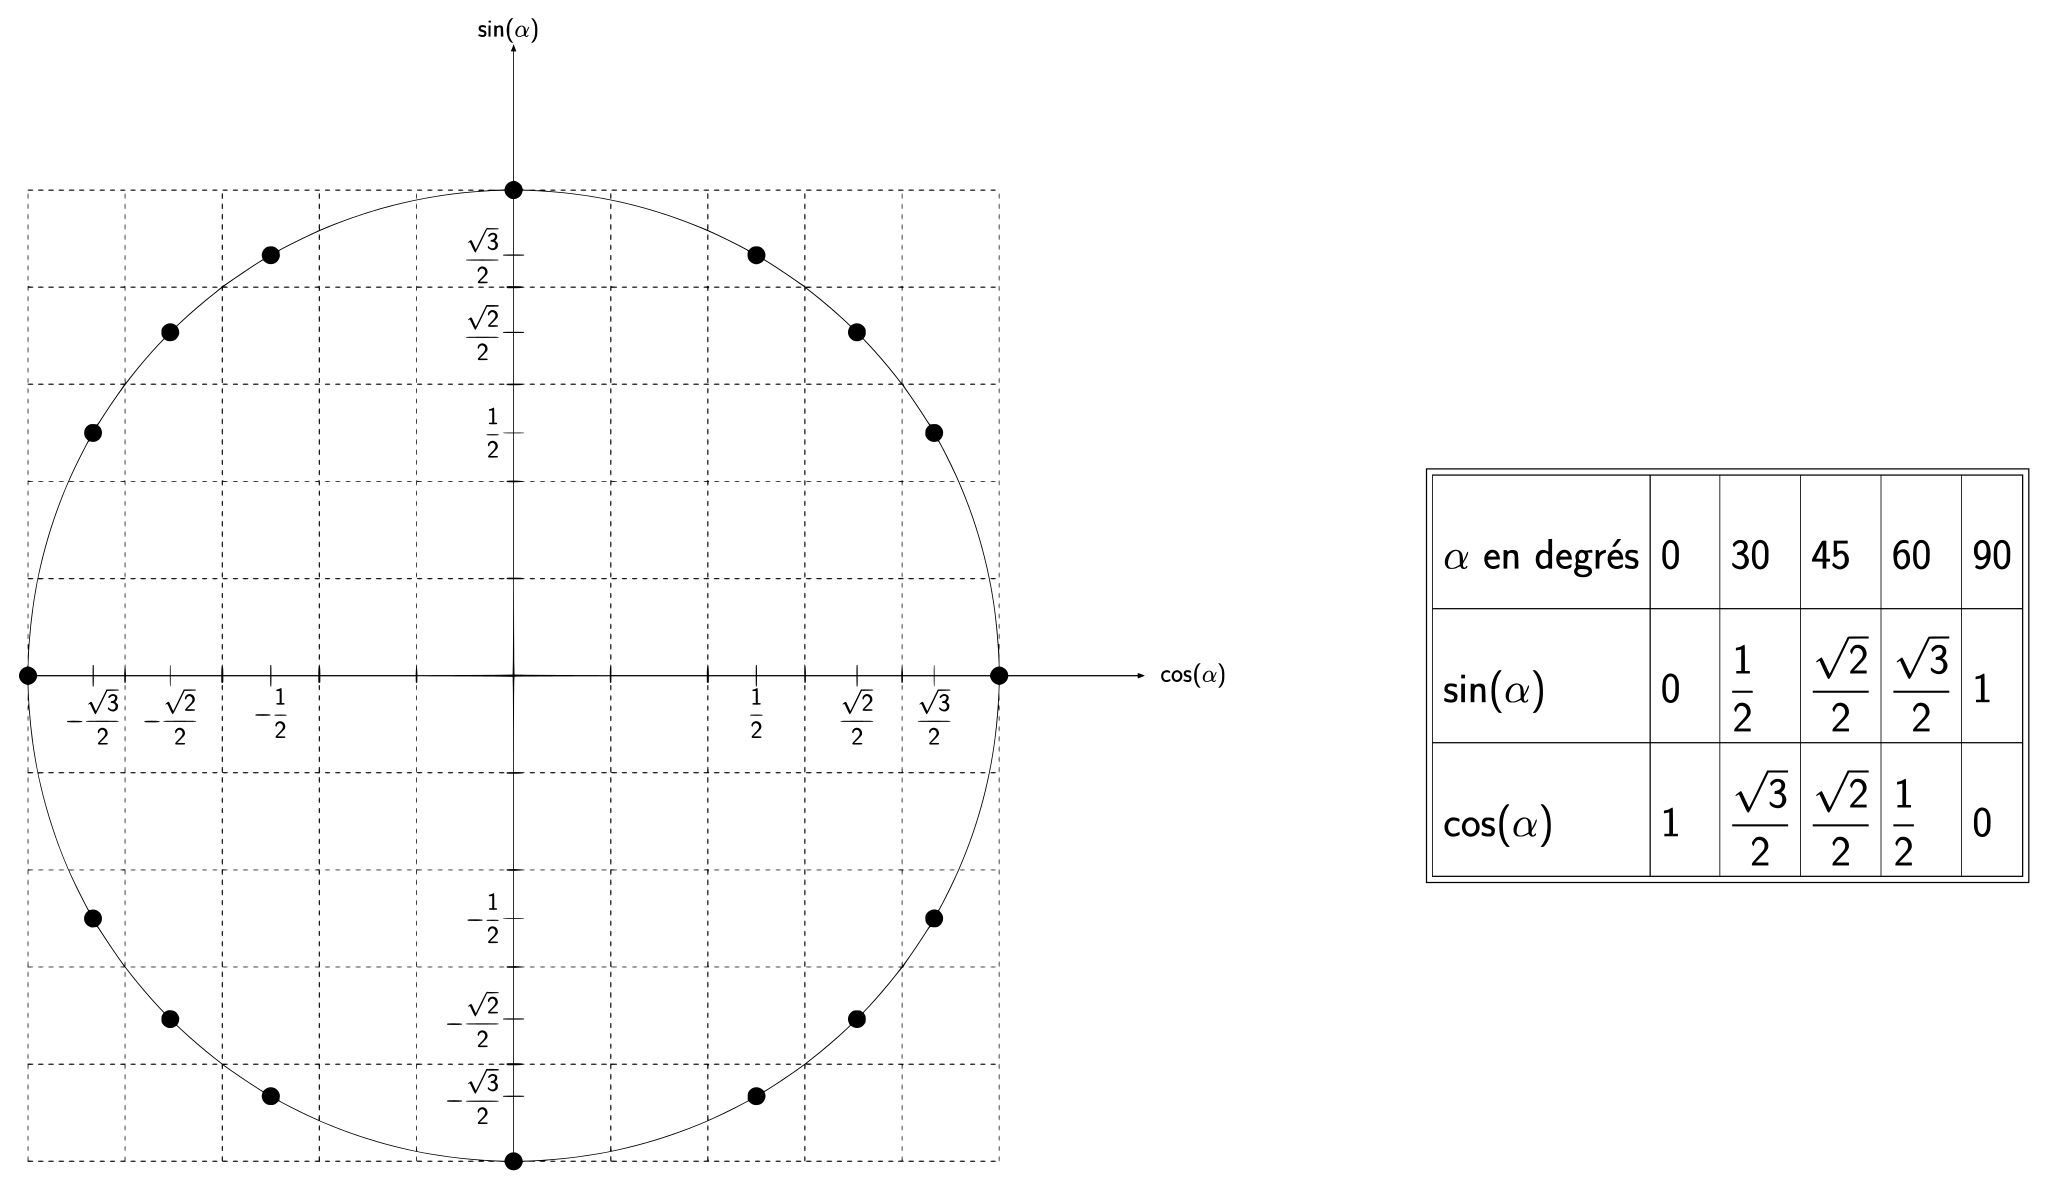
\includegraphics[width=0.8\textwidth,height=\textheight]{figures/fig24.pdf}
\end{center}

\subsection{Utilisation de la
calculatrice}\label{utilisation-de-la-calculatrice}

On a vu au chapitre précédent que la calculatrice permet d'obtenir un
angle étant donné une valeur pour le sinus ou le cosinus, via les
touches \texttt{arcsin} et \texttt{arccos} (parfois notées
\texttt{sin\textsuperscript{-1}} et \texttt{cos\textsuperscript{-1}})

\begin{center}
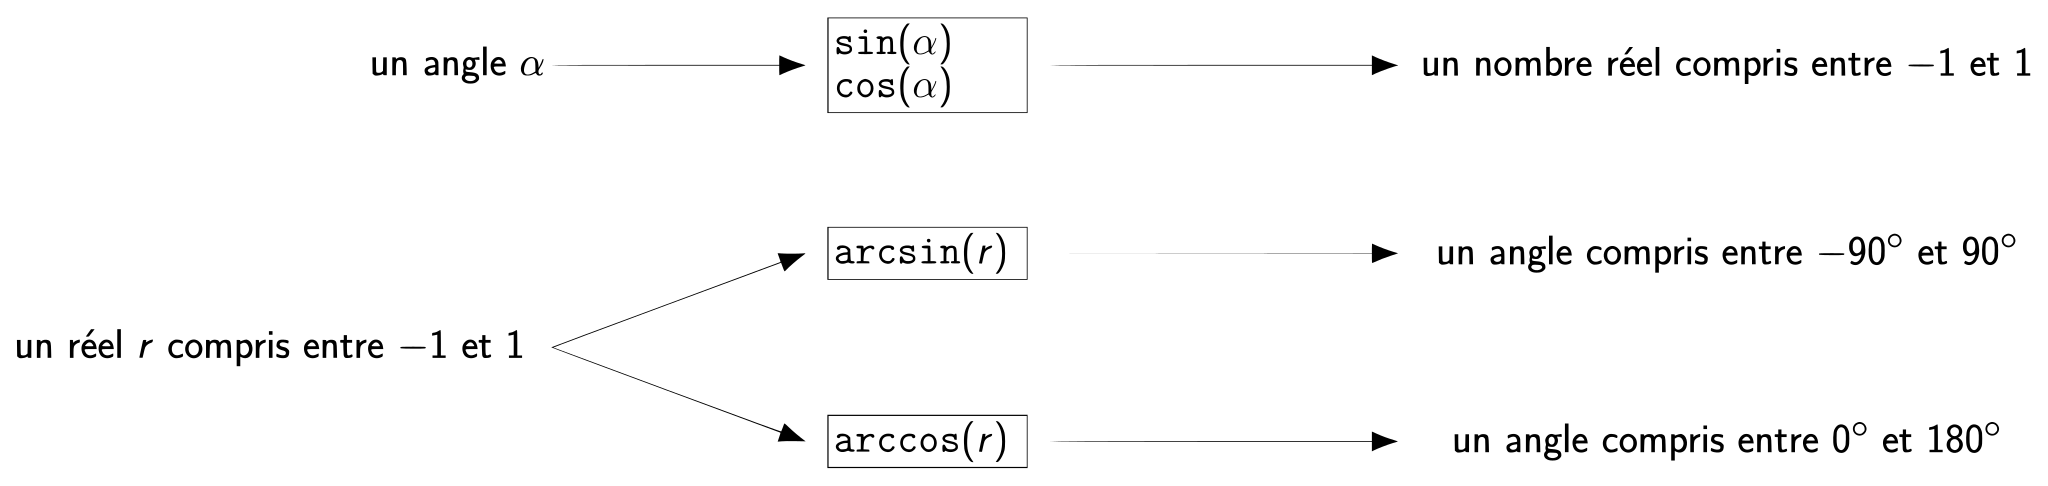
\includegraphics[width=1\textwidth,height=\textheight]{figures/fig25.pdf}
\end{center}

\newpage{}

\subsection{Relation fondamentale}\label{relation-fondamentale}

\begin{theorem}[]\protect\hypertarget{thm-fml-fond}{}\label{thm-fml-fond}

Quel que soit l'angle \(\alpha\in[0^\circ;360^\circ]\),
\(\sin^2(\alpha)+\cos^2(\alpha)=1\)

\end{theorem}

\begin{proof}
La démonstration de cette formule consiste à appliquer le théorème de
Pythagore:

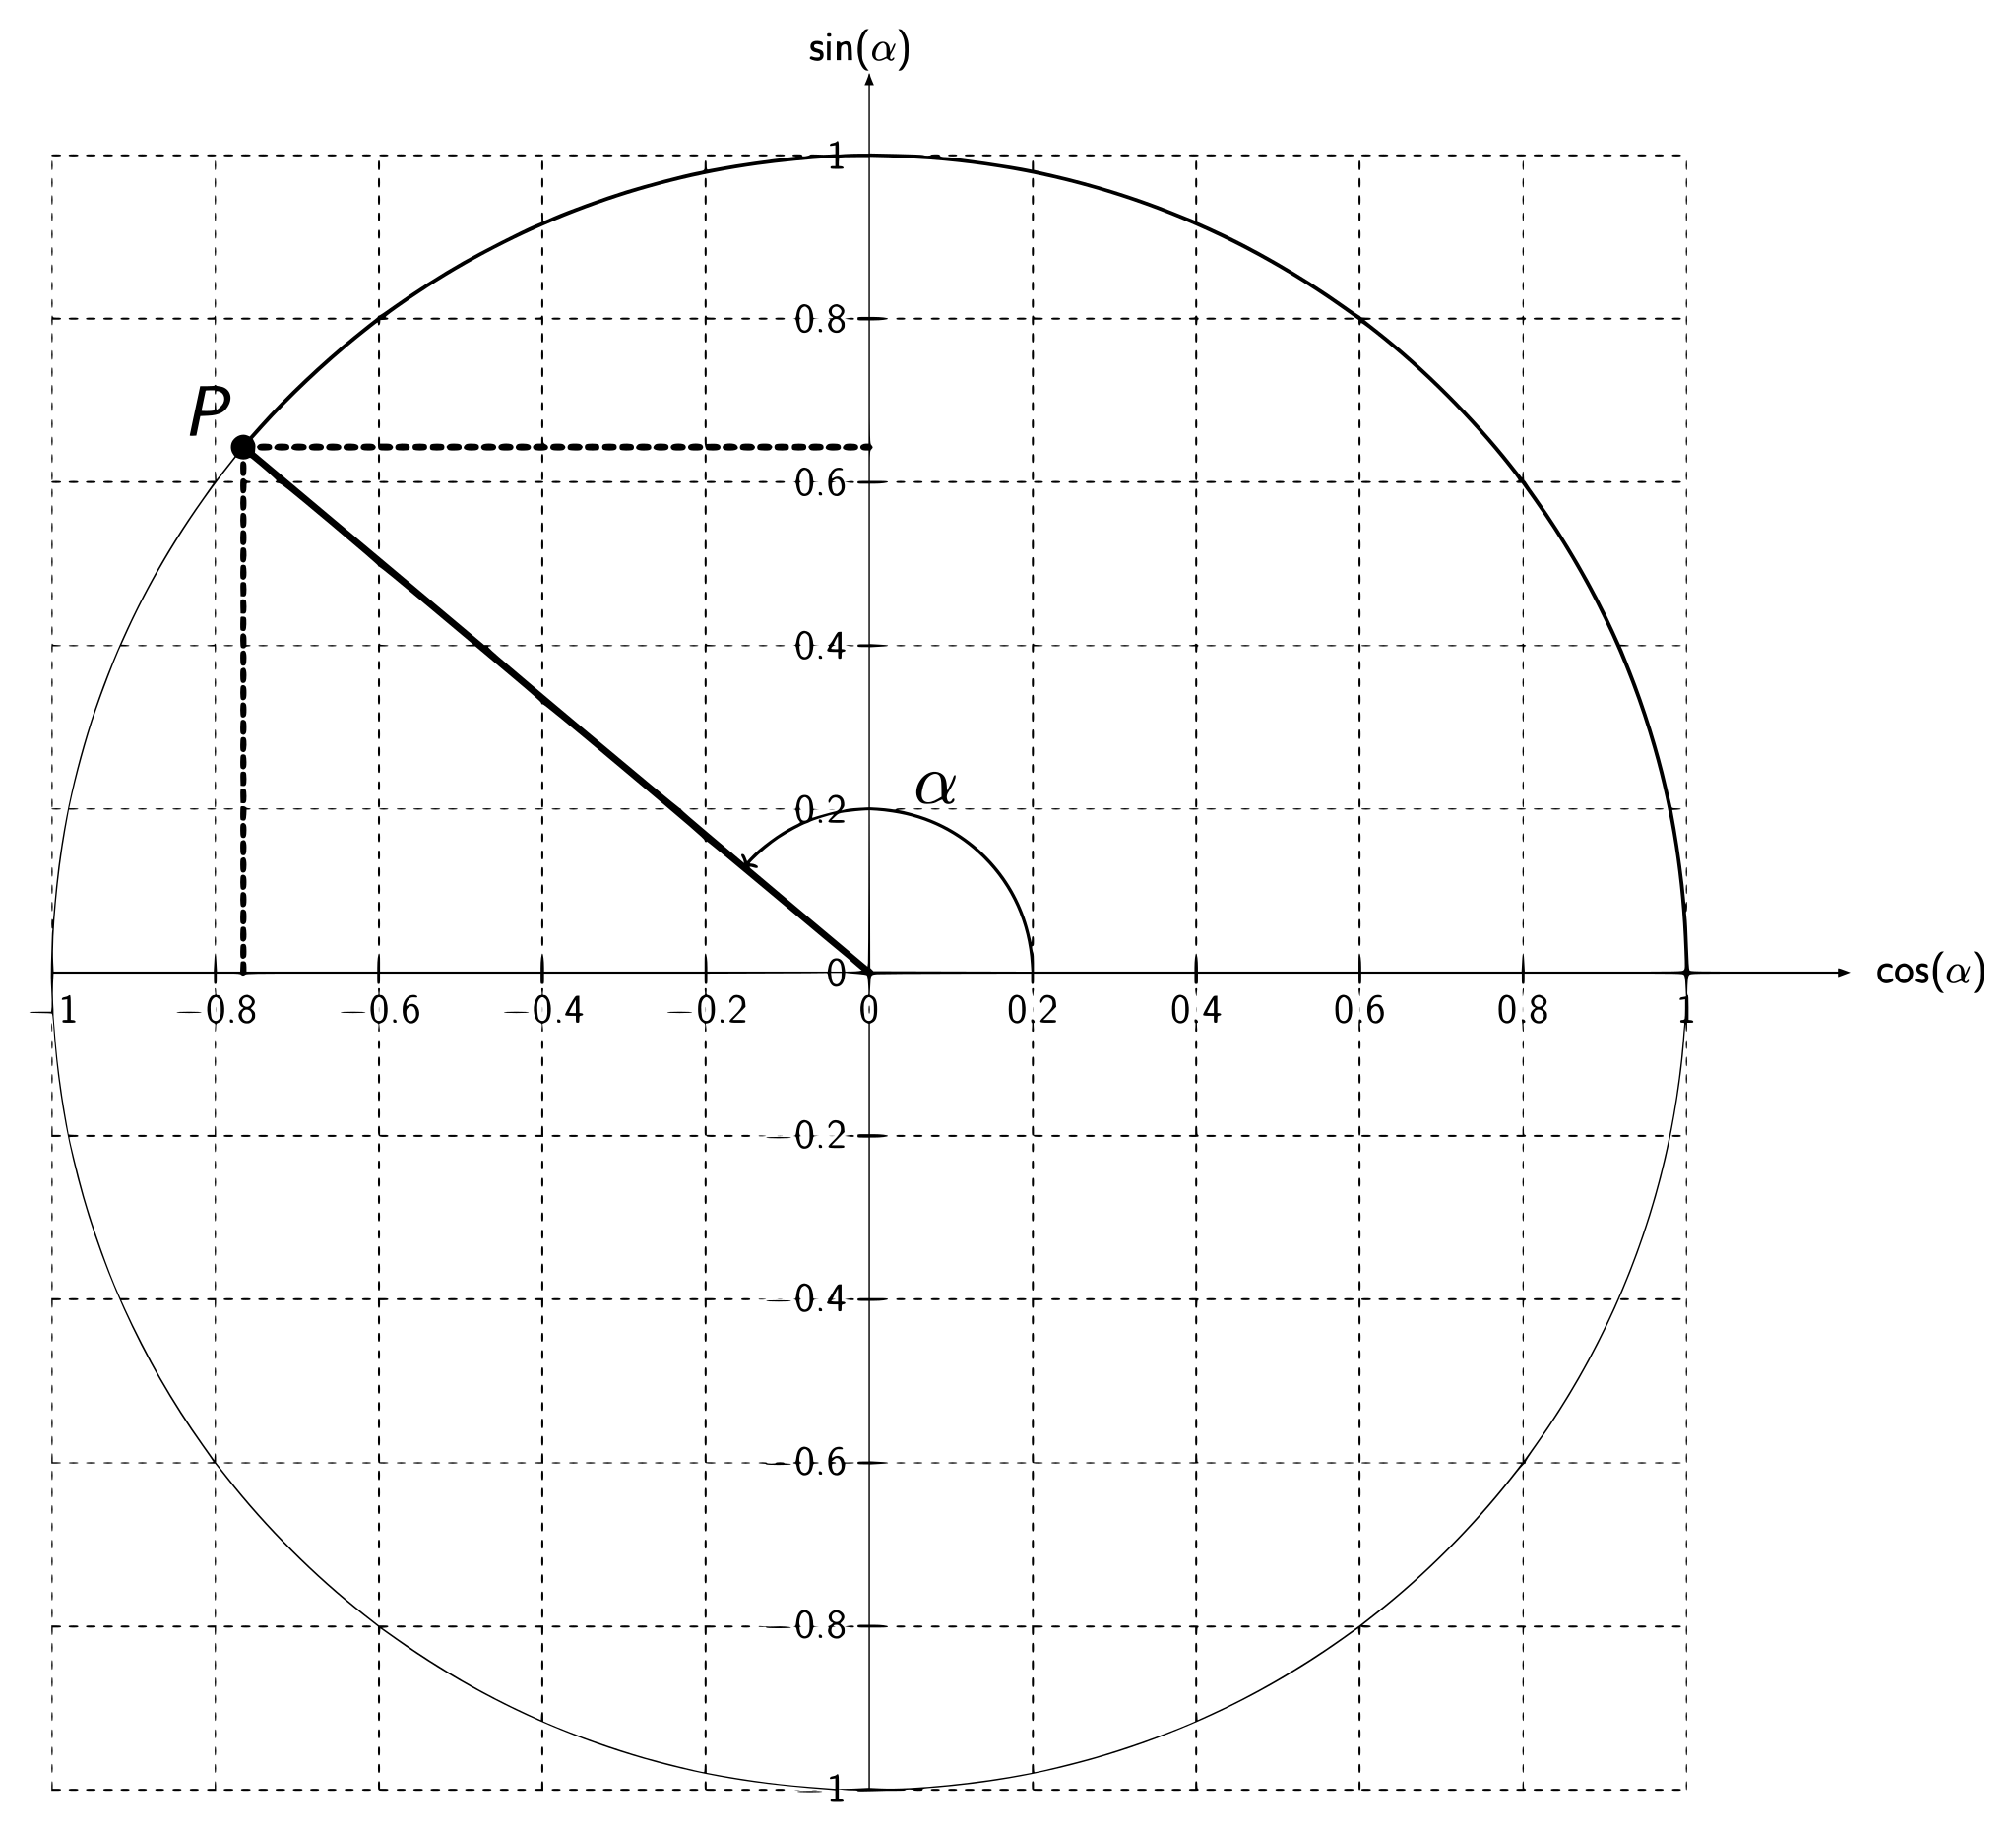
\includegraphics[width=0.5\textwidth,height=\textheight]{figures/fig26.pdf}
\end{proof}

\newpage{}

\subsection{Exercices}\label{exercices-1}

\begin{exercise}[]\protect\hypertarget{exr-}{}\label{exr-}

Représente sur le cercle trigonométrique les angles d'amplitude 20°,
-20°, 120°, -90°, -180°, 225° et 330° ainsi que leur sinus et leur
cosinus.

\begin{center}
\includegraphics[width=1\textwidth,height=\textheight]{figures/fig27.pdf}
\end{center}

\end{exercise}

\newpage{}

\begin{exercise}[]\protect\hypertarget{exr-}{}\label{exr-}

Vrai ou faux ? Justifie.

\begin{figure}

\begin{minipage}{0.60\linewidth}

\begin{enumerate}
\def\labelenumi{\arabic{enumi})}
\item
  Si \(90^\circ<\alpha <180^\circ\), alors \(\cos(\alpha)<0\).
\item
  Si \(270^\circ<\alpha <360^\circ\), alors \(\sin(\alpha)>0\).
\item
  Si \(180^\circ<\alpha <270^\circ\), alors \(\sin(\alpha)\) est
  négatif.
\end{enumerate}

\end{minipage}%
%
\begin{minipage}{0.40\linewidth}
\begin{center}
\includegraphics{figures/fig28.pdf}
\end{center}
\end{minipage}%

\end{figure}%

\end{exercise}

\begin{exercise}[]\protect\hypertarget{exr-quad}{}\label{exr-quad}

Dans quel quadrant se trouve \(\alpha\) sachant que:

\begin{figure}

\begin{minipage}{0.60\linewidth}

\begin{enumerate}
\def\labelenumi{\arabic{enumi})}
\item
  \(\sin(\alpha)<0\) et \(\cos(\alpha)<0\)?
\item
  \(\sin(\alpha)<0\) et \(\cos(\alpha)>0\)?
\item
  \(\sin(\alpha)>0\) et \(\cos(\alpha)>0\)?
\end{enumerate}

\end{minipage}%
%
\begin{minipage}{0.40\linewidth}
\begin{center}
\includegraphics{figures/fig28.pdf}
\end{center}
\end{minipage}%

\end{figure}%

\end{exercise}

\begin{exercise}[]\protect\hypertarget{exr-}{}\label{exr-}

Complète par \(=\) ou \(\neq\).

\begin{figure}

\begin{minipage}{0.70\linewidth}

\begin{enumerate}
\def\labelenumi{\arabic{enumi})}
\item
  \(\sin(20)\makebox[2cm]{\dotfill}\sin(120)\)
\item
  \(\cos(60)\makebox[2cm]{\dotfill}\sin(30)\)
\item
  \(\cos(160)\makebox[2cm]{\dotfill}-\cos(20)\)
\end{enumerate}

\end{minipage}%
%
\begin{minipage}{0.30\linewidth}
\begin{center}
\includegraphics{figures/fig28.pdf}
\end{center}
\end{minipage}%

\end{figure}%

\end{exercise}

\newpage{}

\begin{exercise}[]\protect\hypertarget{exr-}{}\label{exr-}

Représente sur les cercles trigonométriques ci-dessous les angles
correspondants aux informations données.

\begin{center}
\includegraphics[width=1\textwidth,height=\textheight]{figures/fig29.pdf}
\end{center}

\end{exercise}

\newpage{}

\begin{exercise}[]\protect\hypertarget{exr-}{}\label{exr-}

Détermine l'amplitude des angles (entre 0° et 360°) dont les nombres
trigonométriques sont donnés ci-dessous après avoir visualisé la
situation sur le cercle trigonométrique. Arrondis au dixième près si
nécessaire.

\begin{center}
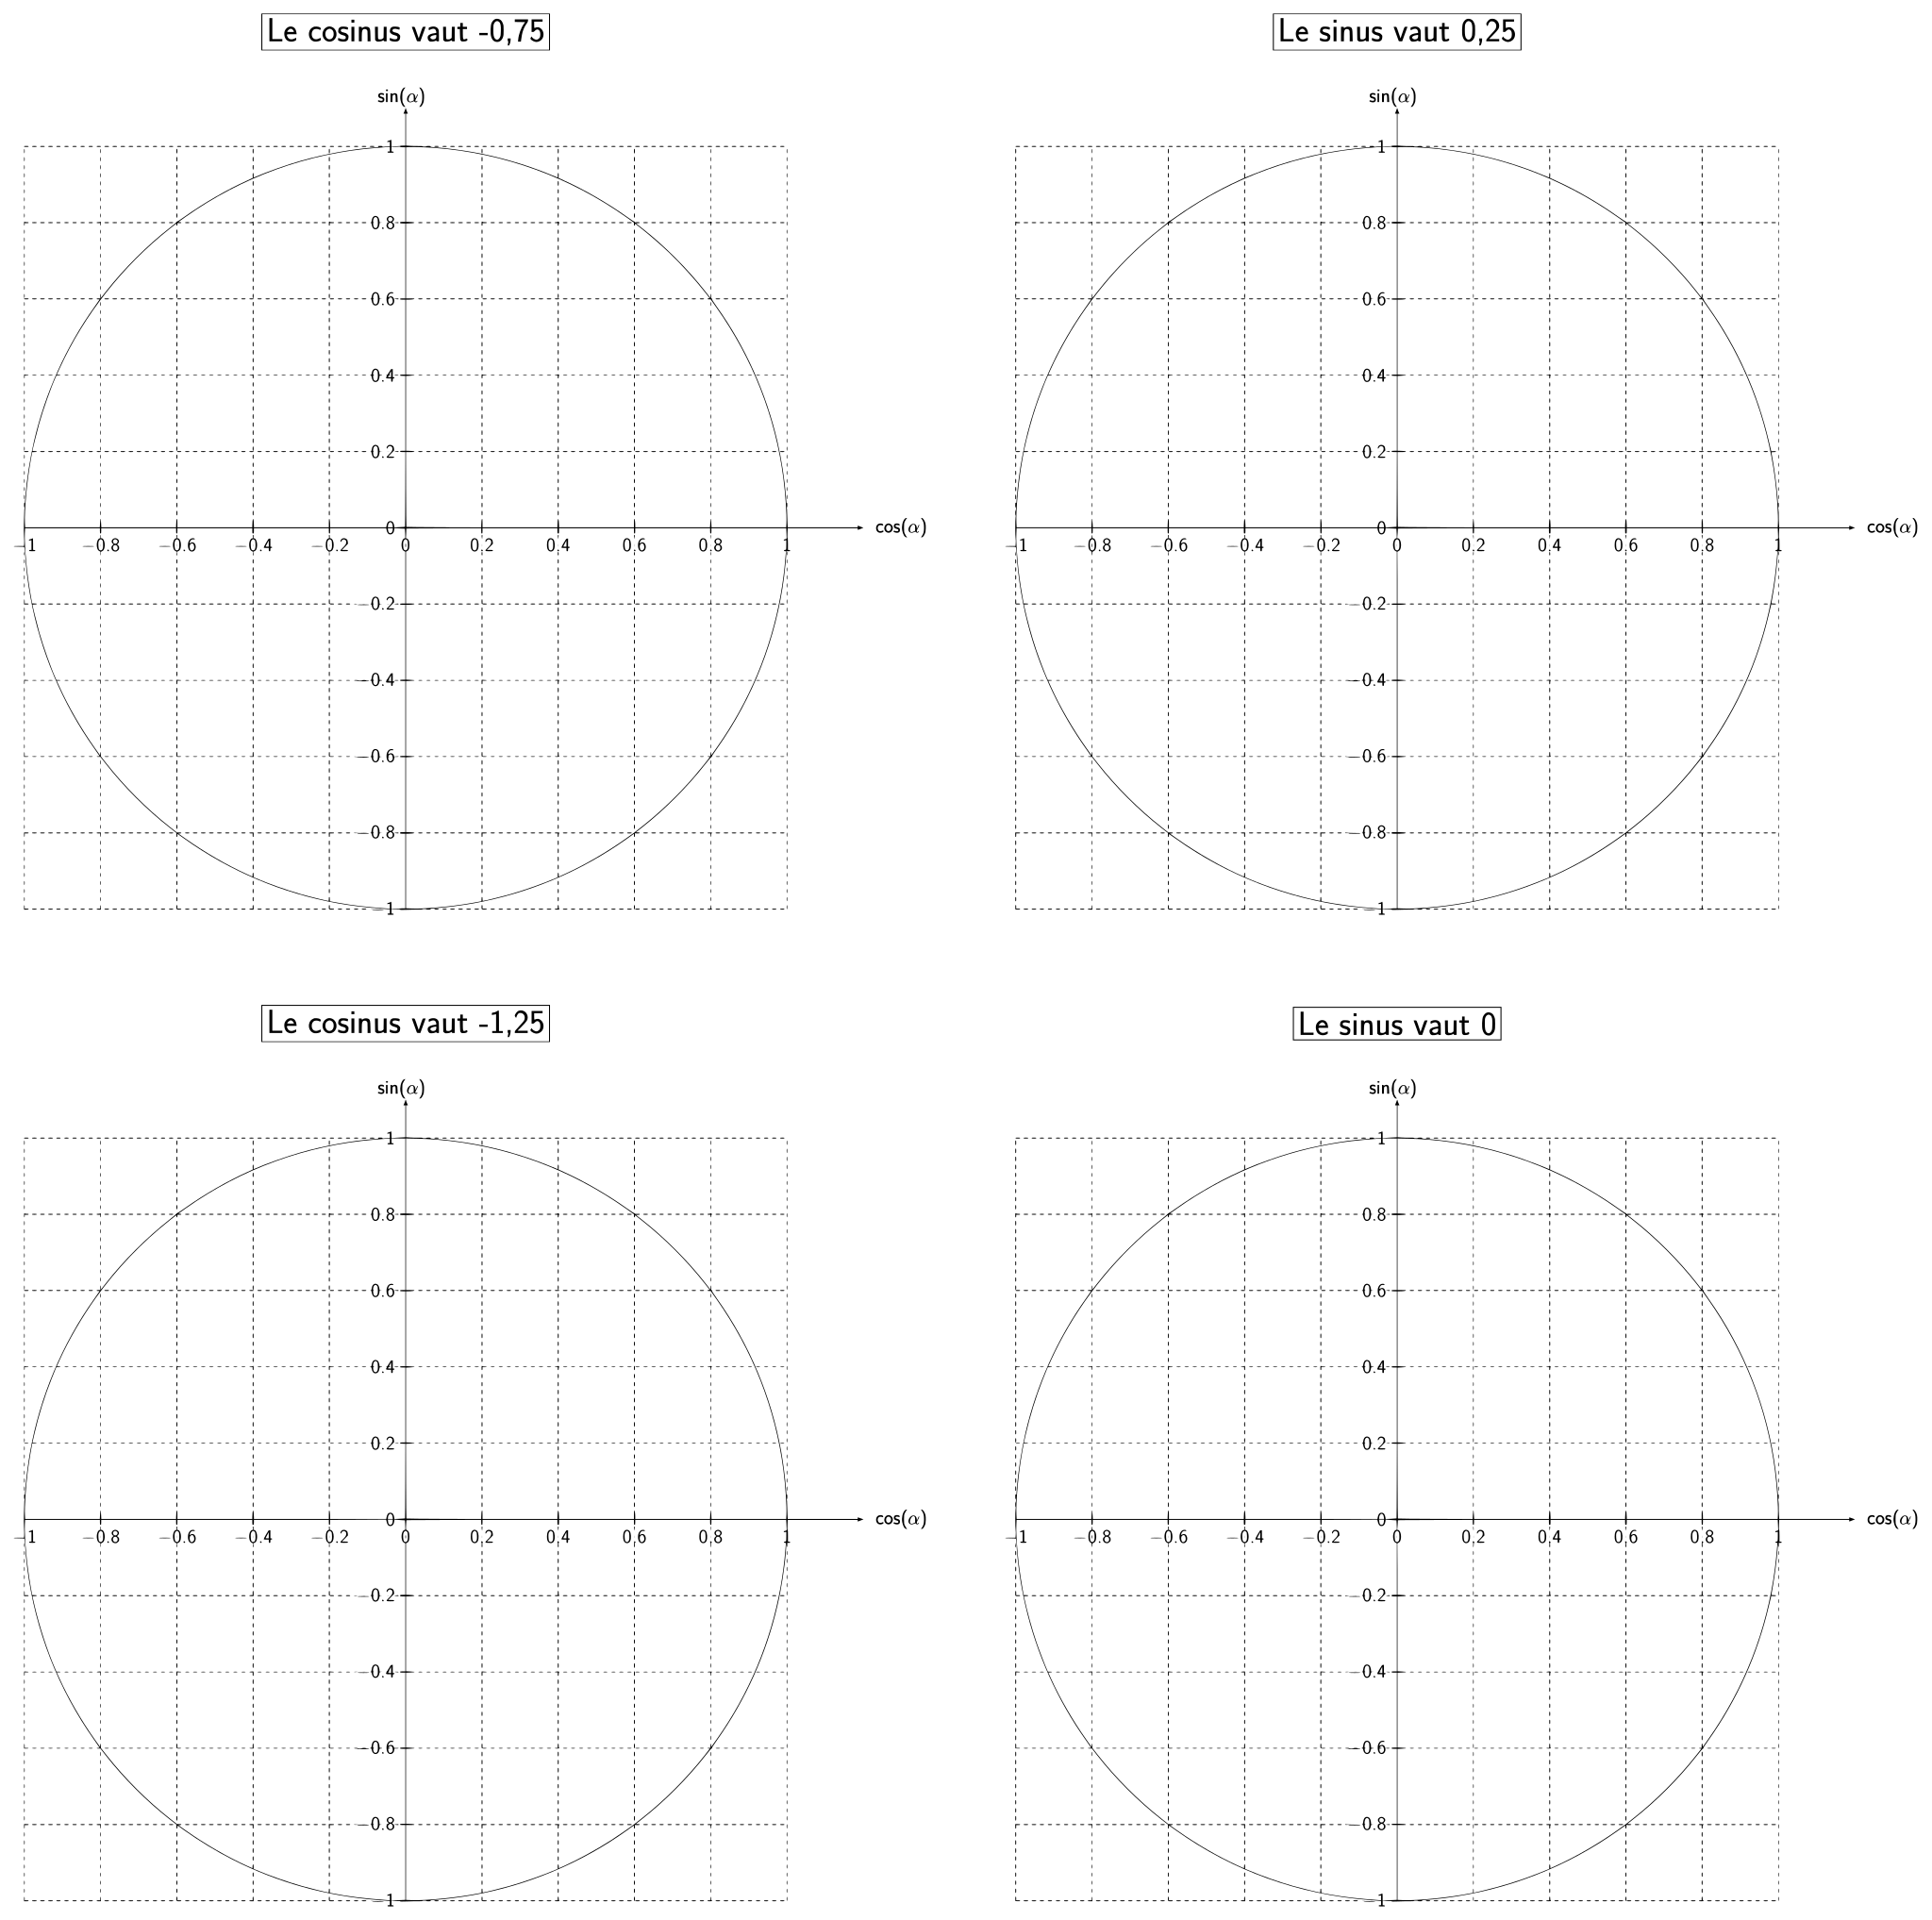
\includegraphics[width=1\textwidth,height=\textheight]{figures/fig30.pdf}
\end{center}

\end{exercise}

\newpage{}

\begin{exercise}[]\protect\hypertarget{exr-}{}\label{exr-}

Sachant que \(\cos(60^\circ) = \dfrac{1}{2}\) , complète les égalités
suivantes (commence par représenter tous les angles dans le cercle
trigonométrique).

\begin{figure}

\begin{minipage}{0.60\linewidth}

\begin{enumerate}
\def\labelenumi{\arabic{enumi})}
\item
  \(\cos(-60)=\makebox[2cm]{\dotfill}\)
\item
  \(\cos(120)=\makebox[2cm]{\dotfill}\)
\item
  \(\cos(300)=\makebox[2cm]{\dotfill}\)
\item
  \(\cos(240)=\makebox[2cm]{\dotfill}\)
\end{enumerate}

\end{minipage}%
%
\begin{minipage}{0.40\linewidth}
\begin{center}
\includegraphics{figures/fig28.pdf}
\end{center}
\end{minipage}%

\end{figure}%

\end{exercise}

\begin{exercise}[]\protect\hypertarget{exr-}{}\label{exr-}

Sachant que \(\sin(45^\circ) = \dfrac{\sqrt{2}}{2}\) , complète les
égalités suivantes (commence par représenter tous les angles dans le
cercle trigonométrique).

\begin{figure}

\begin{minipage}{0.60\linewidth}

\begin{enumerate}
\def\labelenumi{\arabic{enumi})}
\item
  \(\sin(-45)=\makebox[2cm]{\dotfill}\)
\item
  \(\sin(135)=\makebox[2cm]{\dotfill}\)
\item
  \(\sin(225)=\makebox[2cm]{\dotfill}\)
\item
  \(\sin(315)=\makebox[2cm]{\dotfill}\)
\end{enumerate}

\end{minipage}%
%
\begin{minipage}{0.40\linewidth}
\begin{center}
\includegraphics{figures/fig28.pdf}
\end{center}
\end{minipage}%

\end{figure}%

\end{exercise}

\begin{exercise}[]\protect\hypertarget{exr-}{}\label{exr-}

Sachant que \(\alpha\in\text{QII}\) et que
\(\sin(\alpha) = \dfrac{4}{5}\), calcule la valeur exacte de
\(\cos(\alpha)\) en utilisant la formule fondamentale de trigonométrie.

\end{exercise}

\begin{exercise}[]\protect\hypertarget{exr-}{}\label{exr-}

Sachant que \(\alpha\in\text{QIII}\) et que
\(\cos(\alpha) = \dfrac{-2}{3}\), calcule la valeur exacte de
\(\sin(\alpha)\) en utilisant la formule fondamentale de trigonométrie.

\end{exercise}

\newpage{}

\section{Tangente dans le cercle
trigonométrique}\label{tangente-dans-le-cercle-trigonomuxe9trique}

\subsection{Introduction: la tangente dans le premier
quadrant}\label{introduction-la-tangente-dans-le-premier-quadrant}

Tu as vu en 3e une définition de la tangente d'un angle dans un triangle
rectangle.

\begin{center}
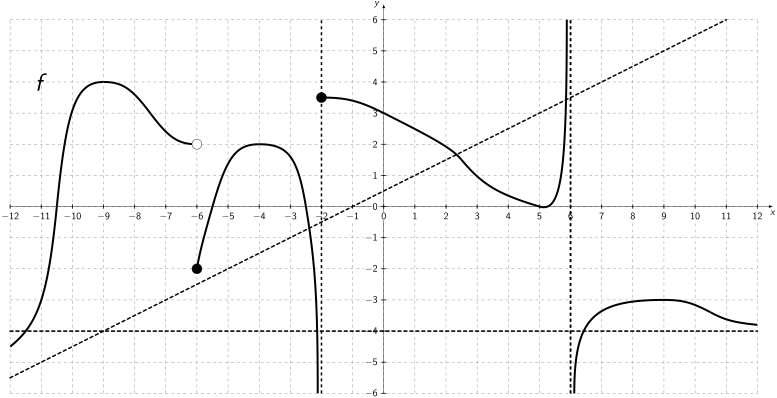
\includegraphics[width=0.5\textwidth,height=\textheight]{figures/fig3.pdf}
\end{center}

Le but de ce chapitre est de définir la tangente d'un angle, au delà des
angles aigus. Nous allons d'abord analyser la situation des angles aigus
dans le cercle trigonométrique, puis généraliser pour les angles obtus.

\begin{center}
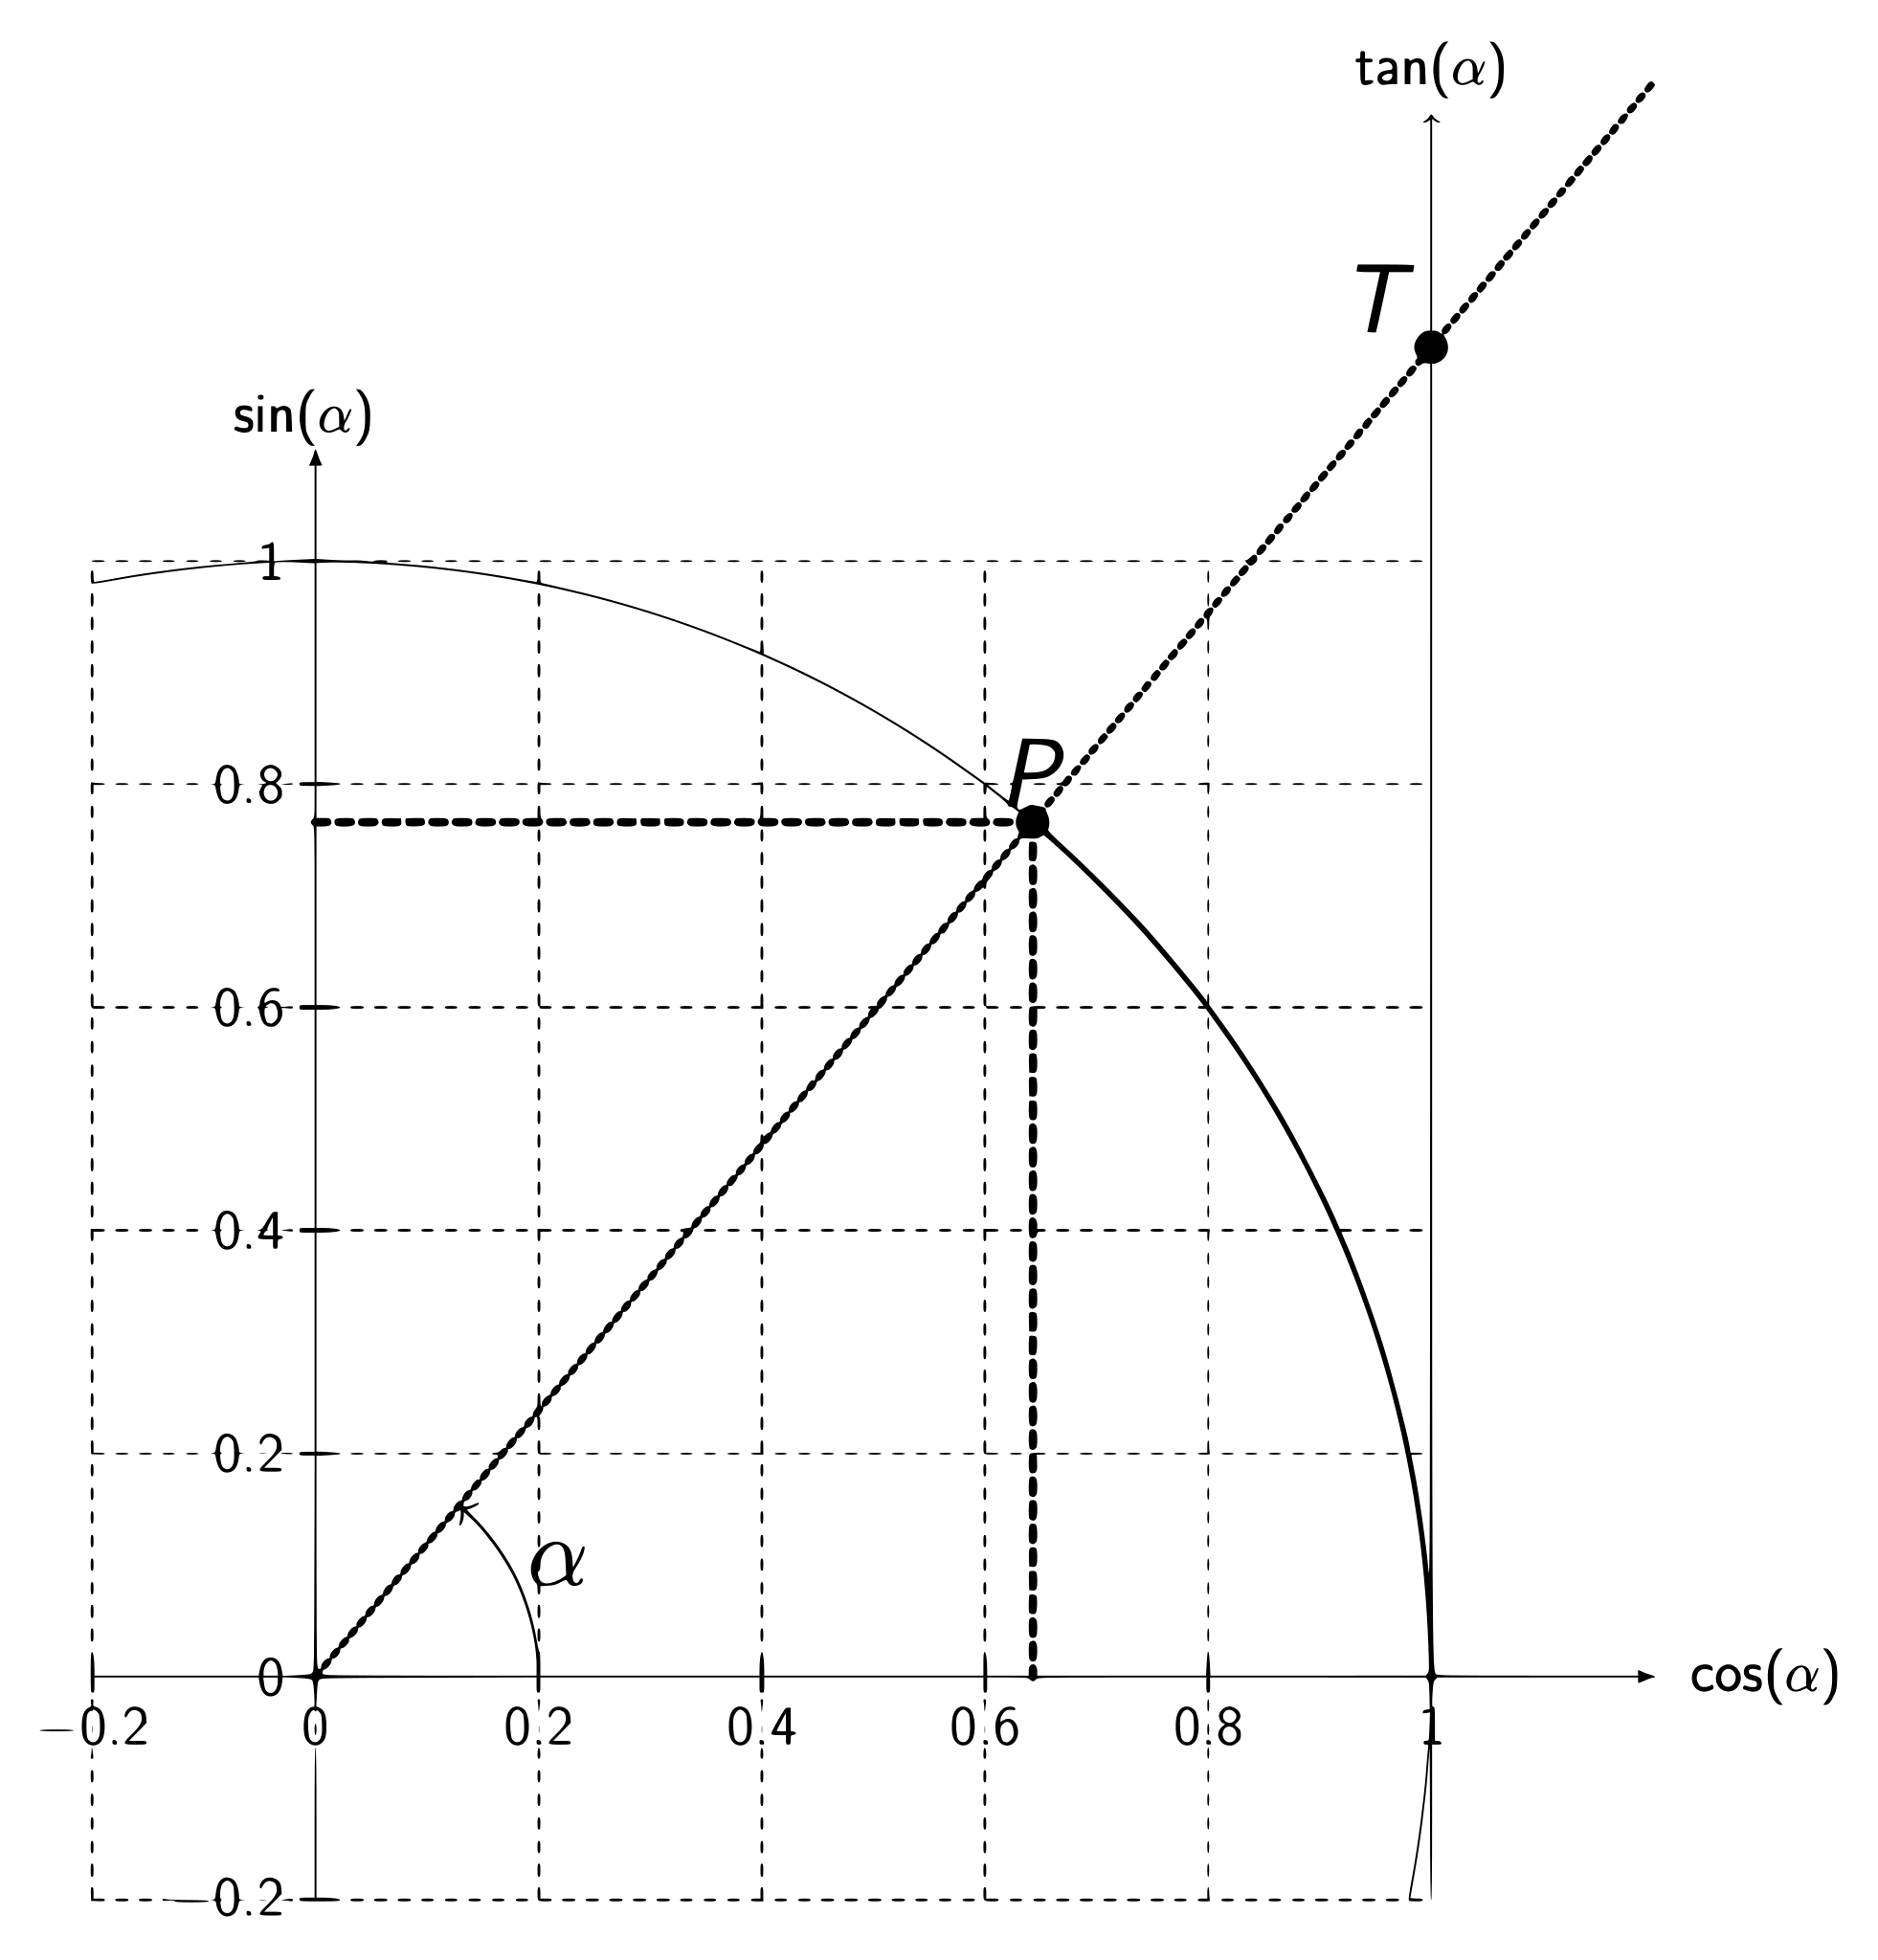
\includegraphics[width=0.5\textwidth,height=\textheight]{figures/fig36.pdf}
\end{center}

Sur cette figure, on observe deux triangles rectangles: le triangle
\(OPA\), rectangle en \(A\) et \(OTB\), rectangle en \(B\). On peut donc
calculer la tangente de \(\alpha\) dans ces deux triangles:

\begin{enumerate}
\def\labelenumi{\arabic{enumi})}
\item
  dans \(OPA\), \(\tan(\alpha)=\)
\item
  dans \(OTB\), \(\tan(\alpha)=\)
\end{enumerate}

Ainsi, pour calculer la tangente, il suffit de calculer \dotfill.

En effet, le calcul de la tangente d'un angle de dépend pas du triangle
rectangle dans lequel on trouve l'angle \(\alpha\).

De plus, on ré-observe un lien fort entre la tangente, le sinus et le
cosinus: \(\tan(\alpha)=\dfrac{\sin(\alpha)}{\cos(\alpha)}\). Donc pour
calculer la tangente, on peut utiliser les autres nombres
trigonométriques!

\subsection{Définition}\label{duxe9finition-1}

\begin{definition}[]\protect\hypertarget{def-tan}{}\label{def-tan}

Soit \(\alpha\) un angle et \(P\) le point correspondant sur le cercle
trigonométrique. Soit \(T\) le point d'intersection entre la droite
\(OP\) et l'axe des tangentes (la droite verticale passant par le point
\((1;0)\)). Alors, \(\tan(\alpha)\) est l'ordonnée du point \(T\).
\begin{center}
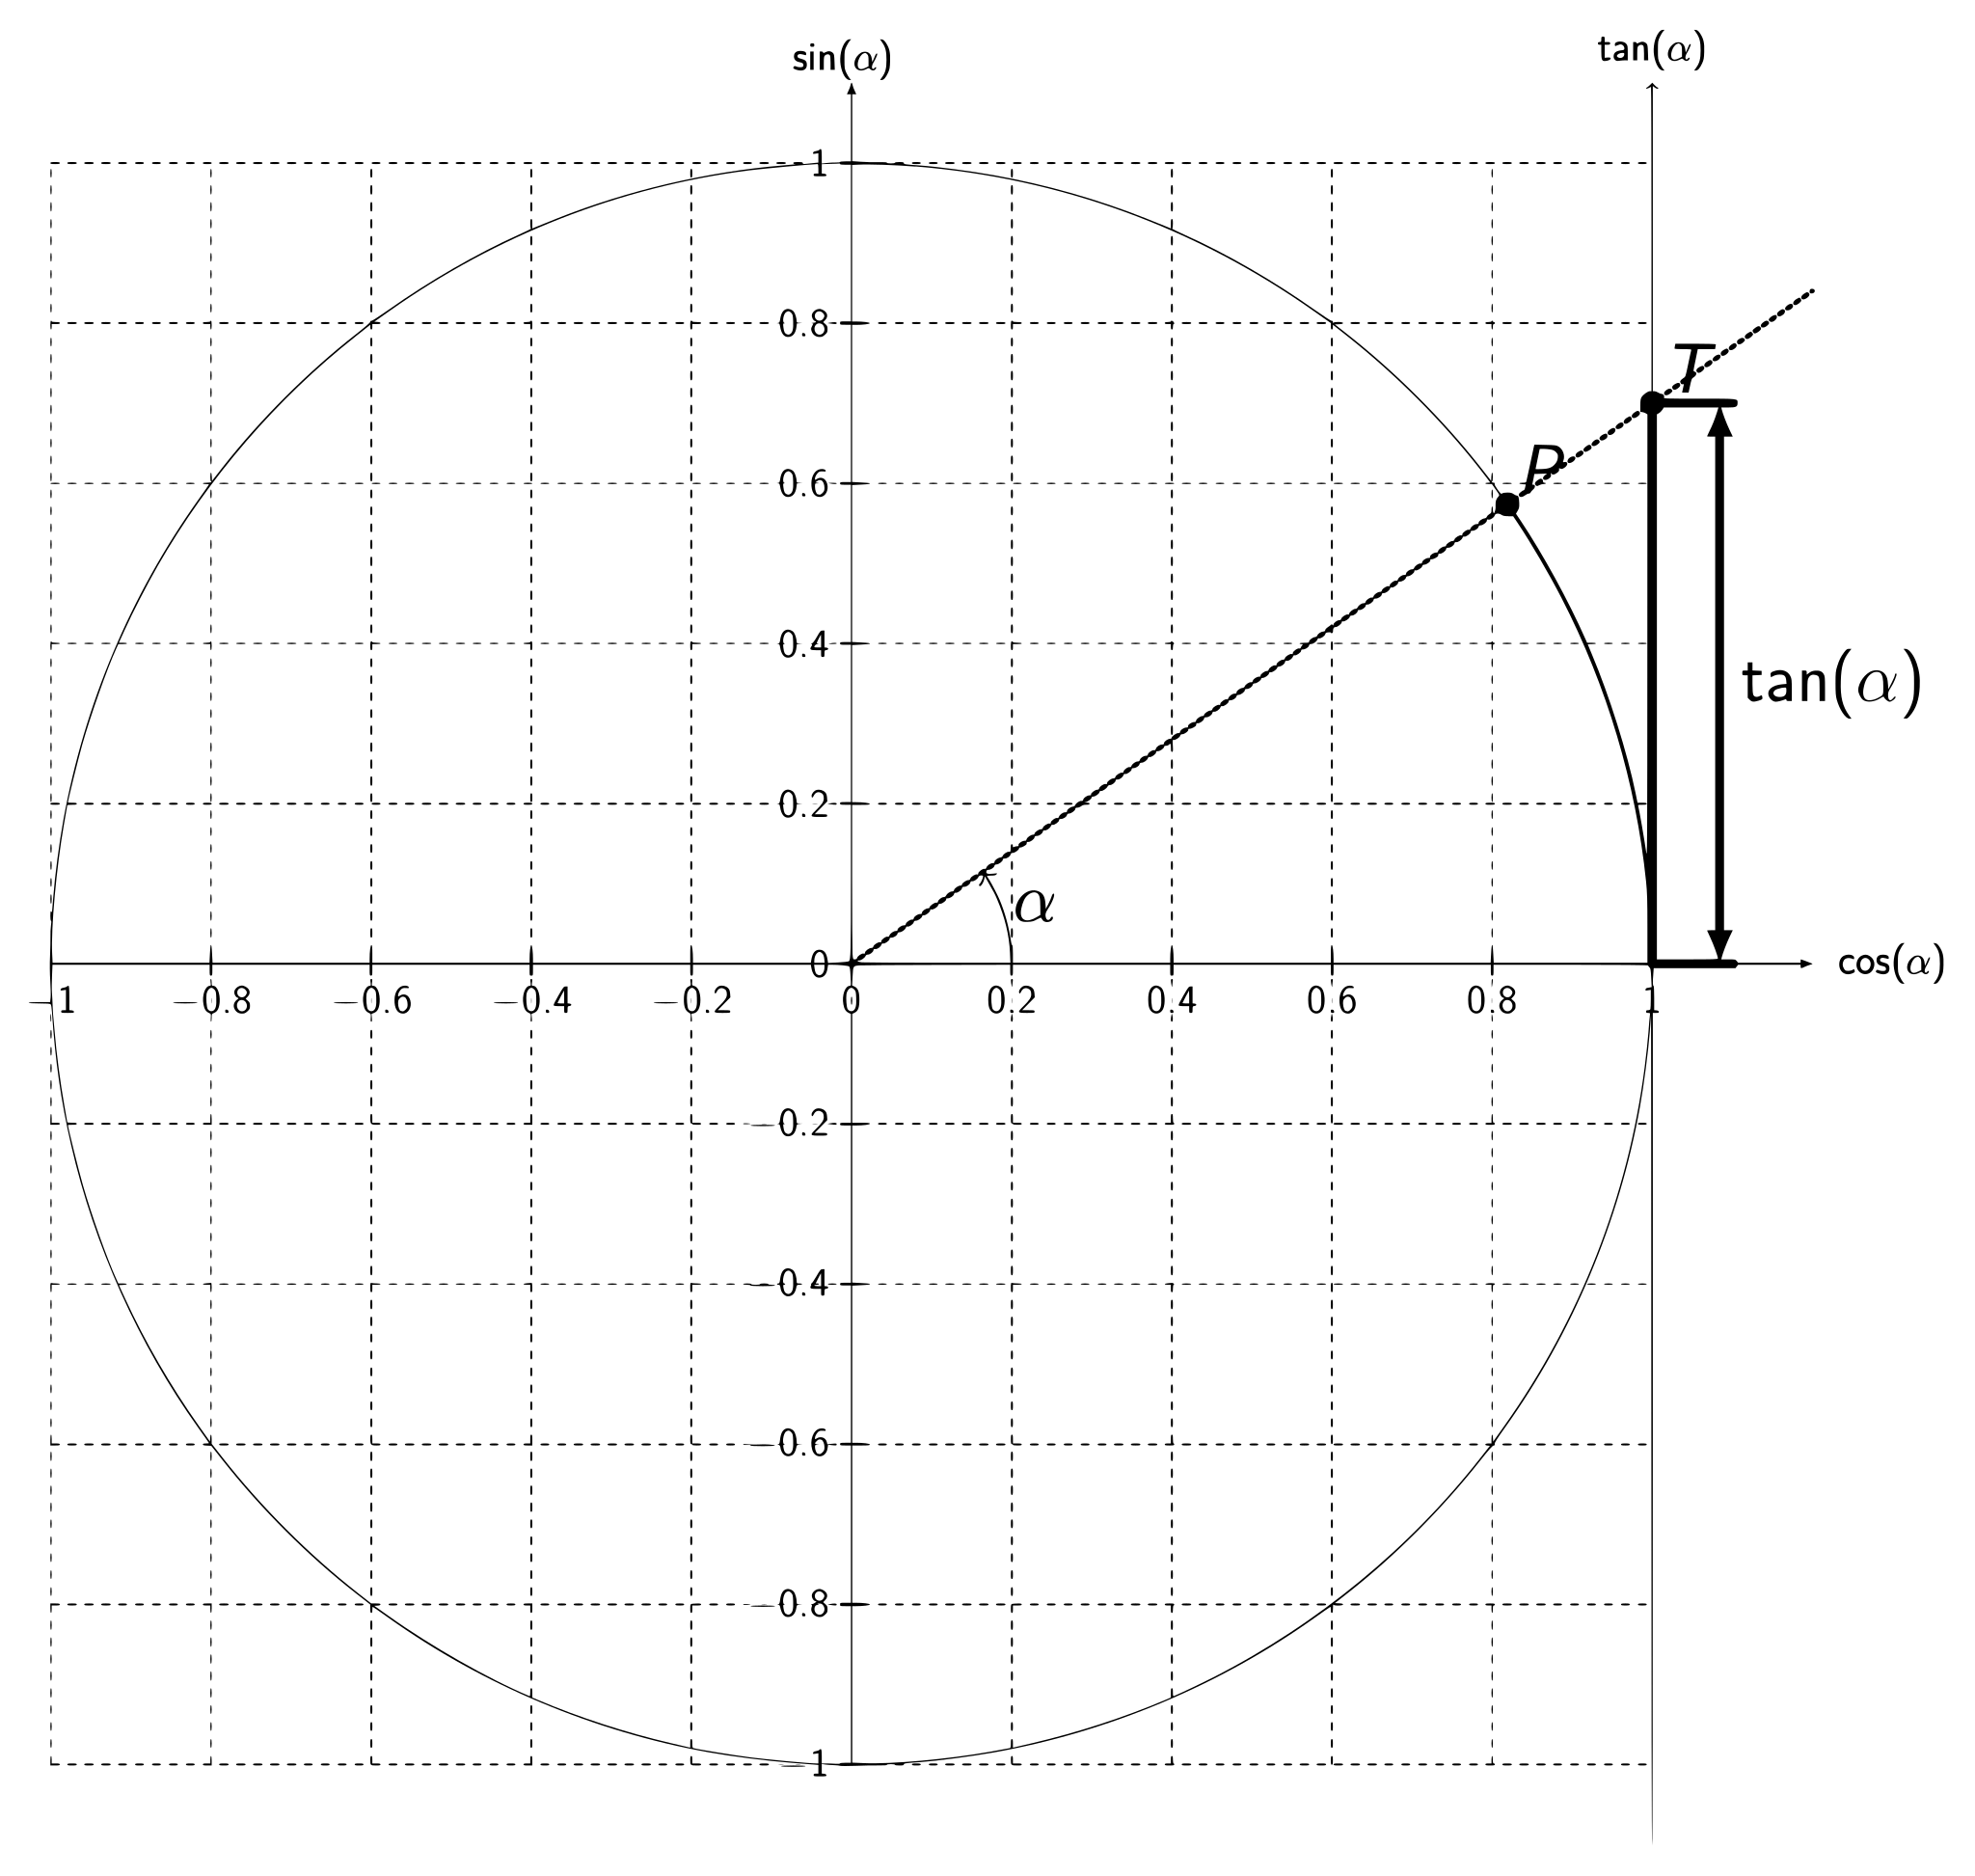
\includegraphics[width=0.4\textwidth,height=\textheight]{figures/fig32.pdf}
\end{center}

\end{definition}

\begin{tcolorbox}[enhanced jigsaw, bottomrule=.15mm, colback=white, bottomtitle=1mm, toprule=.15mm, colbacktitle=quarto-callout-important-color!10!white, breakable, title=\textcolor{quarto-callout-important-color}{\faExclamation}\hspace{0.5em}{Condition d'existence}, arc=.35mm, left=2mm, toptitle=1mm, coltitle=black, rightrule=.15mm, opacityback=0, leftrule=.75mm, colframe=quarto-callout-important-color-frame, opacitybacktitle=0.6, titlerule=0mm]

La tangente d'un angle n'existe pas toujours. En effet pour les angles
\(90^\circ\) et \(270^\circ\), il n'est pas possible de construire une
intersection avec l'axe des tangentes. \begin{center}
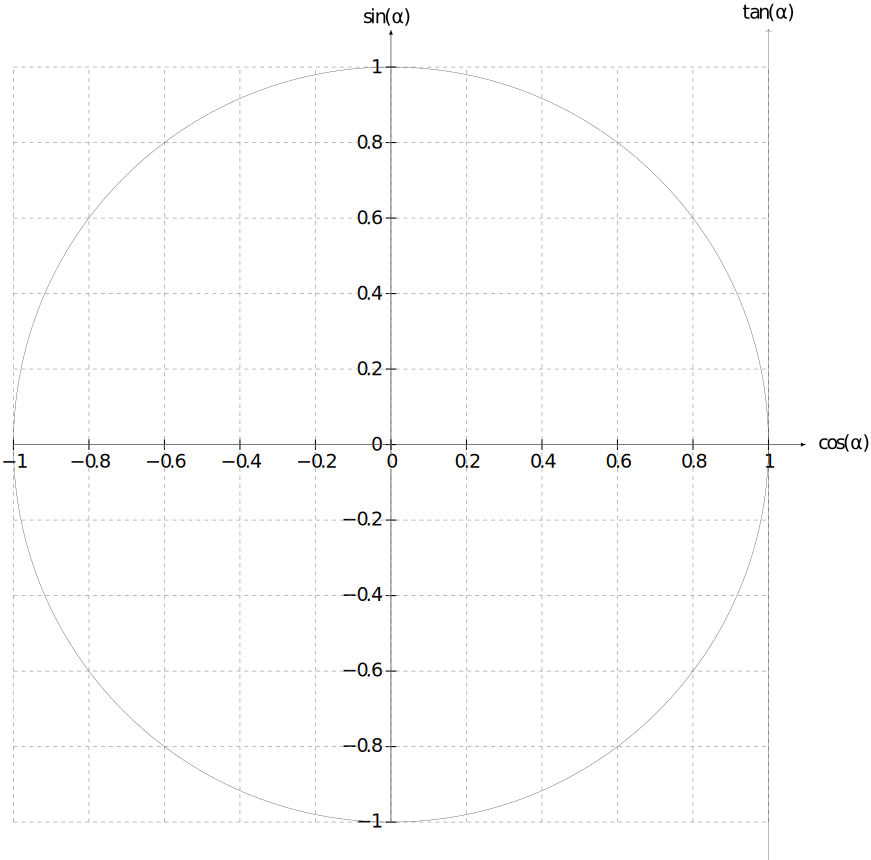
\includegraphics[width=0.4\textwidth,height=\textheight]{figures/CTT.pdf}
\end{center}

Ainsi, la tangente doit satisfaire une condition d'existence:
\(\tan(\alpha)\) existe à condition que \(\alpha\neq 90\) et
\(\alpha\neq 270\).

\end{tcolorbox}

La relation suivante donne un lien entre les différents nombres
trigonométriques.

\begin{theorem}[]\protect\hypertarget{thm-tan}{}\label{thm-tan}

Quel que soit \(\alpha\in[0;360]\), si \(\alpha\neq 90\) et
\(\alpha\neq 270\), alors

\[
\tan(\alpha)=\dfrac{\sin(\alpha)}{\cos(\alpha)}.
\]

\end{theorem}

\subsection{Représentation dans chaque
quadrant}\label{repruxe9sentation-dans-chaque-quadrant-1}

\begin{center}
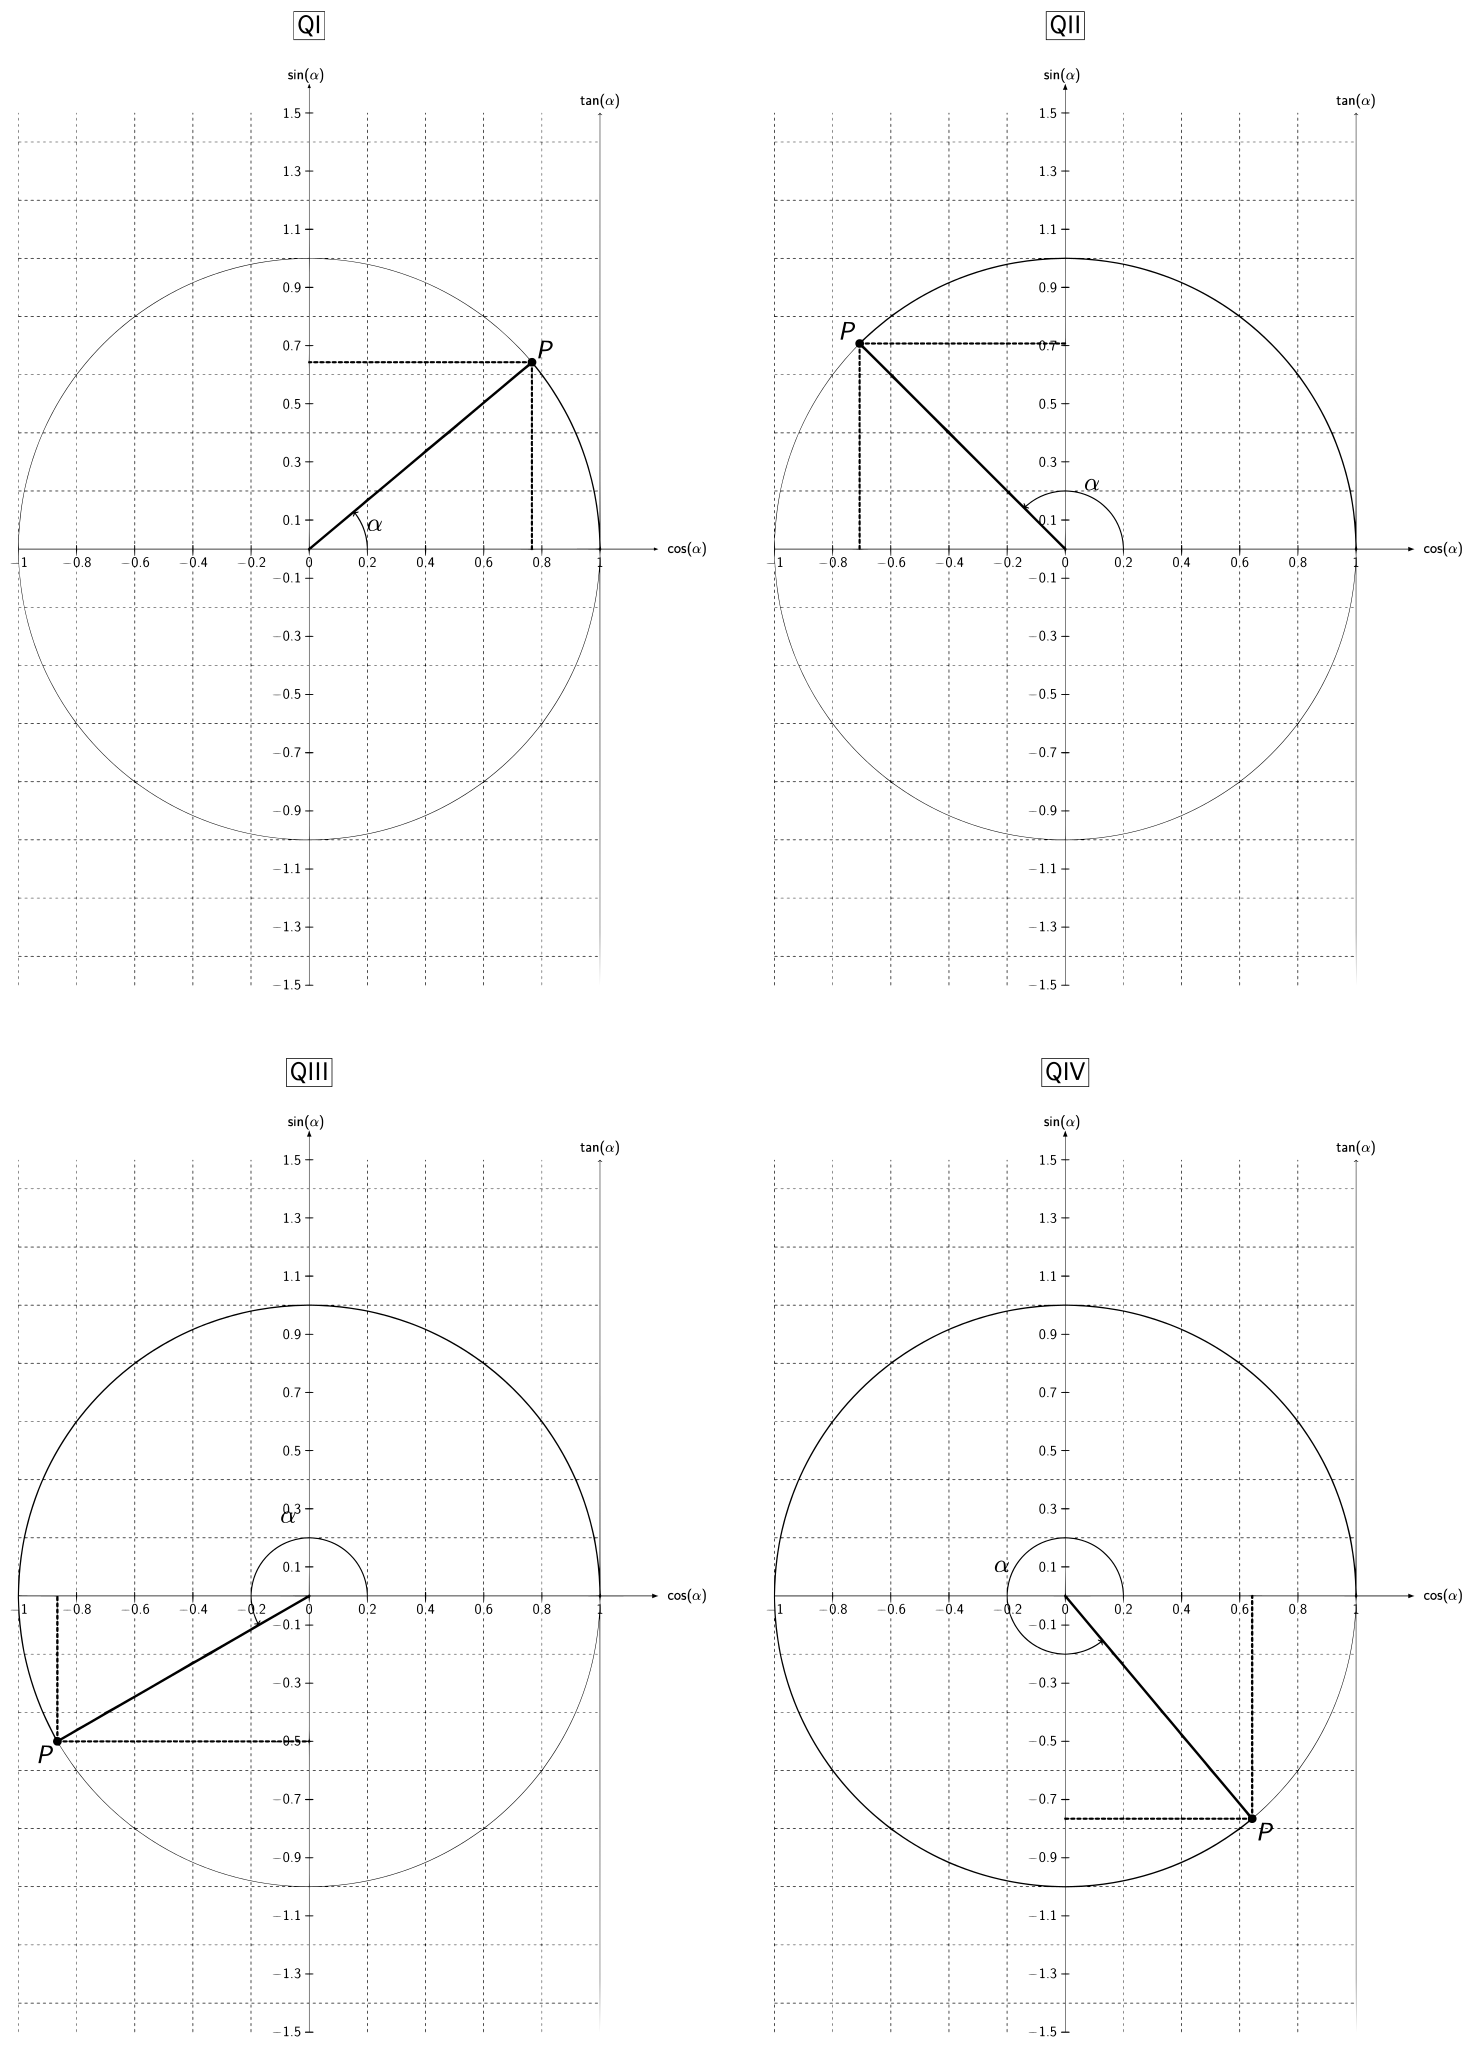
\includegraphics[width=0.65\textwidth,height=\textheight]{figures/fig34.pdf}
\end{center}

\begin{exercise}[]\protect\hypertarget{exr-signe-sincos}{}\label{exr-signe-sincos}

Complète les pointillés avec les symboles \(<\) et \(>\). \begin{center}
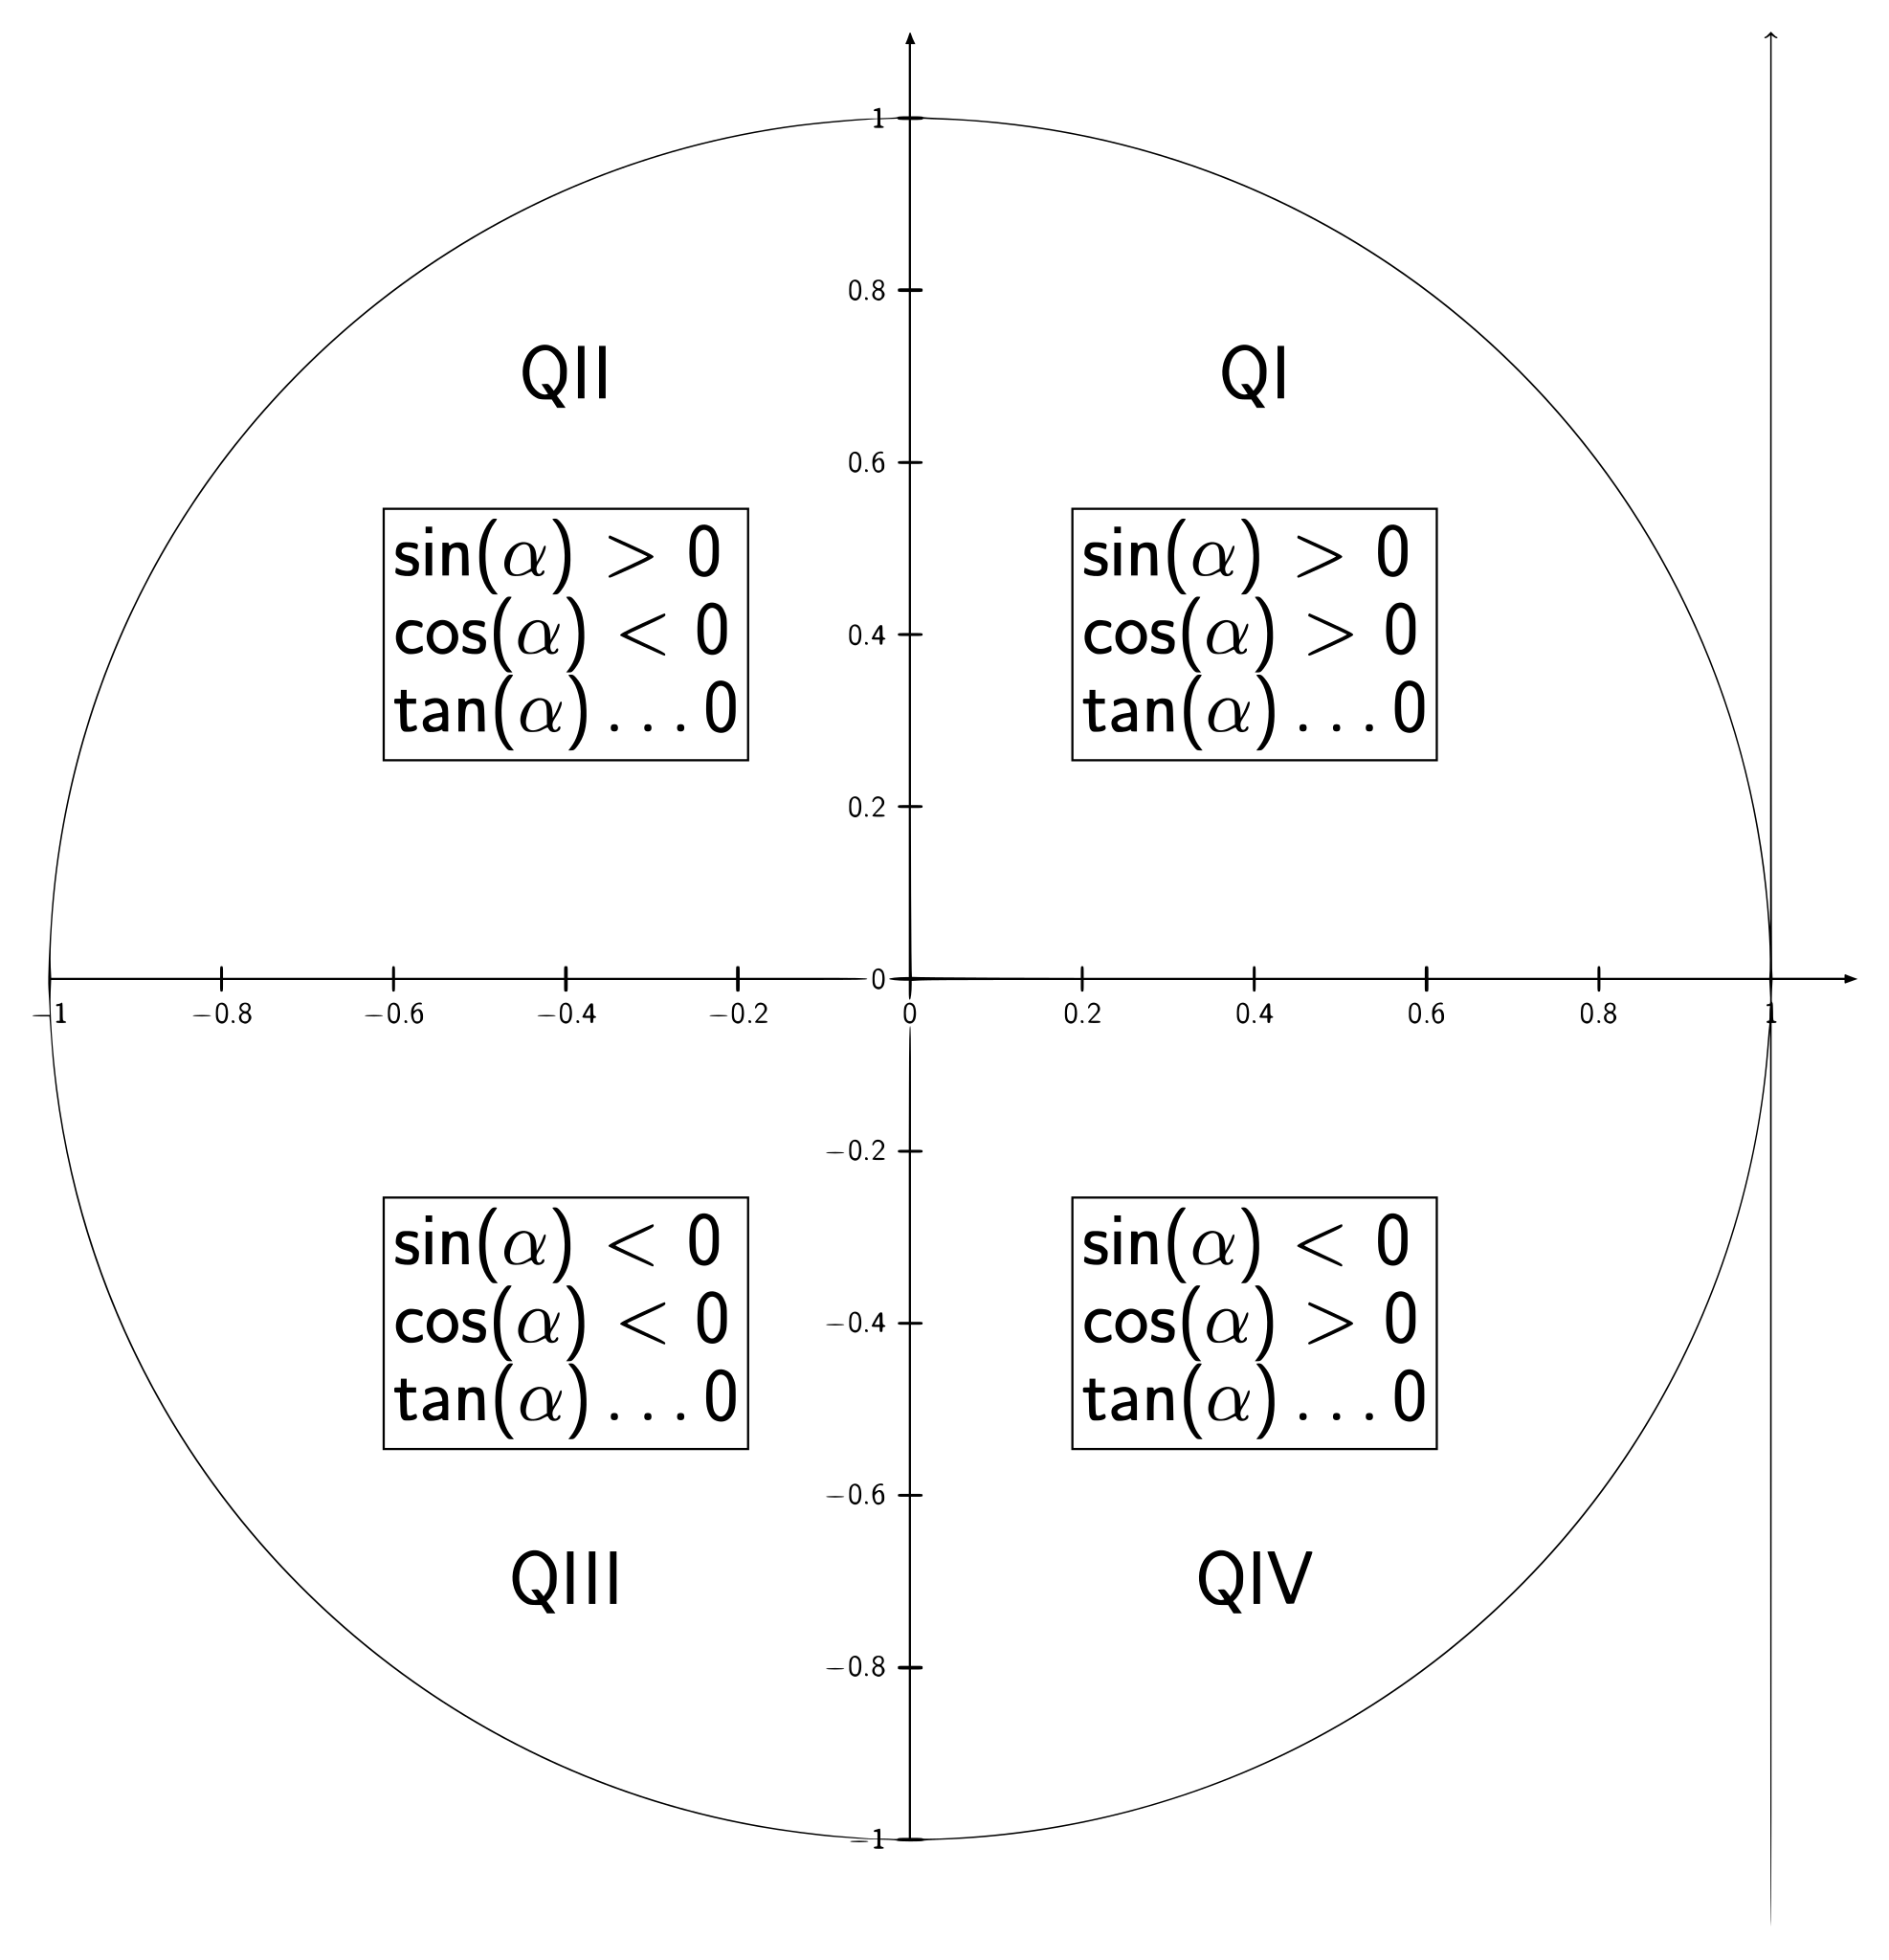
\includegraphics[width=0.4\textwidth,height=\textheight]{figures/fig33.pdf}
\end{center}

\end{exercise}

\subsection{Valeurs extrêmes et valeurs
particulières}\label{valeurs-extruxeames-et-valeurs-particuliuxe8res-1}

On a vu que le sinus et le consinus d'un angle est toujours compris
entre -1 et 1. Qu'en est-il pour la tangente?

\begin{exercise}[]\protect\hypertarget{exr-valtan}{}\label{exr-valtan}

A l'aide de la calculatrice, calcule les tangentes suivantes:

\begin{figure}

\begin{minipage}{0.33\linewidth}

\begin{enumerate}
\def\labelenumi{\arabic{enumi})}
\item
  \(\tan(89)=\) \dotfill
\item
  \(\tan(89,9)=\) \dotfill
\item
  \(\tan(89,99)=\) \dotfill
\item
  \(\tan(89,9999)=\) \dotfill
\item
  \(\tan(90)=\) \dotfill
\end{enumerate}

\end{minipage}%
%
\begin{minipage}{0.33\linewidth}

\begin{enumerate}
\def\labelenumi{\arabic{enumi})}
\setcounter{enumi}{5}
\item
  \(\tan(90,0001)=\) \dotfill
\item
  \(\tan(90,001)=\) \dotfill
\item
  \(\tan(90,01)=\) \dotfill
\item
  \(\tan(270,01)=\) \dotfill
\item
  \(\tan(270,001)=\) \dotfill
\end{enumerate}

\end{minipage}%
%
\begin{minipage}{0.34\linewidth}

\begin{enumerate}
\def\labelenumi{\arabic{enumi})}
\setcounter{enumi}{10}
\item
  \(\tan(270,0001)=\) \dotfill
\item
  \(\tan(269,9)=\) \dotfill
\item
  \(\tan(269,99)=\) \dotfill
\item
  \(\tan(269,999)=\) \dotfill
\item
  \(\tan(269,9999)=\) \dotfill
\end{enumerate}

\end{minipage}%

\end{figure}%

\end{exercise}

En conclusion, la \(\tan(\alpha)\) peut prendre \dotfill

Aux valeurs particulières des sinus et cosinus s'ajoutent les valeurs
particulières des tangentes. Elles doivent aussi être connues par coeur.

\begin{center}
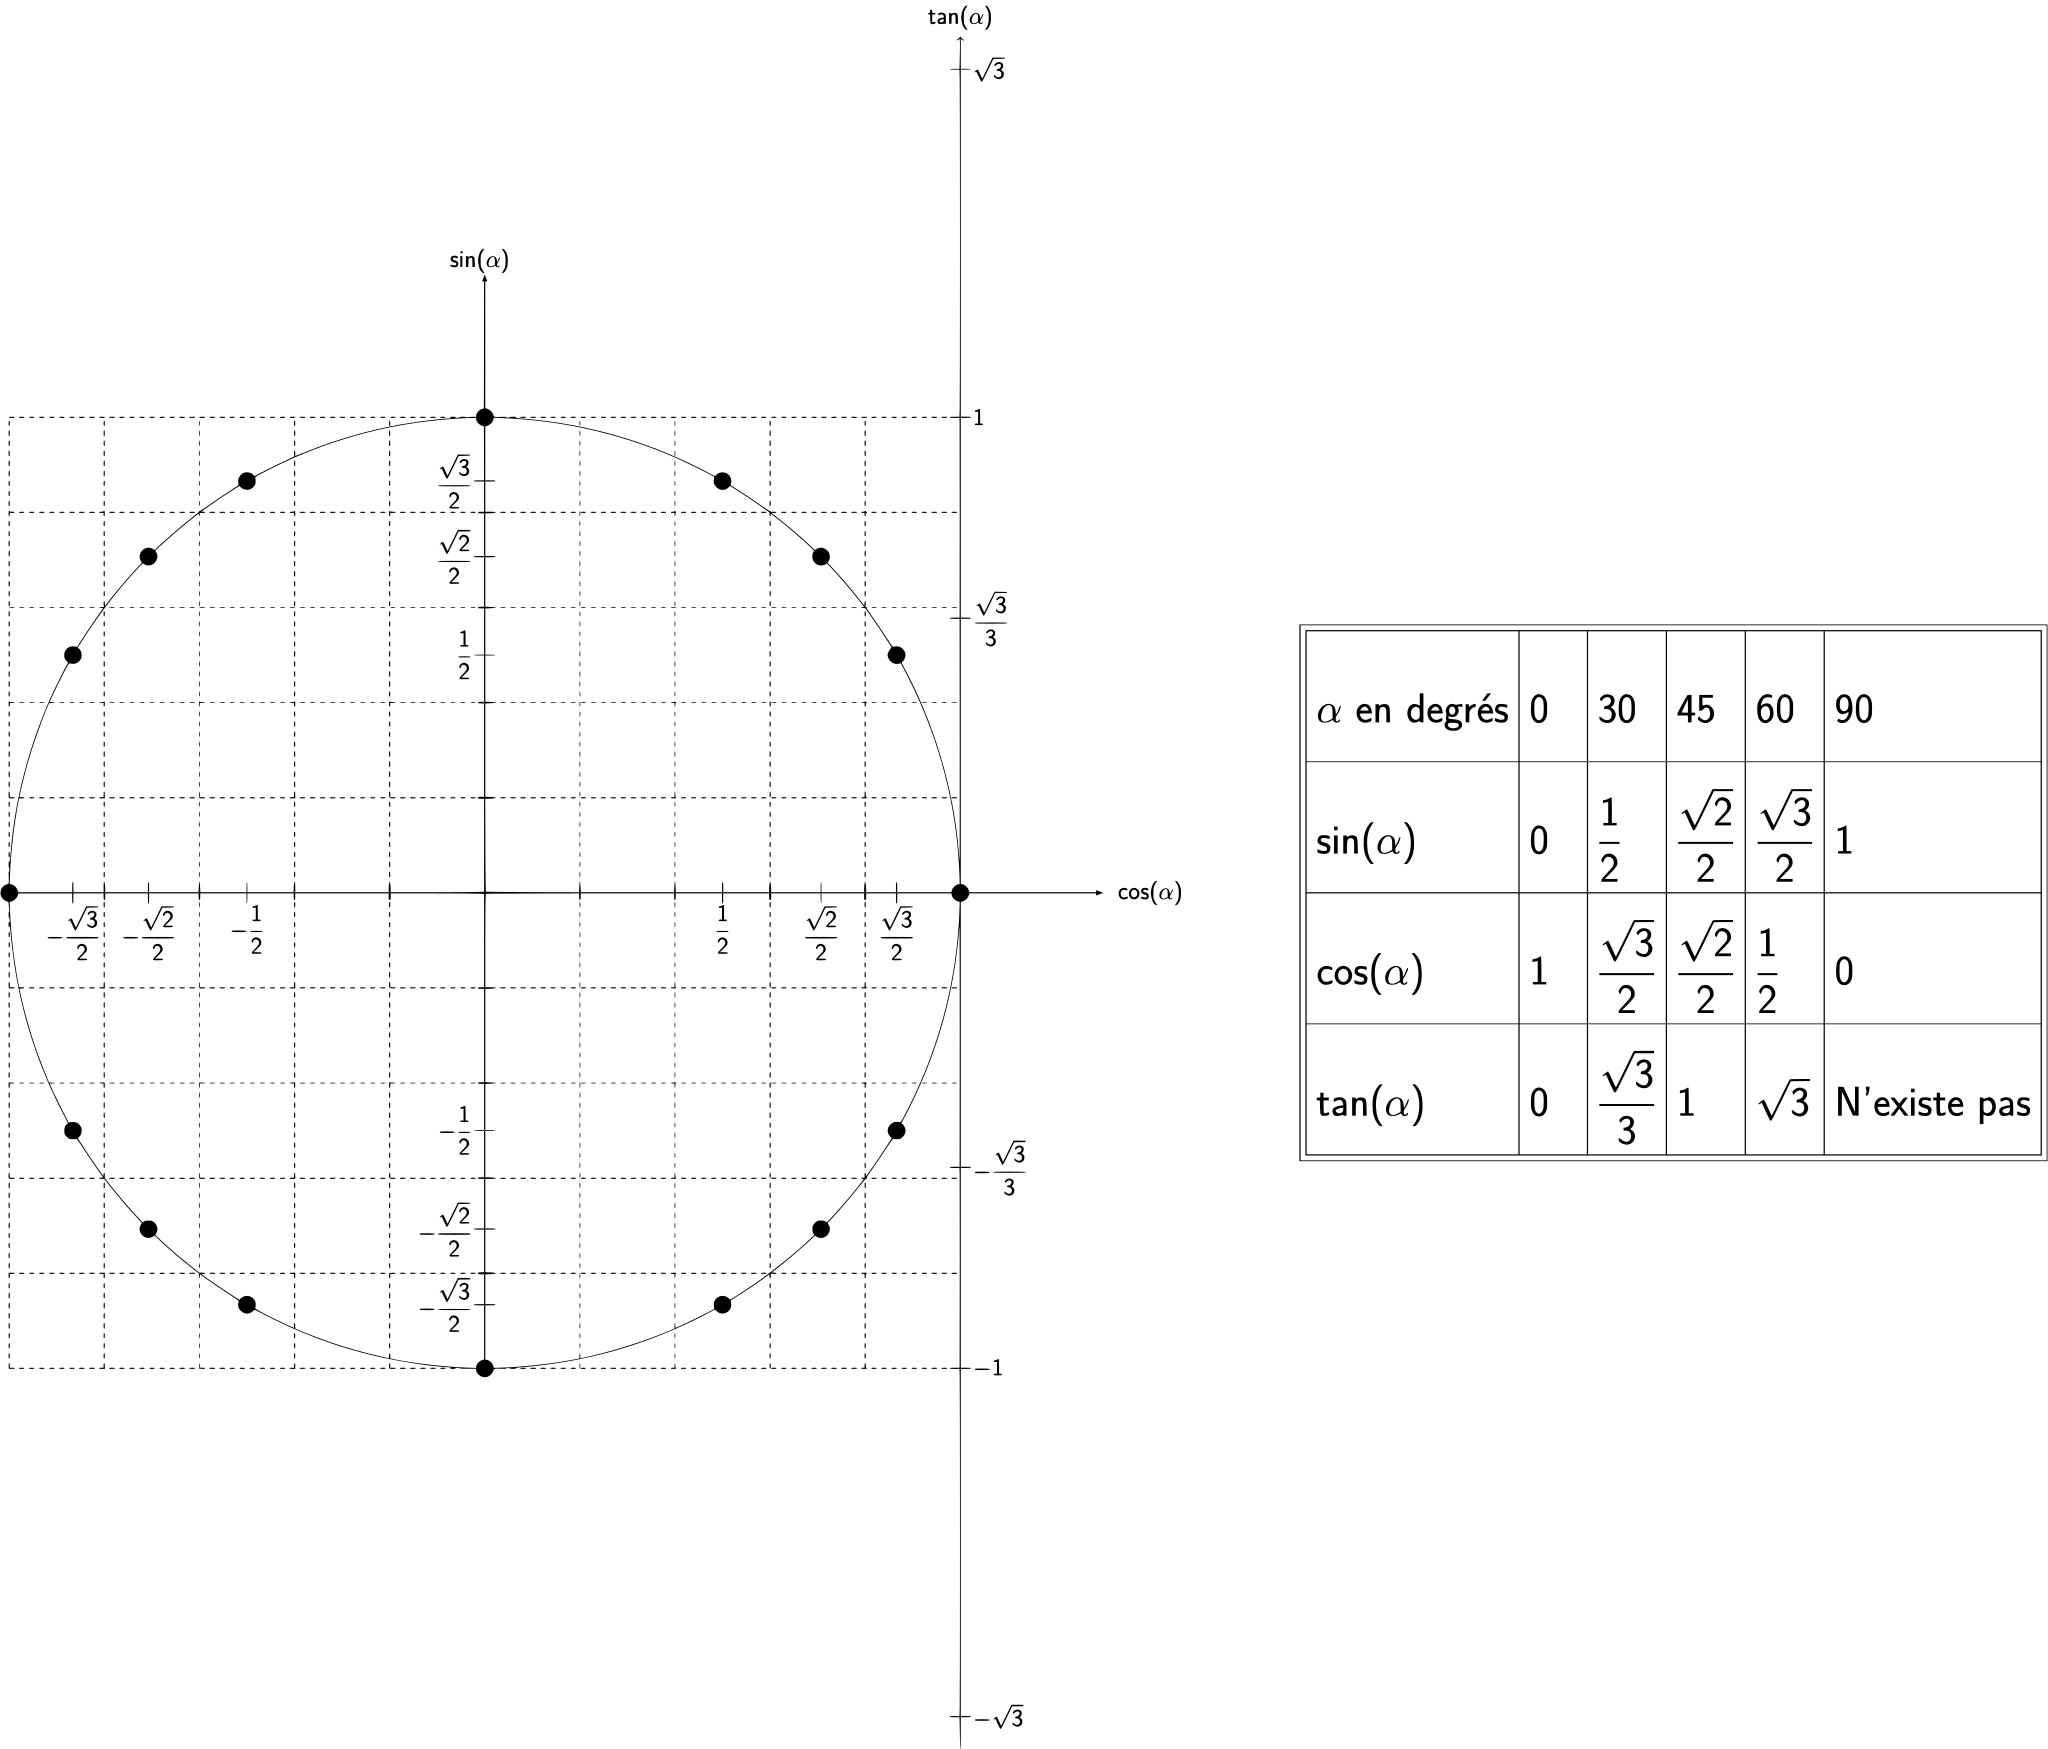
\includegraphics[width=1\textwidth,height=\textheight]{figures/fig35.pdf}
\end{center}

\subsection{Exercices}\label{exercices-2}

\begin{exercise}[]\protect\hypertarget{exr-}{}\label{exr-}

Représente sur le cercle trigonométrique les angles d'amplitude
\(25^\circ\), \(130^\circ\), \(225^\circ\) et \(330^\circ\) ainsi que
leur tangente.

\begin{center}
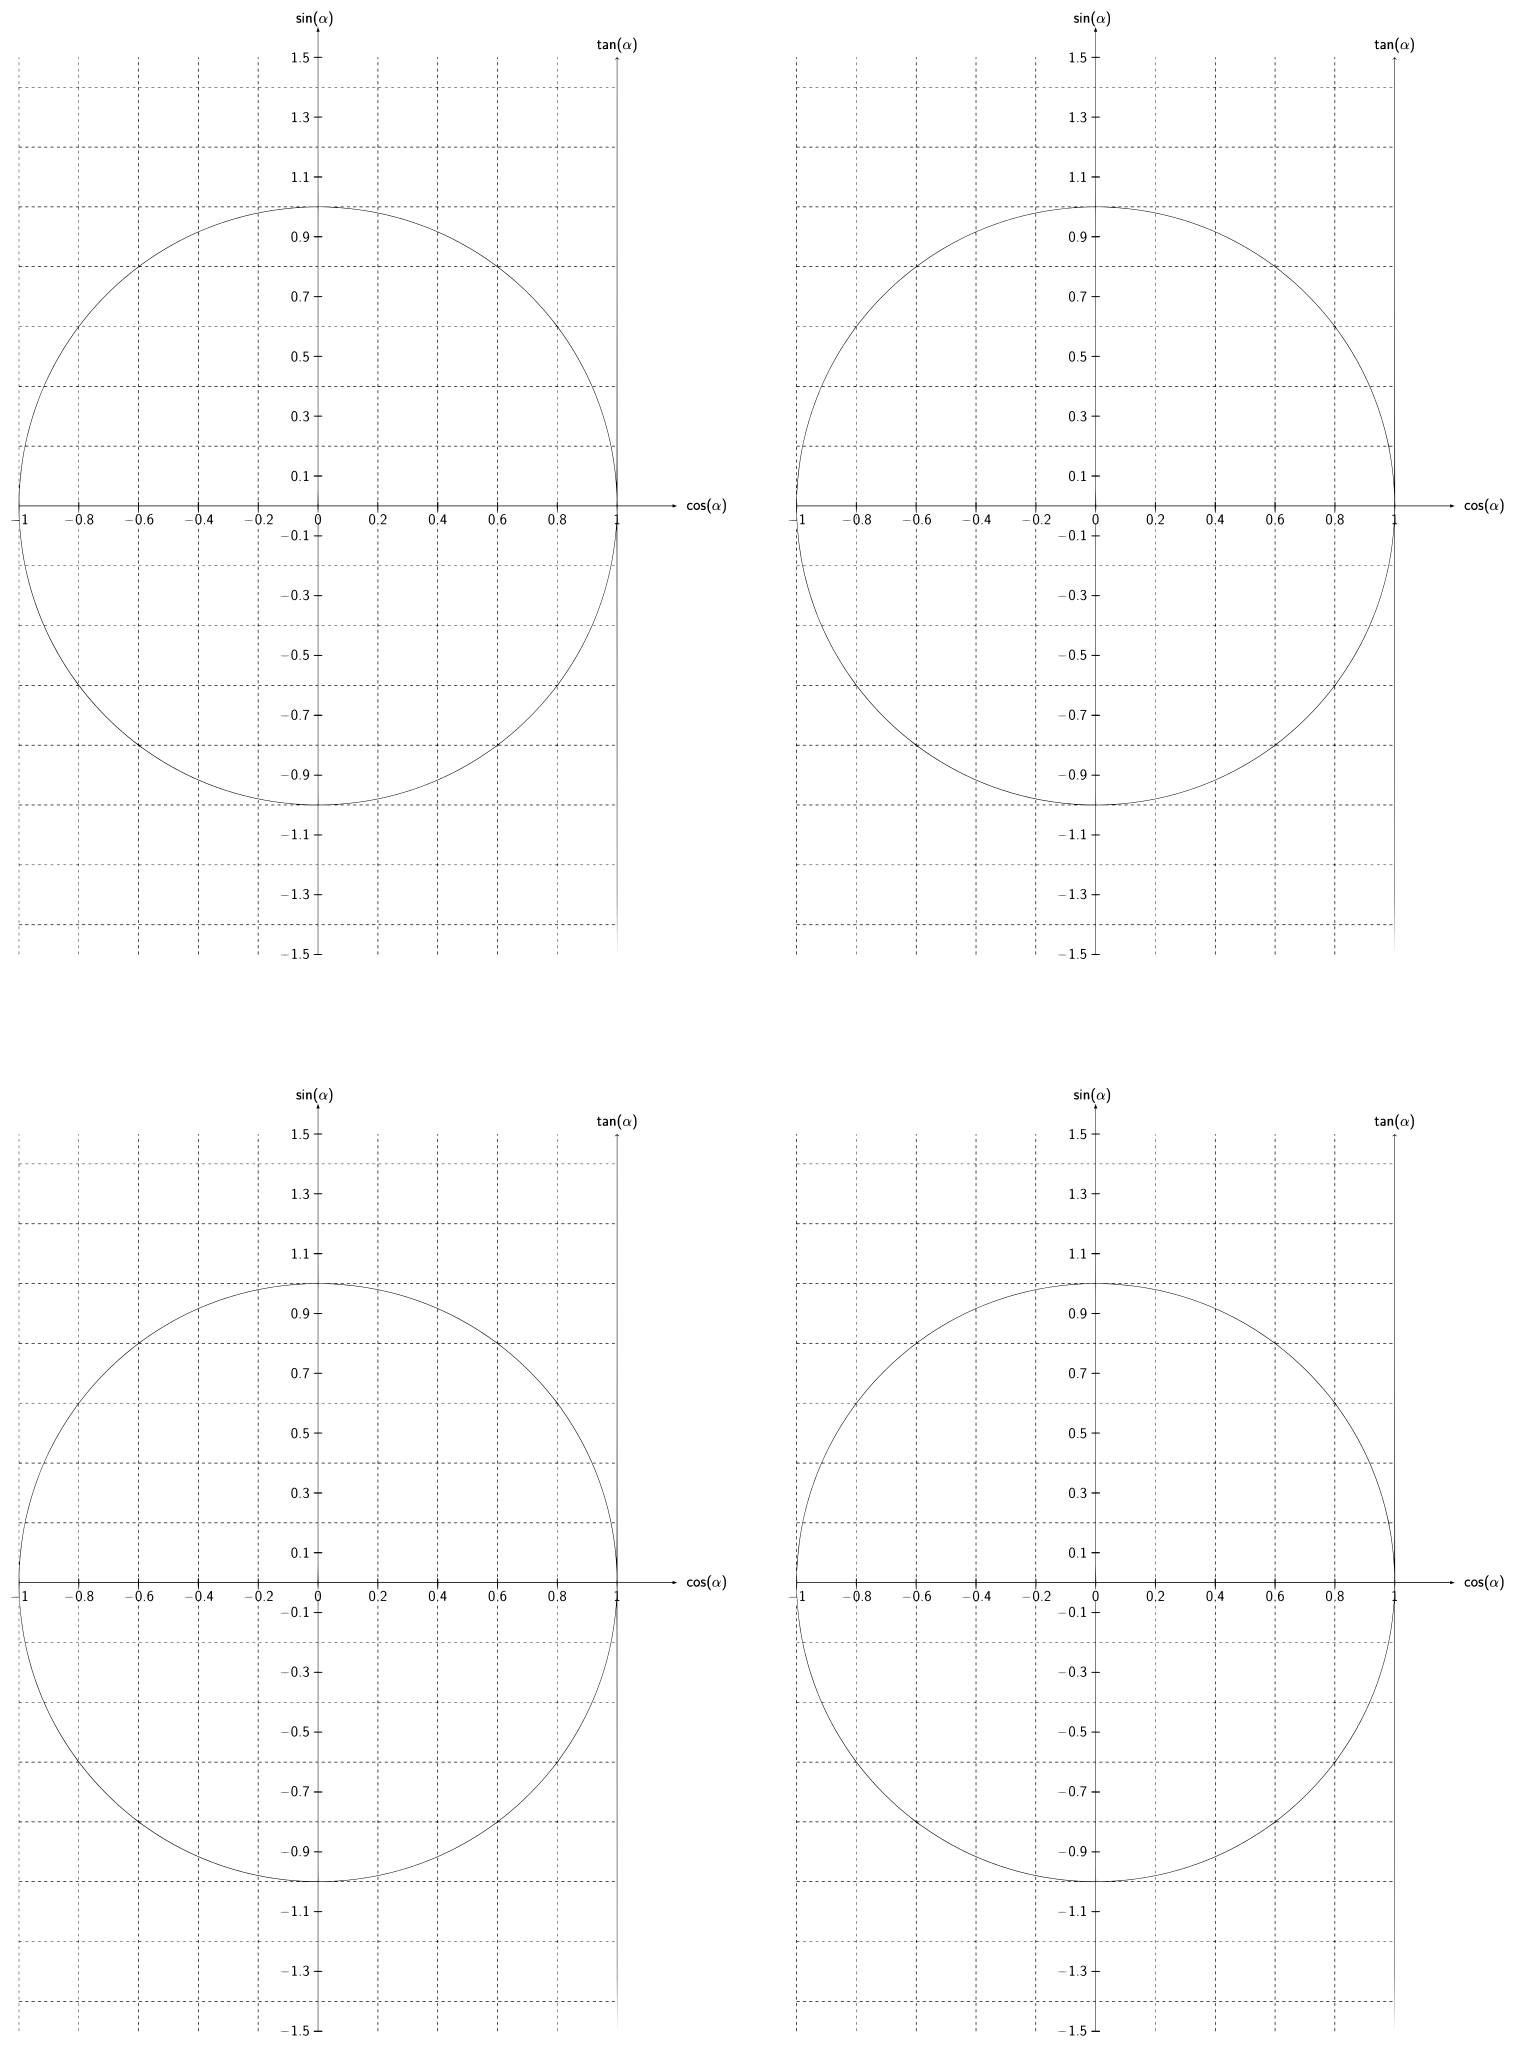
\includegraphics[width=1\textwidth,height=\textheight]{figures/fig31.pdf}
\end{center}

\end{exercise}

\begin{exercise}[]\protect\hypertarget{exr-}{}\label{exr-}

Complète par \(>\), \(<\) ou \(=\).

\begin{figure}

\begin{minipage}{0.60\linewidth}

\begin{enumerate}
\def\labelenumi{\arabic{enumi})}
\item
  \(\tan(-45)\makebox[2cm]{\dotfill}0\)
\item
  \(\tan(35)\makebox[2cm]{\dotfill}0\)
\item
  \(\tan(150)\makebox[2cm]{\dotfill}0\)
\end{enumerate}

\end{minipage}%
%
\begin{minipage}{0.40\linewidth}

\begin{enumerate}
\def\labelenumi{\arabic{enumi})}
\item
  \(\tan(250)\makebox[2cm]{\dotfill}0\)
\item
  \(\tan(180)\makebox[2cm]{\dotfill}0\)
\item
  \(\tan(-20)\makebox[2cm]{\dotfill}0\)
\end{enumerate}

\end{minipage}%

\end{figure}%

\end{exercise}

\begin{exercise}[]\protect\hypertarget{exr-}{}\label{exr-}

Sans passer par le calcul de l'angle, représente dans le cercle
trigonométrique les angles pour lesquels \(\tan(\alpha) = 0,9\).

\begin{center}
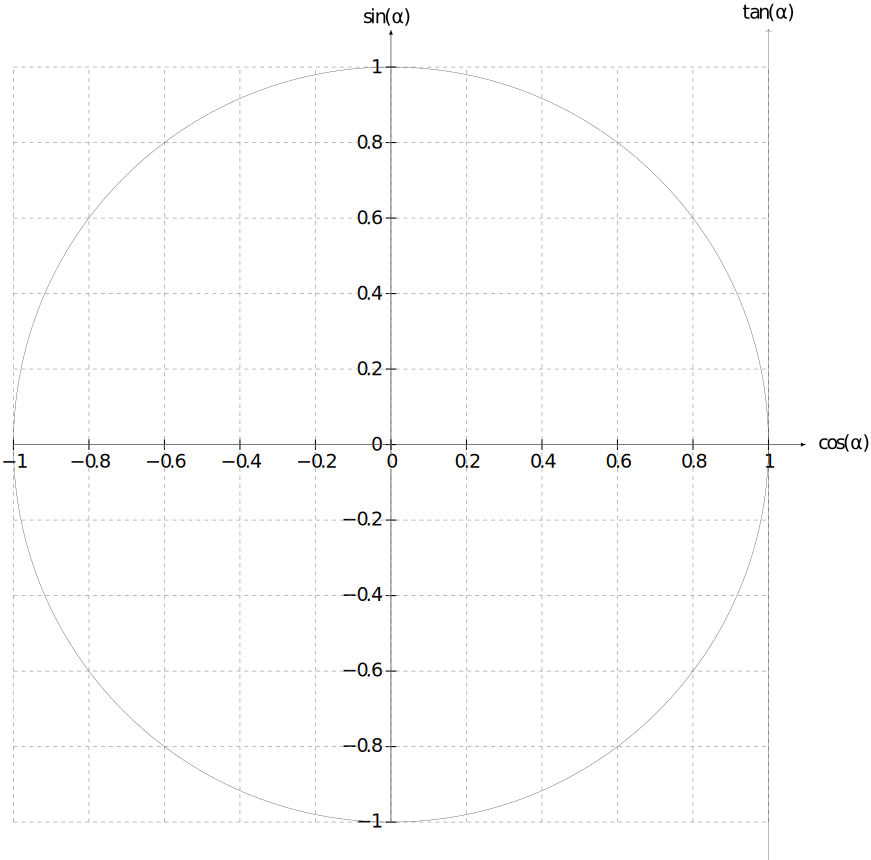
\includegraphics[width=0.5\textwidth,height=\textheight]{figures/CTT.pdf}
\end{center}

\end{exercise}

\begin{exercise}[]\protect\hypertarget{exr-}{}\label{exr-}

Sachant que \(\tan(40) \simeq 0,4\), détermine la valeur approximative
des tangentes suivantes.

\begin{figure}

\begin{minipage}{0.60\linewidth}

\begin{enumerate}
\def\labelenumi{\arabic{enumi})}
\item
  \(\tan(140)\simeq\makebox[2cm]{\dotfill}\)
\item
  \(\tan(220)\simeq\makebox[2cm]{\dotfill}\)
\item
  \(\tan(320)\simeq\makebox[2cm]{\dotfill}\)
\end{enumerate}

\end{minipage}%
%
\begin{minipage}{0.40\linewidth}
\begin{center}
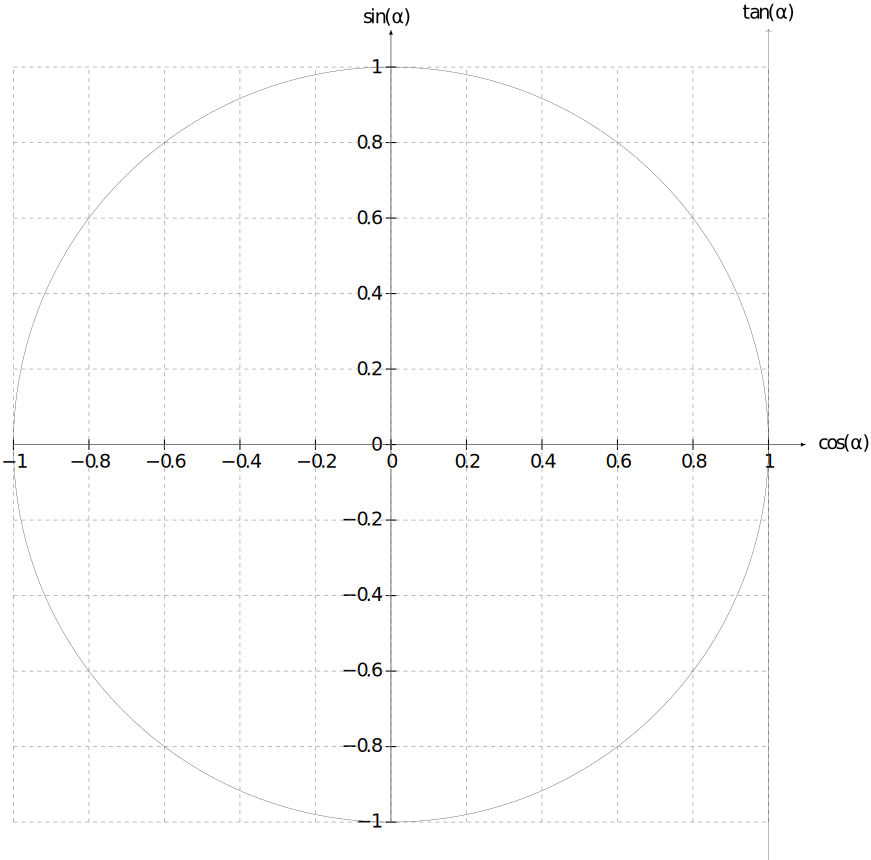
\includegraphics{figures/CTT.pdf}
\end{center}
\end{minipage}%

\end{figure}%

\end{exercise}

\begin{exercise}[]\protect\hypertarget{exr-}{}\label{exr-}

A l'aide de la calculatrice, détermine l'amplitude des angles (entre 0°
et 360°) dont la tangente vaut 0,5. Arrondis au dixième près si
nécessaire.

\end{exercise}

\begin{exercise}[]\protect\hypertarget{exr-}{}\label{exr-}

Sachant que \(\alpha\in\text{QIII}\) et que
\(\sin(\alpha) = \dfrac{-4}{5}\), calcule la valeur exacte de
\(\cos(\alpha)\) en utilisant la formule fondamentale de trigonométrie.
Calcule ensuite \(\tan(\alpha)\).

\end{exercise}




\end{document}
